\documentclass[22pt]{book}

\usepackage{graphicx}  % Required for inserting images
\usepackage{biblatex}  % Imports biblatex package
\usepackage{float}     % put images here
\addbibresource{bibliography.bib} % Import the bibliography file
% \usepackage{ragged2e}  % justify text
\usepackage{amsmath,amssymb}  % math stuff
\usepackage[margin=0.75in]{geometry}  % margin
\raggedbottom

\title{PhD thesis}
\author{Maarten van der Sande}
\date{May 2023}

\makeatletter
\newcommand{\chapterauthor}[1]{%
  {\parindent0pt\vspace*{-25pt}%
  \linespread{1.1}\large\scshape#1%
  \par\nobreak\vspace*{35pt}}
  \@afterheading%
}
\makeatother
\newcommand{\beginsupplement}{
    \setcounter{table}{0}
    \renewcommand{\thetable}{S\thechapter.\arabic{table}}%
    \setcounter{figure}{0}
    \renewcommand{\thefigure}{S\thechapter.\arabic{figure}}%
}
\newcommand{\closesupplement}{
    \renewcommand{\thetable}{\thechapter.\arabic{table}}
    \renewcommand{\thefigure}{\thechapter.\arabic{figure}}
}

% table of content
% \setcounter{tocdepth}{1}


\begin{document}

\maketitle

\tableofcontents

\chapter{General introduction}
\section{The central dogma of molecular biology}

The human body is formed by a collection of 37,000,000,000,000 cells\cite{Bianconi2013}, with each cell containing approximately 2 meters of DNA. This means that our bodies house an astounding 74,000,000,000 kilometers of DNA, which is equivalent to almost 250 round trips to the sun! Our DNA is organized into 20,000 genes, spread across 23 distinct structures called chromosomes. What makes all this even more intriguing is that all cells within our body possess exactly the same DNA, yet they exhibit remarkable diversity and specialization. How does this single set of instructions give rise to such diverse cell types? What is the role of DNA during (embryonic) development? And how does this process compare across different species? To better appreciate these fascinating phenomena, it is crucial to understand the central dogma of molecular biology (fig. \ref{fig:central_dogma}).

\begin{figure}[H]
    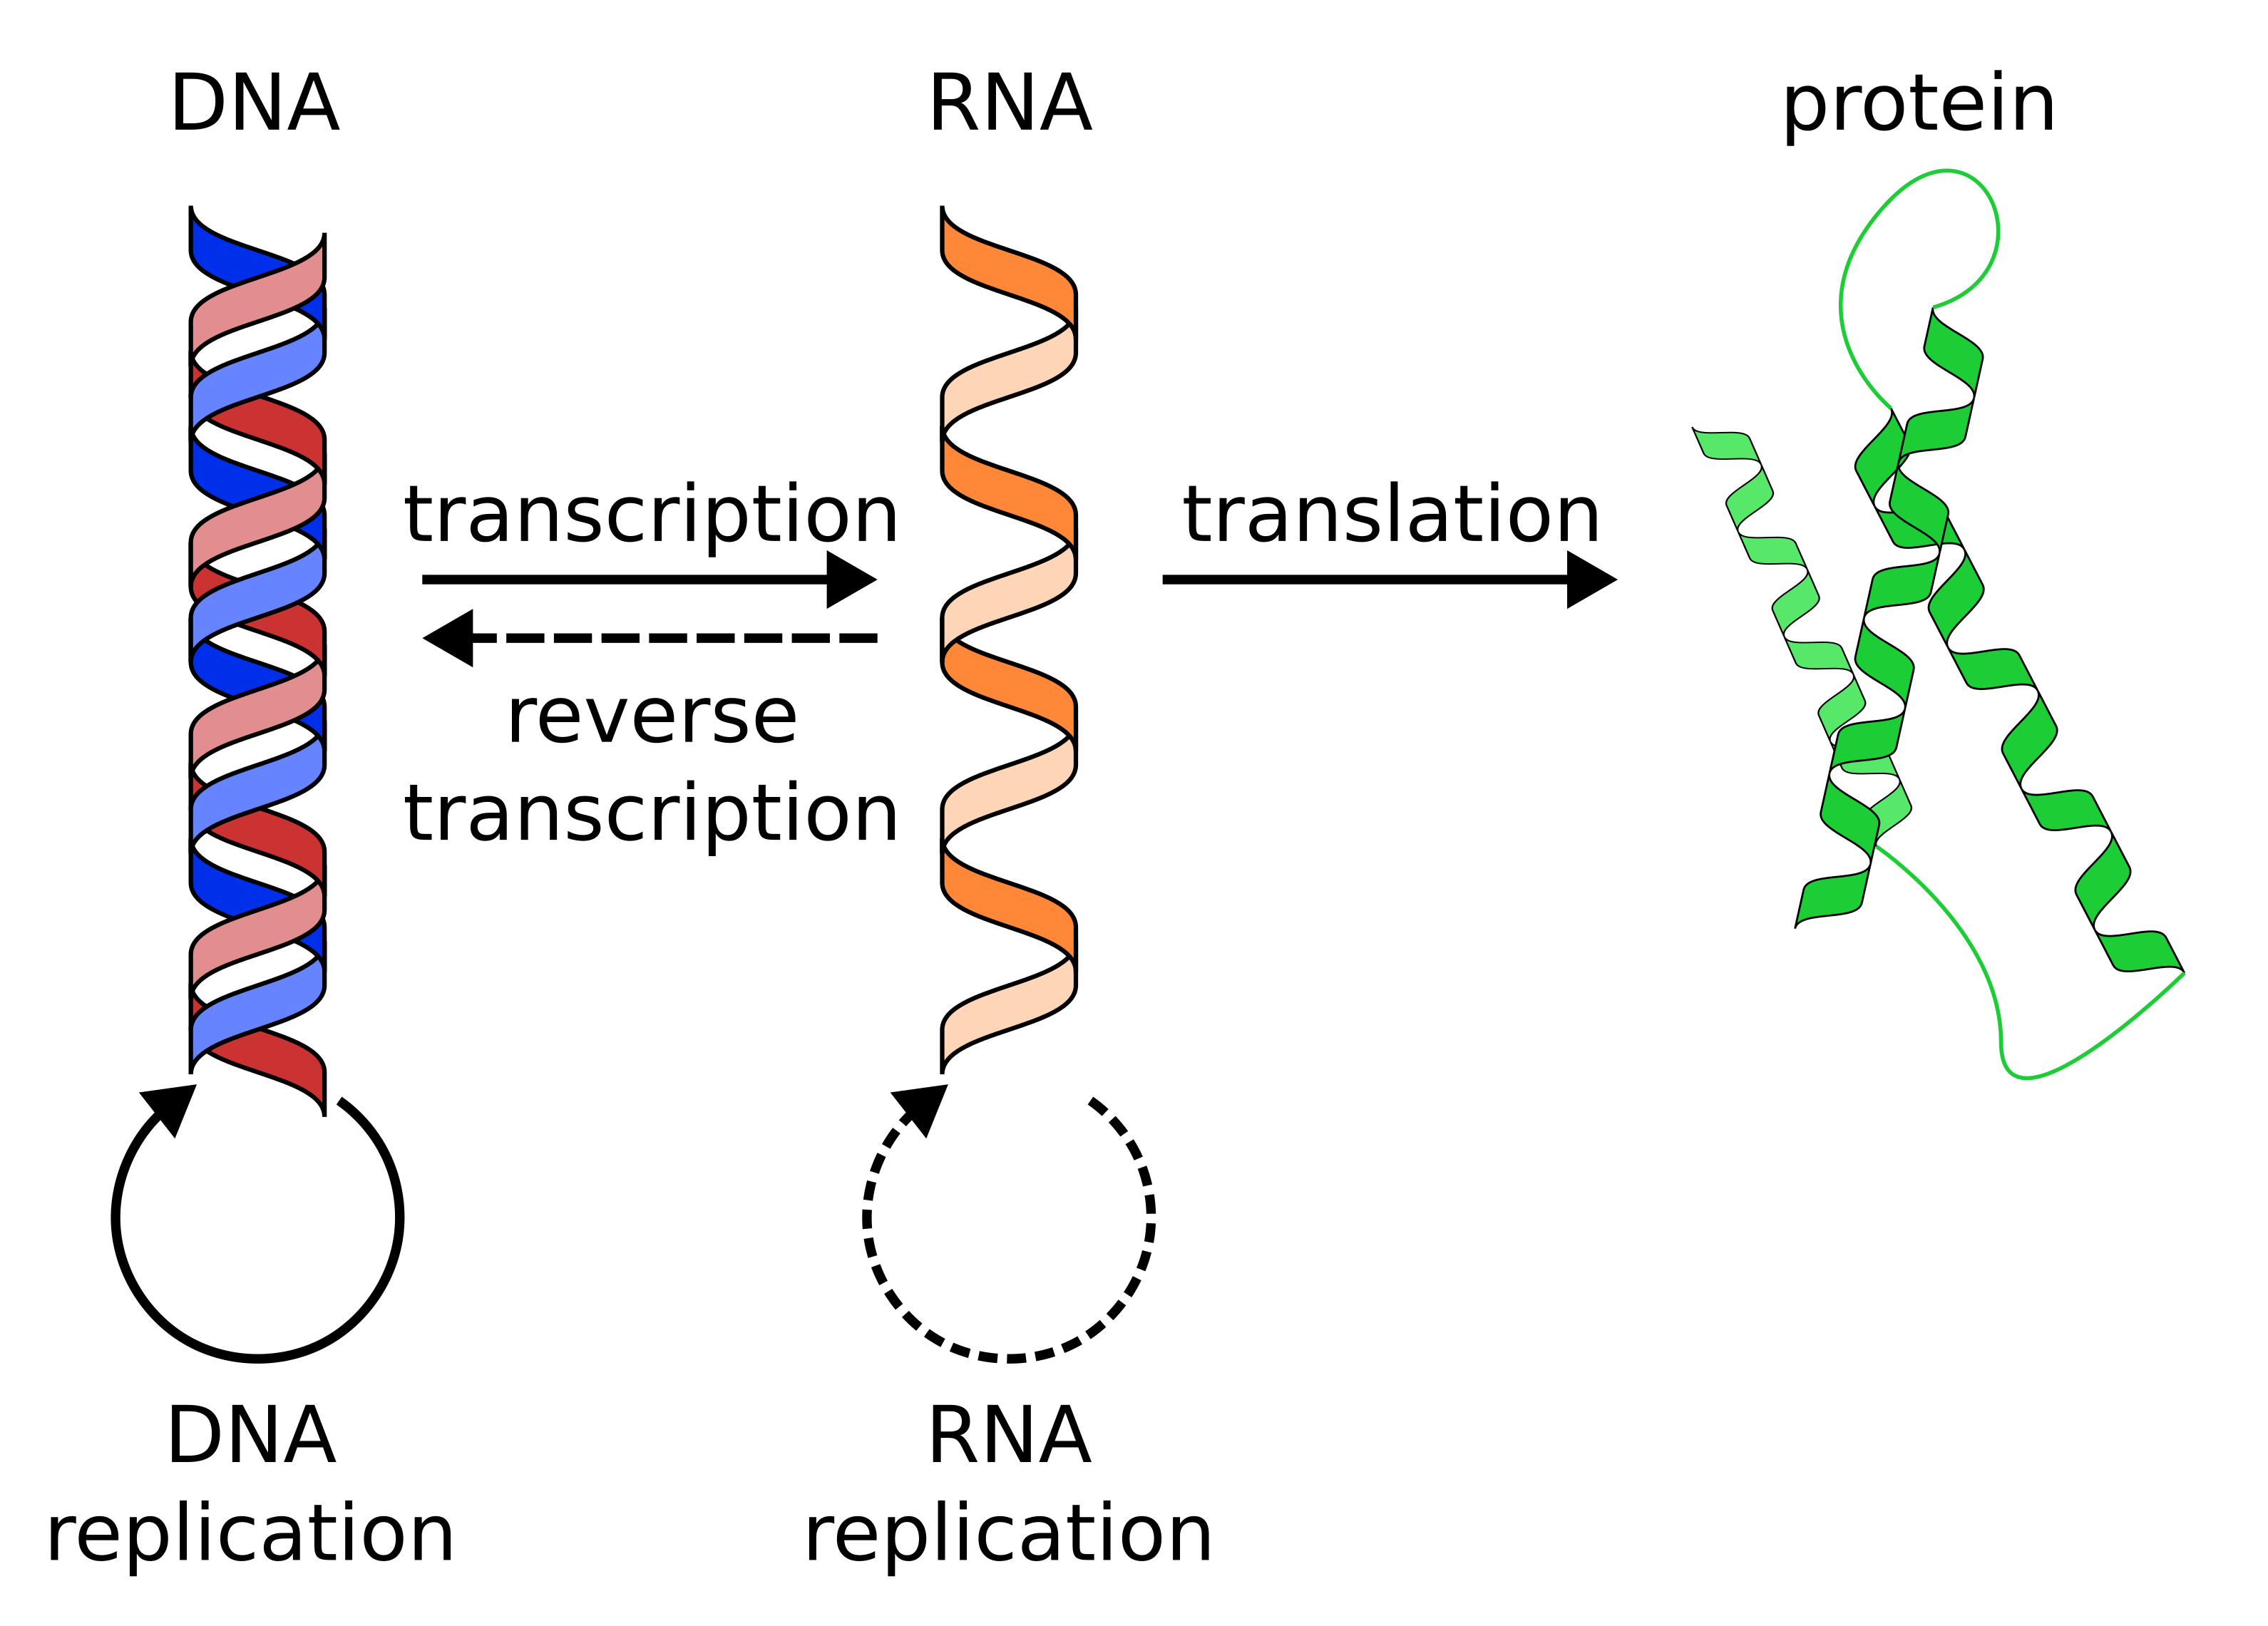
\includegraphics[width=\linewidth]{ch1.Introduction/imgs/central_dogma.png}
    \caption{The central dogma of molecular biology. Solid arrows indicate the general flow of information in the system, and dotted arrows special cases. }
    \label{fig:central_dogma}
\end{figure}

The central dogma of molecular biology describes the flow of genetic information within a biological system. Whereas in a computer information is stored in bits, which can be either zero (0) or one (1), genetic information is stored in nucleotides, which can be either adenine (A), cytosine (C), guanine (G), or thymine (T). DNA, which stands for deoxyribonucleic acid, is composed of two large strands of these nucleotides that together form a double helix. Both strands contain the same information, but where there is a nucleotide A on one strand, there is always a corresponding nucleotide T on the other, and similarly for C and G. RNA, on the other hand, is a similar molecule but is typically single-stranded. It is transcribed from DNA and shares a similar nucleotide composition but replaces thymine (T) with uracil (U). RNA serves as the bridge between DNA and proteins. Through the process of translation, the information encoded in RNA is decoded and used to assemble chains of amino acids, ultimately resulting in the synthesis of proteins. Proteins carry out various tasks in our bodies, such as enabling chemical reactions, transporting other molecules, providing structure, and acting as regulators of transcription and translation of genes.

Far from all the DNA is transcribed into RNA, and not even all RNA translates to protein. As a general rule of thumb, we distinguish DNA sequences that get transcribed into RNA as genes. The human genome consists of approximately 20.000 genes, and the coding parts of these genes represent approximately 6\% of the genome\cite{Piovesan2019}. Early molecular biologists mainly focused on coding genes, thus the remaining 94\% got known as ``junk DNA''. We now know, however, that at least 80\% of human DNA is involved in at least one biochemical function\cite{encode2012}. Almost all of these functions are related to gene expression regulation.

% \subsection{Transcription}

% \begin{figure}[hbtp]
%     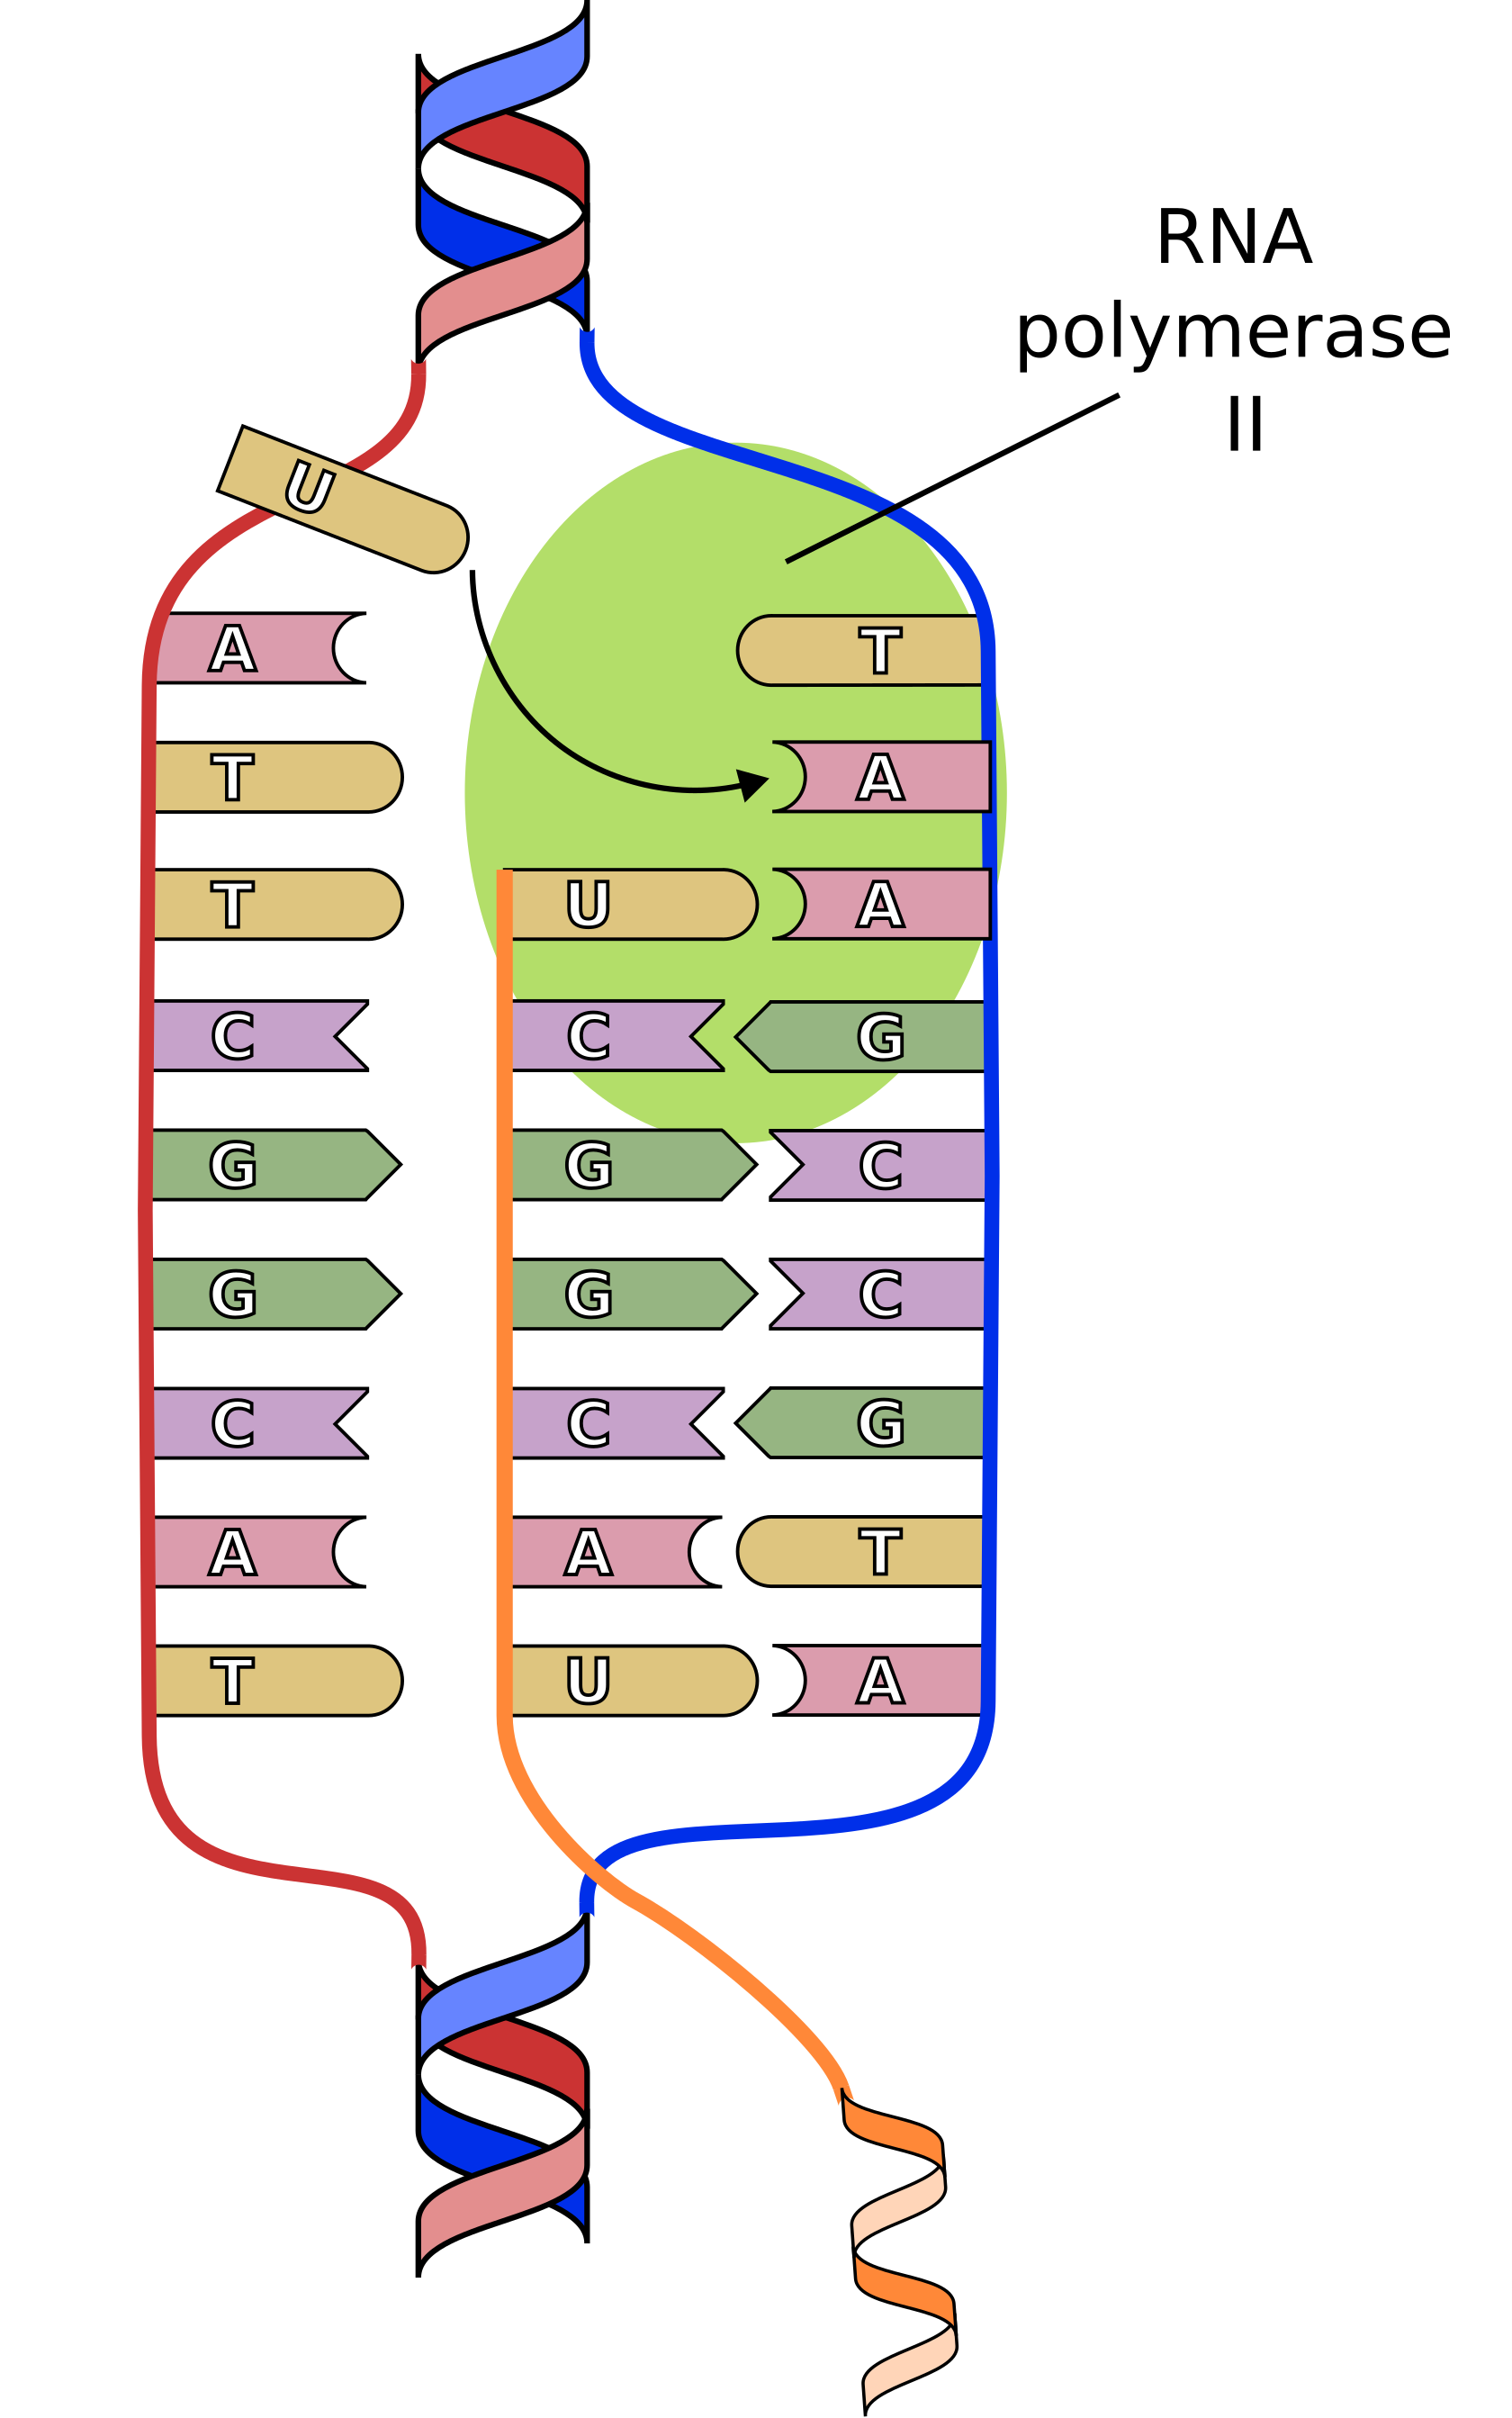
\includegraphics[height=0.5\textheight]{ch1.Introduction/imgs/transcription.png}
%     \caption{Caption}
%     \label{fig:transcription}
% \end{figure}

% \subsection{Translation}

% \begin{figure}[H]
%     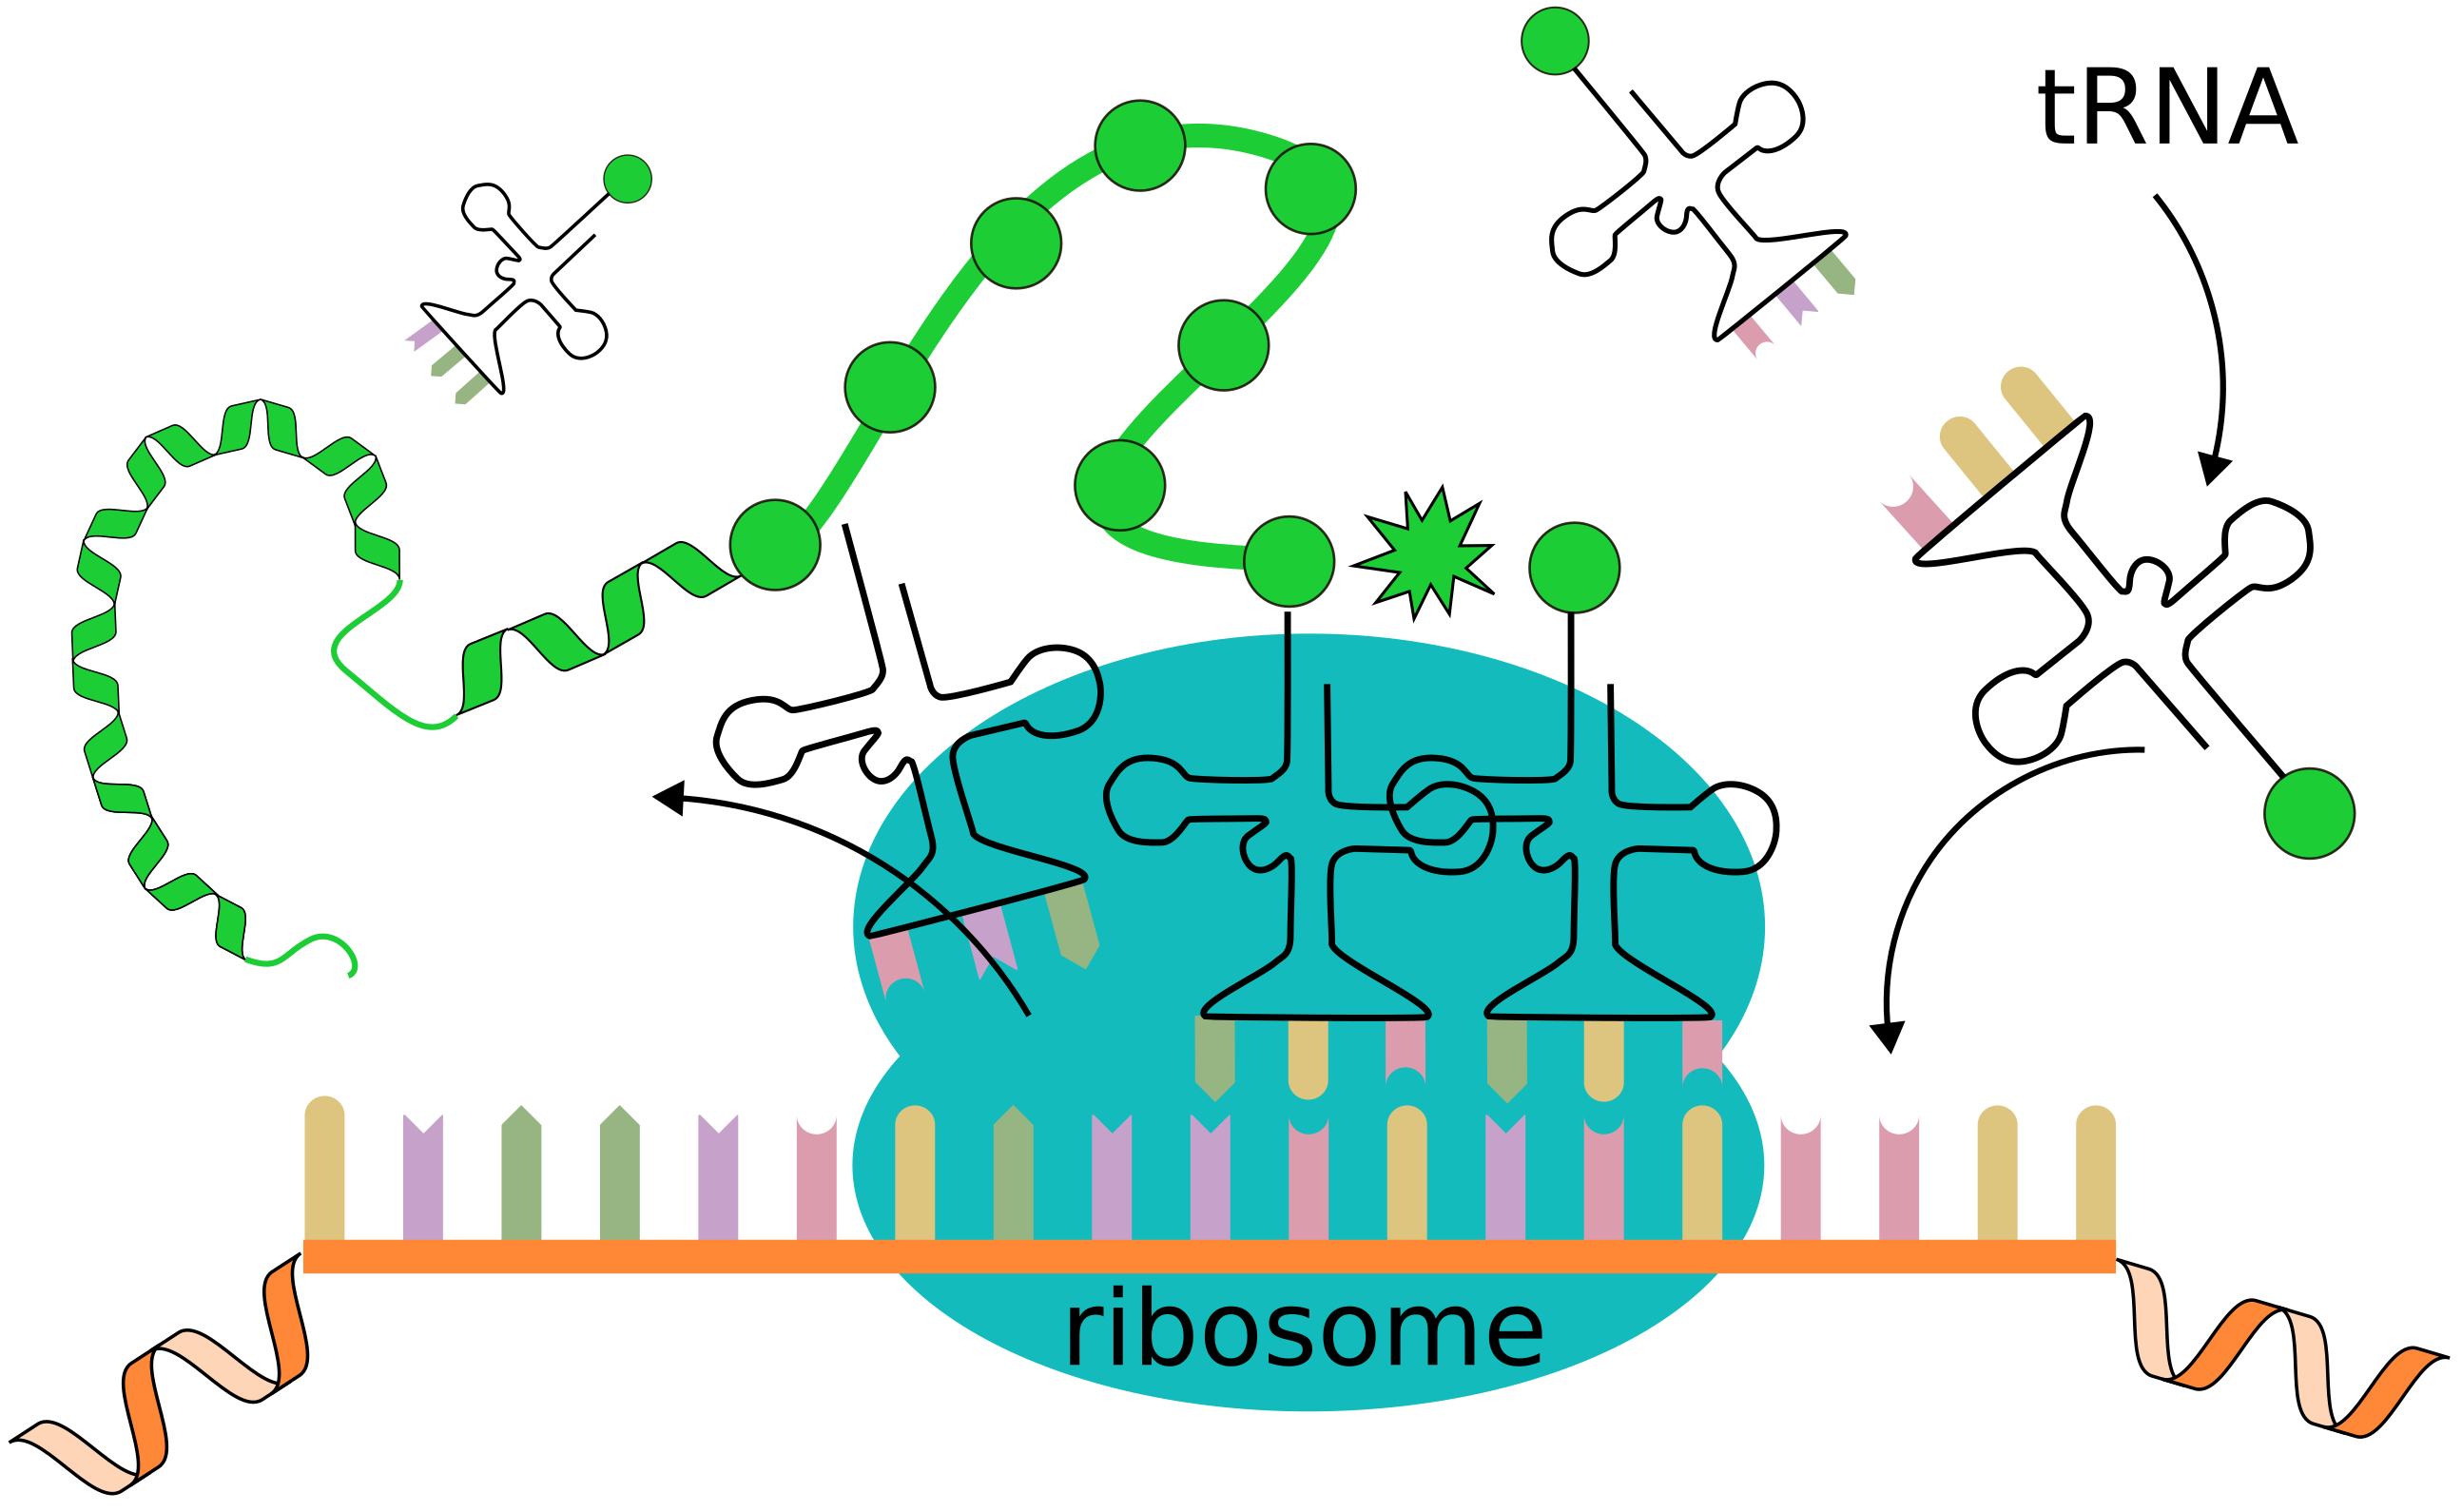
\includegraphics[width=\linewidth]{ch1.Introduction/imgs/translation.png}
%     \caption{Caption}
%     \label{fig:translation}
% \end{figure}

\section{Gene expression regulation}

A skin cell makes use of a completely different set of genes than a liver cell, even though they contain the same DNA. This is possible due to the tight regulation of gene expression by these cells. To regulate their gene expression cells have a wide array of tools at their disposal. 

\subsection{Transcription Factors}

At the start of each gene sits a promoter (fig. \ref{fig:TF}A). At the promoter general transcription factors bind, which in turn recruit RNA polymerase II (RNAPII). RNAPII is the protein complex responsible for transription, and in turn 

Before DNA transcription can occur, 

DNA transcription requires a wide array of steps. Slightly upstream of a gene is a promoter. To this piece of DNA proteins bind that initiate transcription.

motifs needed

\begin{figure}[H]
    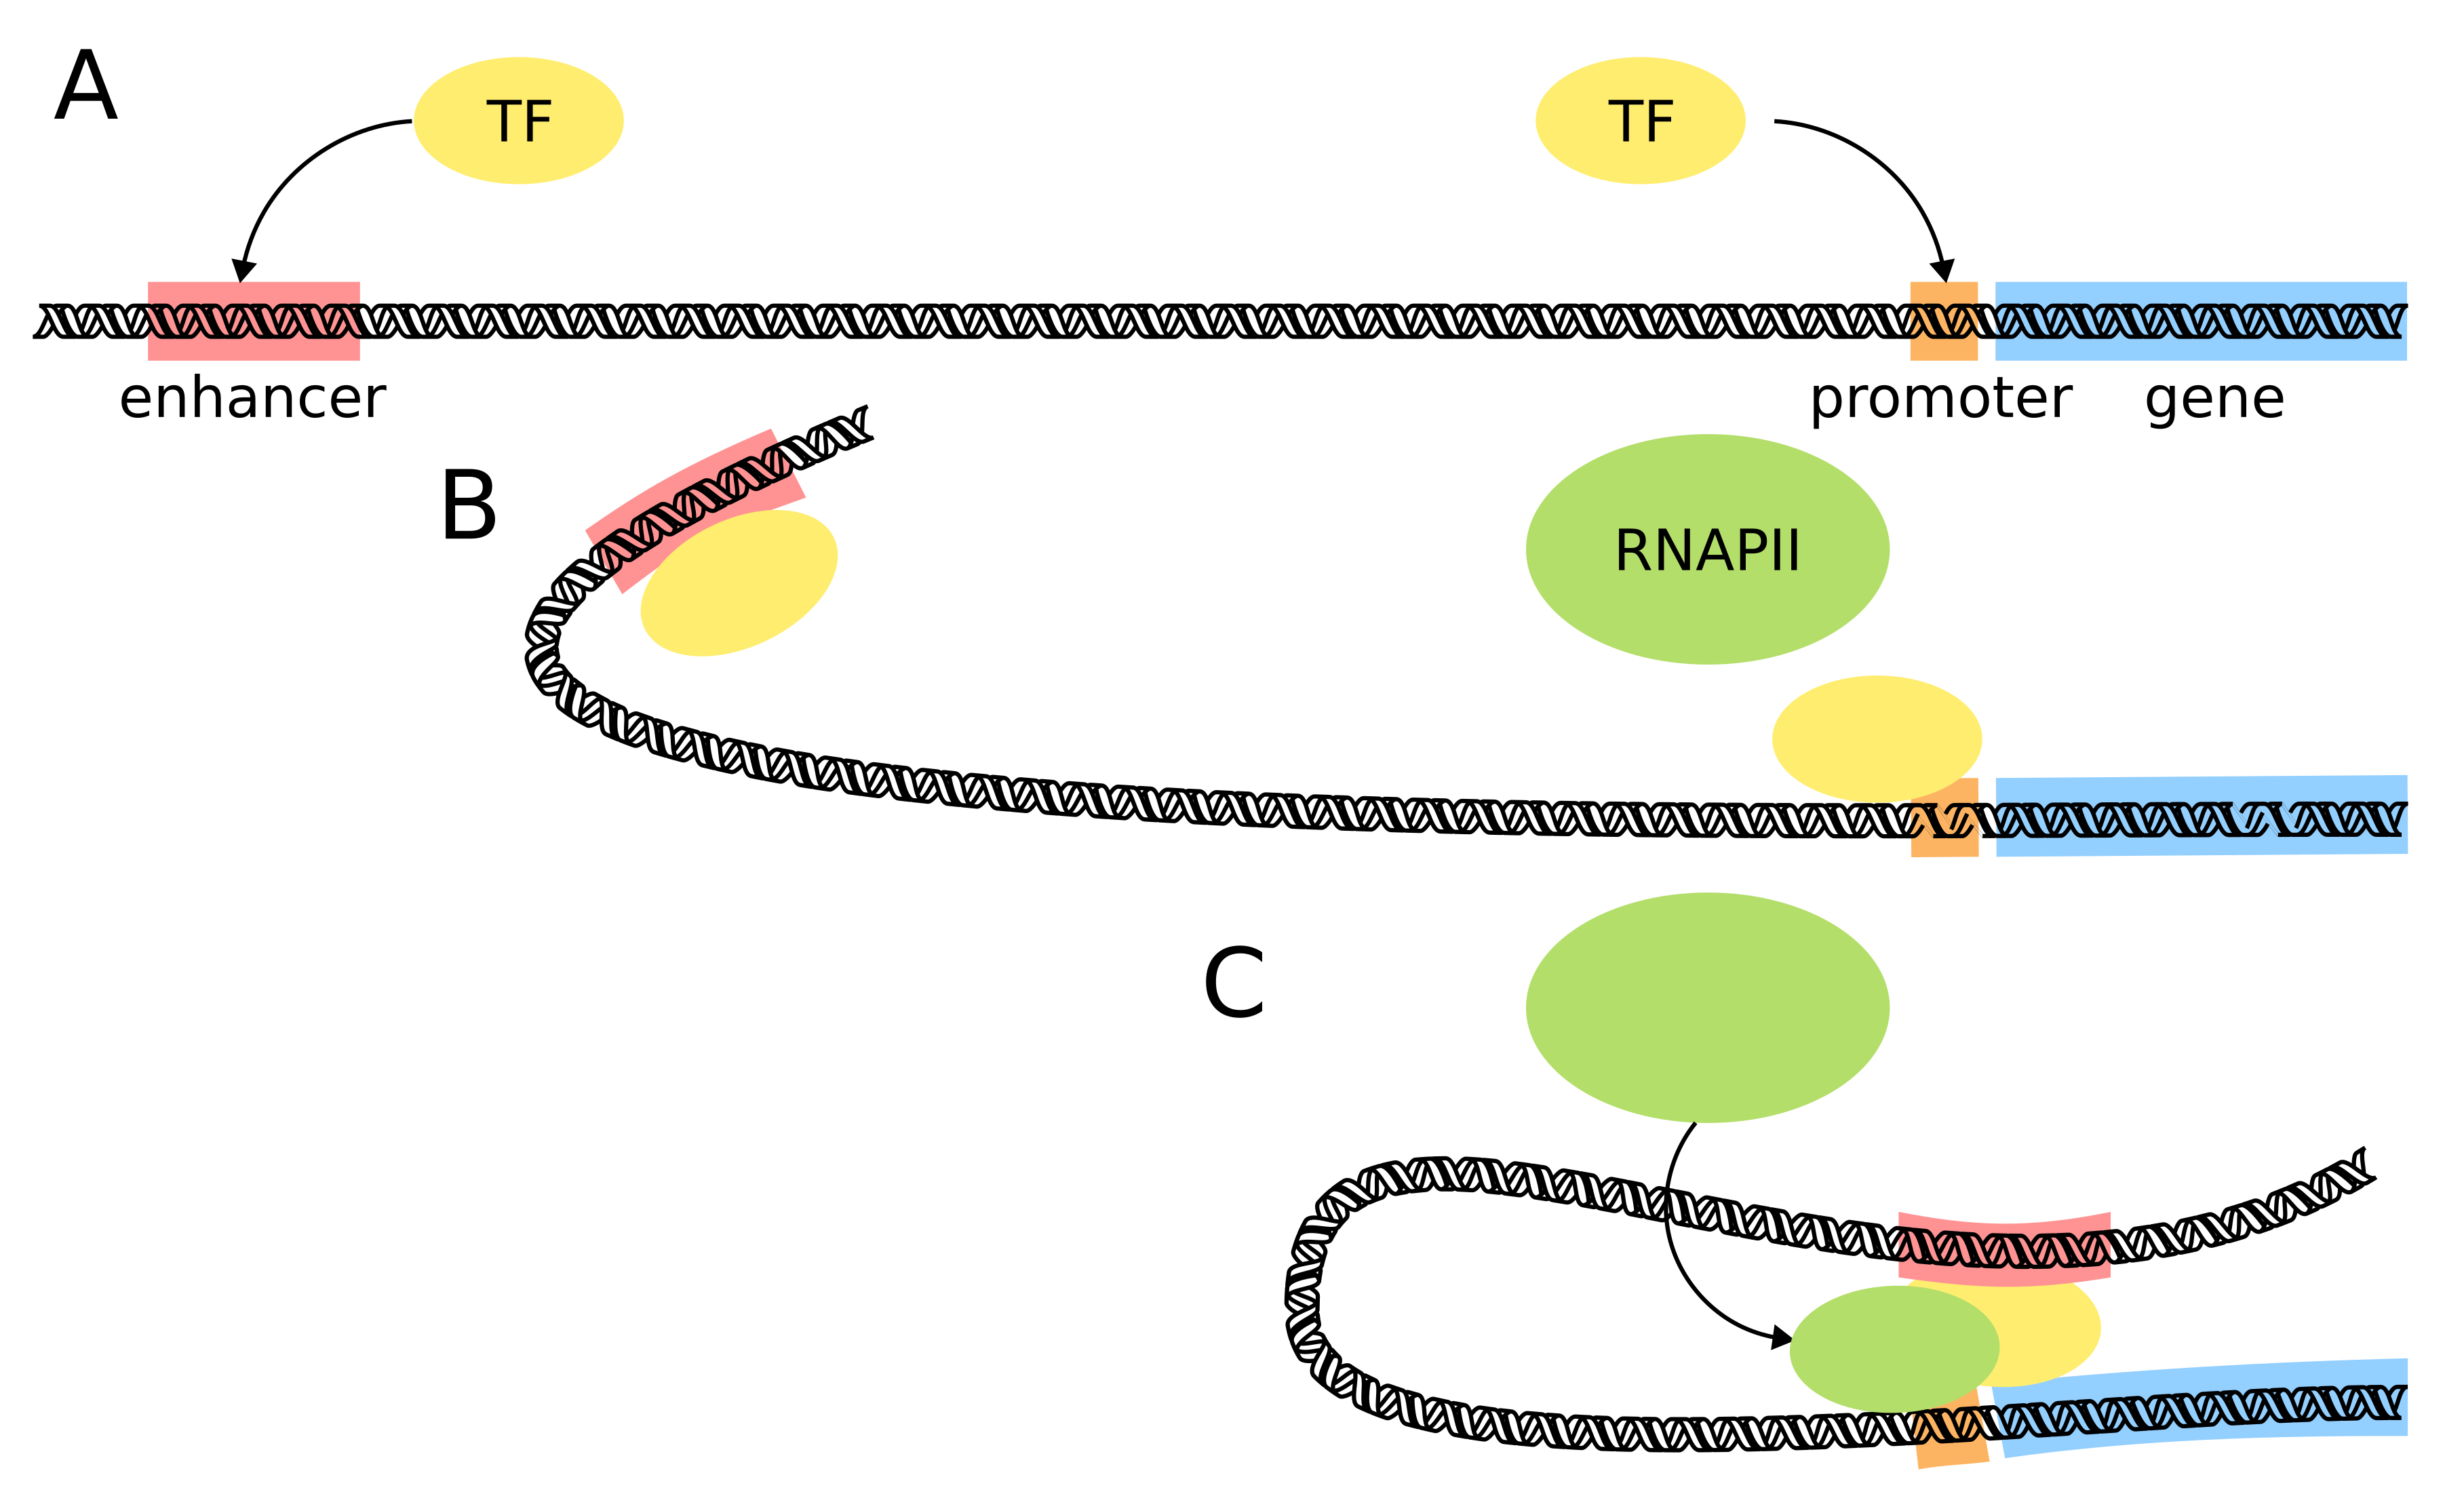
\includegraphics[width=\linewidth]{ch1.Introduction/imgs/transcription_factor.png}
    \caption{Caption}
    \label{fig:TF}
\end{figure}

\subsection{Chromatin context}

To fit 2 meters of DNA fold it

\begin{figure}[H]
    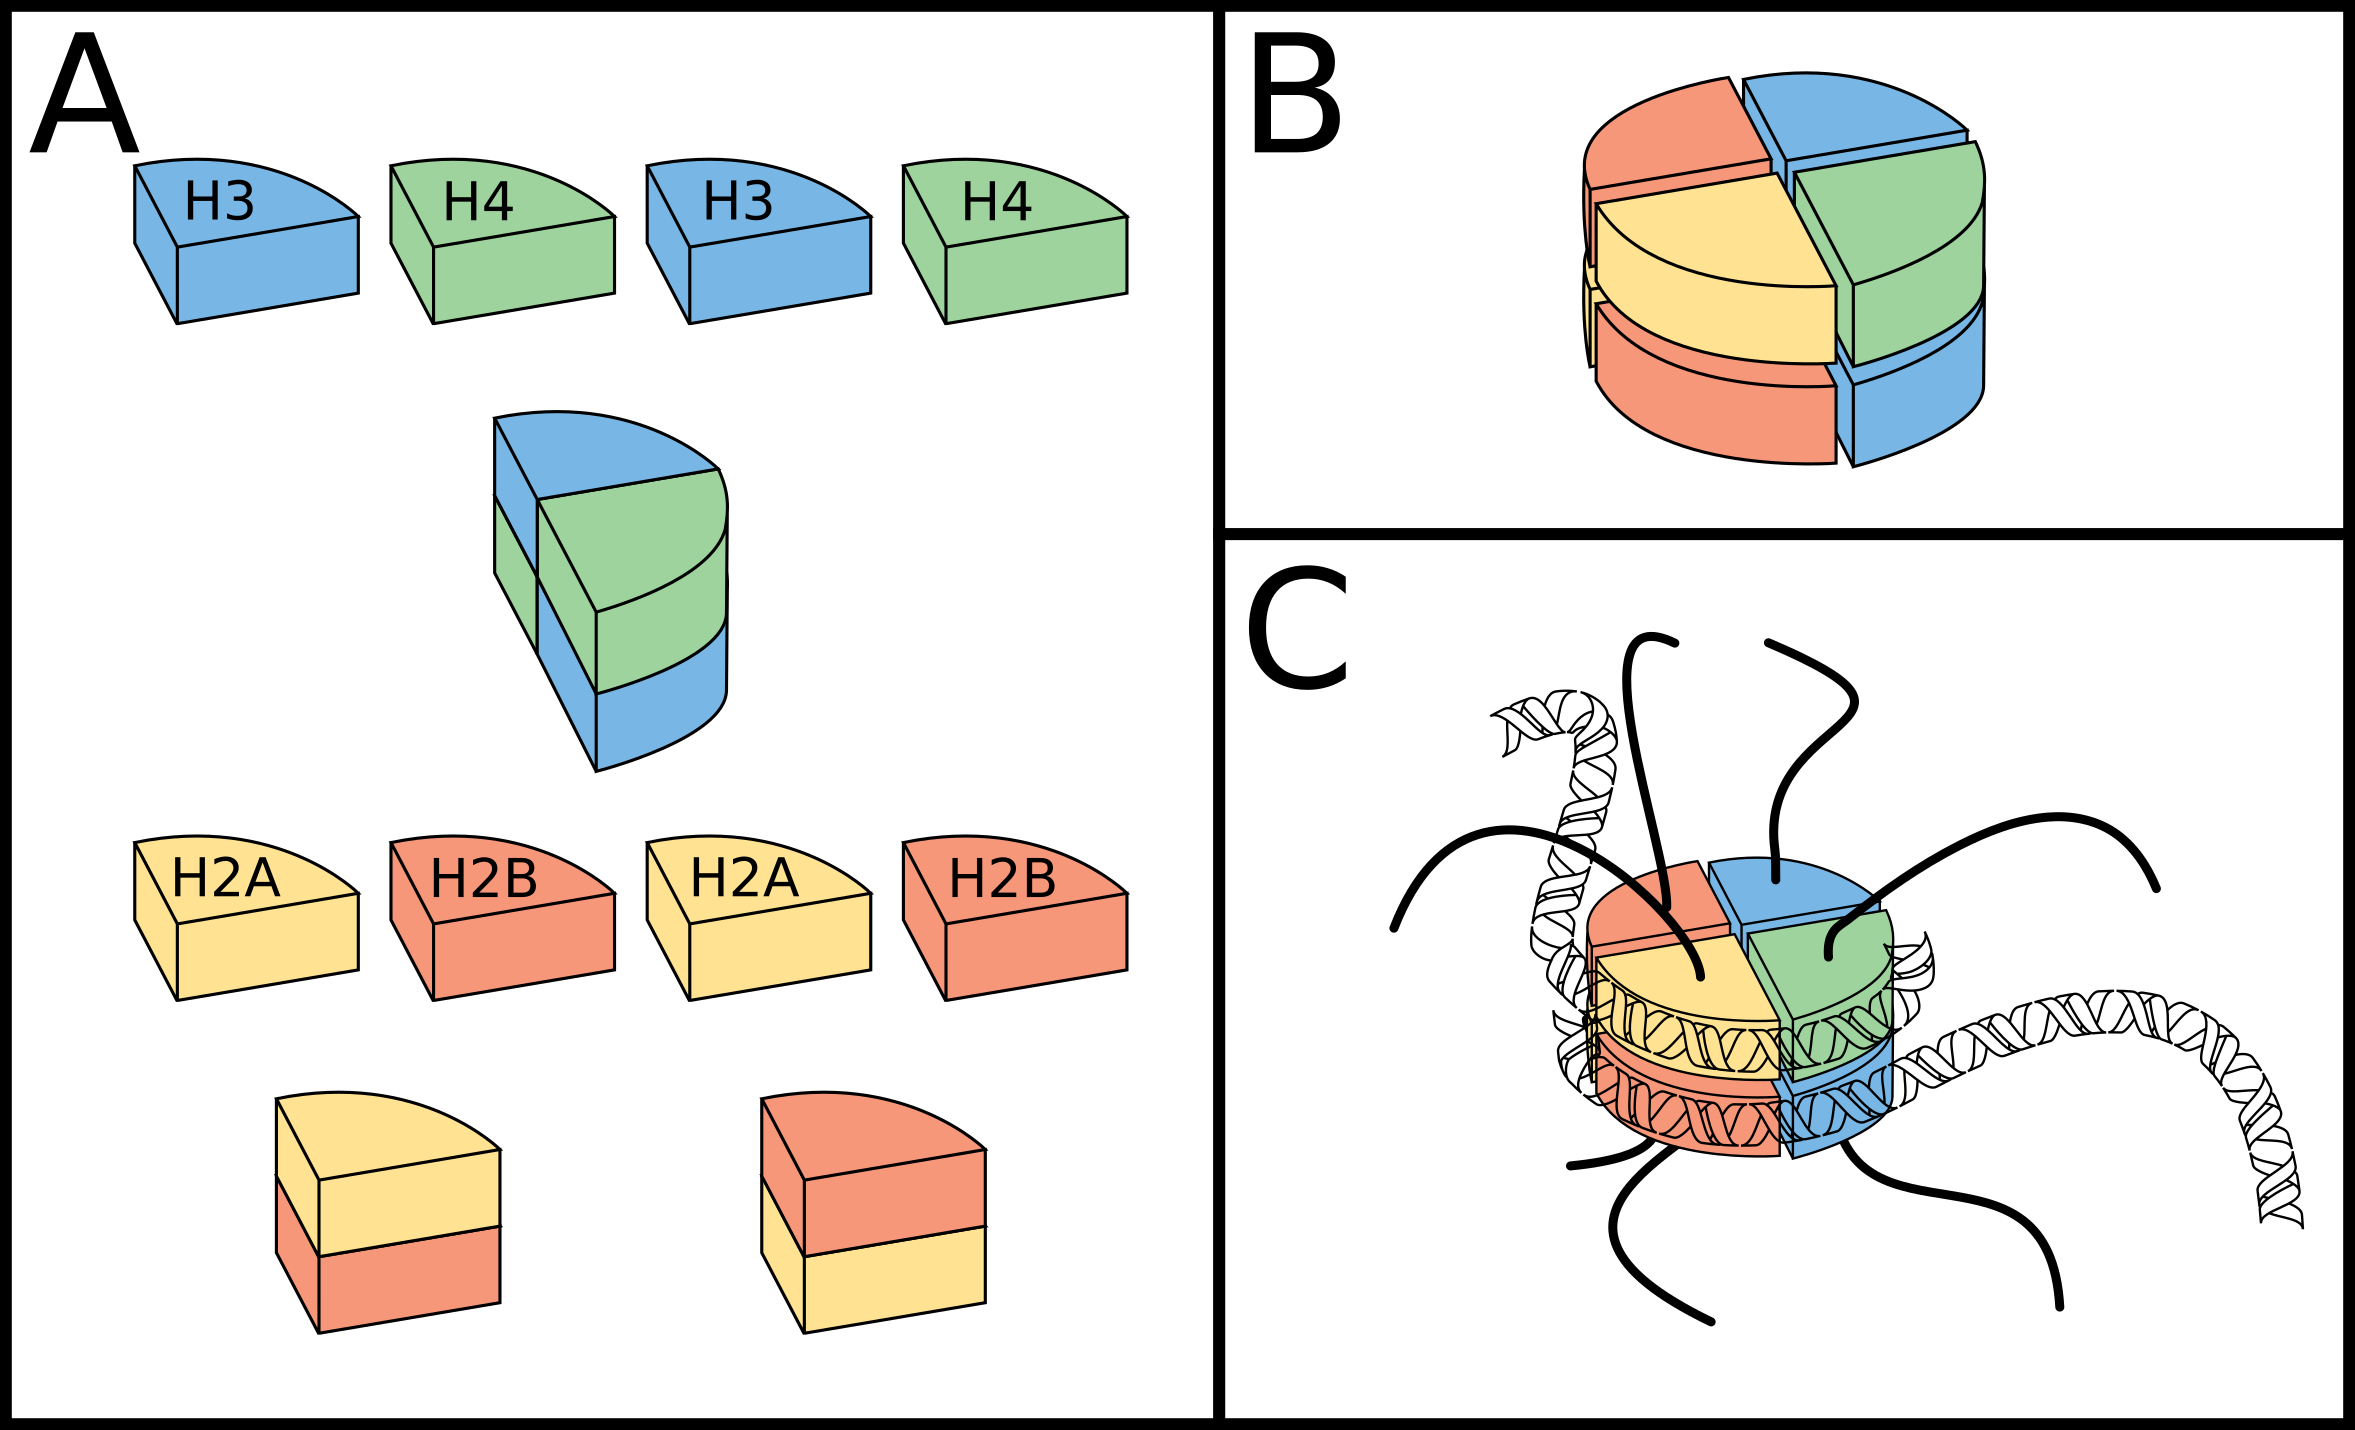
\includegraphics[width=\linewidth]{ch1.Introduction/imgs/histones.png}
    \caption{Caption}
    \label{fig:histones}
\end{figure}

should there be text here?

% \hvFloat[doublePage,capWidth=n,
% capPos=right,capVPos=top,bindCorr=0.0cm]{figure}
% {\includegraphics[width=1.9\textwidth]
% {ch1.Introduction/imgs/accessibility_horizontal.png}}
% [accessibility schematic overview]
% {TODO caption}{fig:accessibility}
\hvFloat[doublePage,sameHeight]%
    {figure}%
    {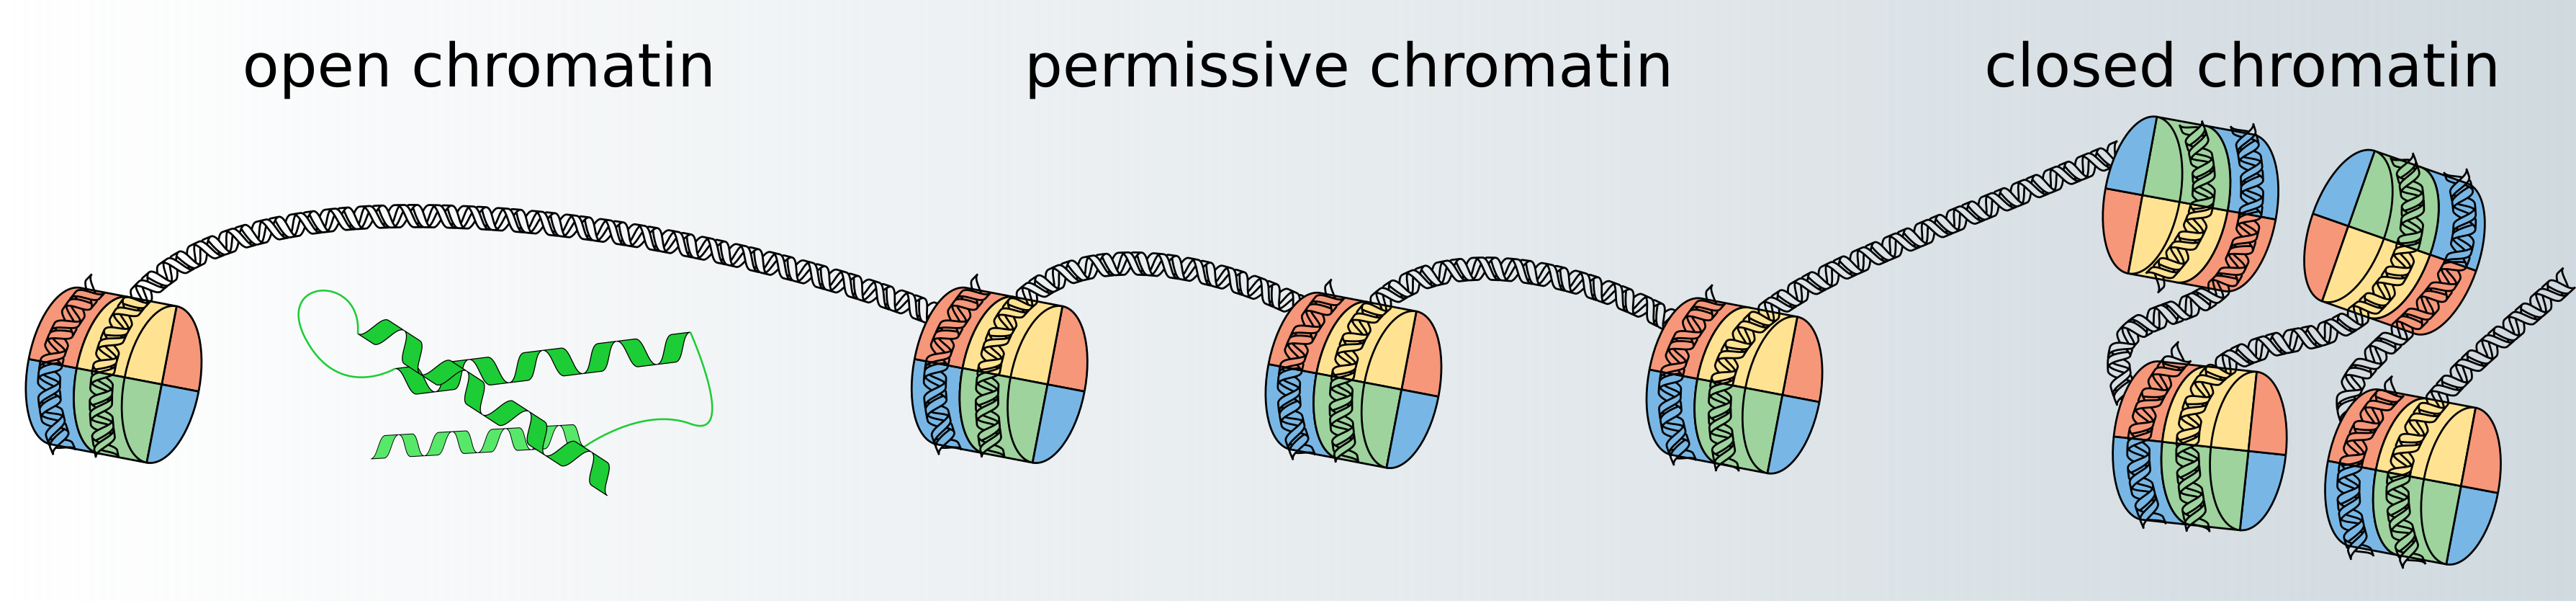
\includegraphics[doublefullPage]{ch1.Introduction/imgs/accessibility_horizontal.png}}%
    [A doublepage image with a caption on the right side of the right part.]%
    {A caption for a double-sided image that will be placed on the right side of the
    right-hand part of the illustration. The illustration begins on the left edge of
    the paper. A short form is used for the LOF.
    The parameter is \texttt{doublePage}}%
    {fig:doublePage0sH}
should there be text here?

\subsection{Other gene regulatory modes}
% \subsubsection{mRNA degradation}
% \subsubsection{Post-transcriptional modification}
% \subsubsection{RNA transport}
% \subsubsection{Signal transduction}

\subsection{Gene regulatory networks}

Mapping the relationship between genes is crucial for understanding how cellular processes are regulated. A common abstraction to understand gene-gene interactions are gene regulatory networks.  

The first gene regulatory network was proposed by Roy Britten and Eric Davidson in 1969\cite{Britten_1969}. They observed that a biological system (i) responds to an external signal; (ii) then produces its own signal as a response; (iii) transmits its own signal to receptors that do not perceive the external signal; (iv) then respond to its own signal, and finally (v) produces a protein as a response. Without modern knowledge of gene regulation, they then correctly reverse-engineered what the minimum requirements are for such a system. One of the things they then predicted was the existence of transcription factors and promoter sequences. It took Eric Davidson more than 30 years to experimentally validate his original work\cite{Davidson_2002}.

Gene regulatory networks are often modeled and visualized with direct gene-gene interactions (fig. \ref{fig:network}A). This means for instance that the protein product of gene $\alpha$ directly regulates the protein product of gene $\beta$, ignoring all steps in between. Even though this is a gross oversimplification of gene-gene interactions, these simple models can already exhibit complex behavior. One of the older and well-known examples of this complex behavior are Turing patterns, discovered by the famous computer scientist Alan Turing\cite{Turing1952}. We consider a system of two genes, gene $\alpha$ and gene $\beta$, where gene $\alpha$ upregulates itself and gene $\beta$, but gene $\beta$ inhibits gene $\alpha$ (fig. \ref{fig:network}B). When modeling this simple two-gene network in a spatial setting it produces complex patterns (fig. \ref{fig:network}C), of which similar patterns can be observed in nature (fig. \ref{fig:network}D).

\begin{figure}[H]
    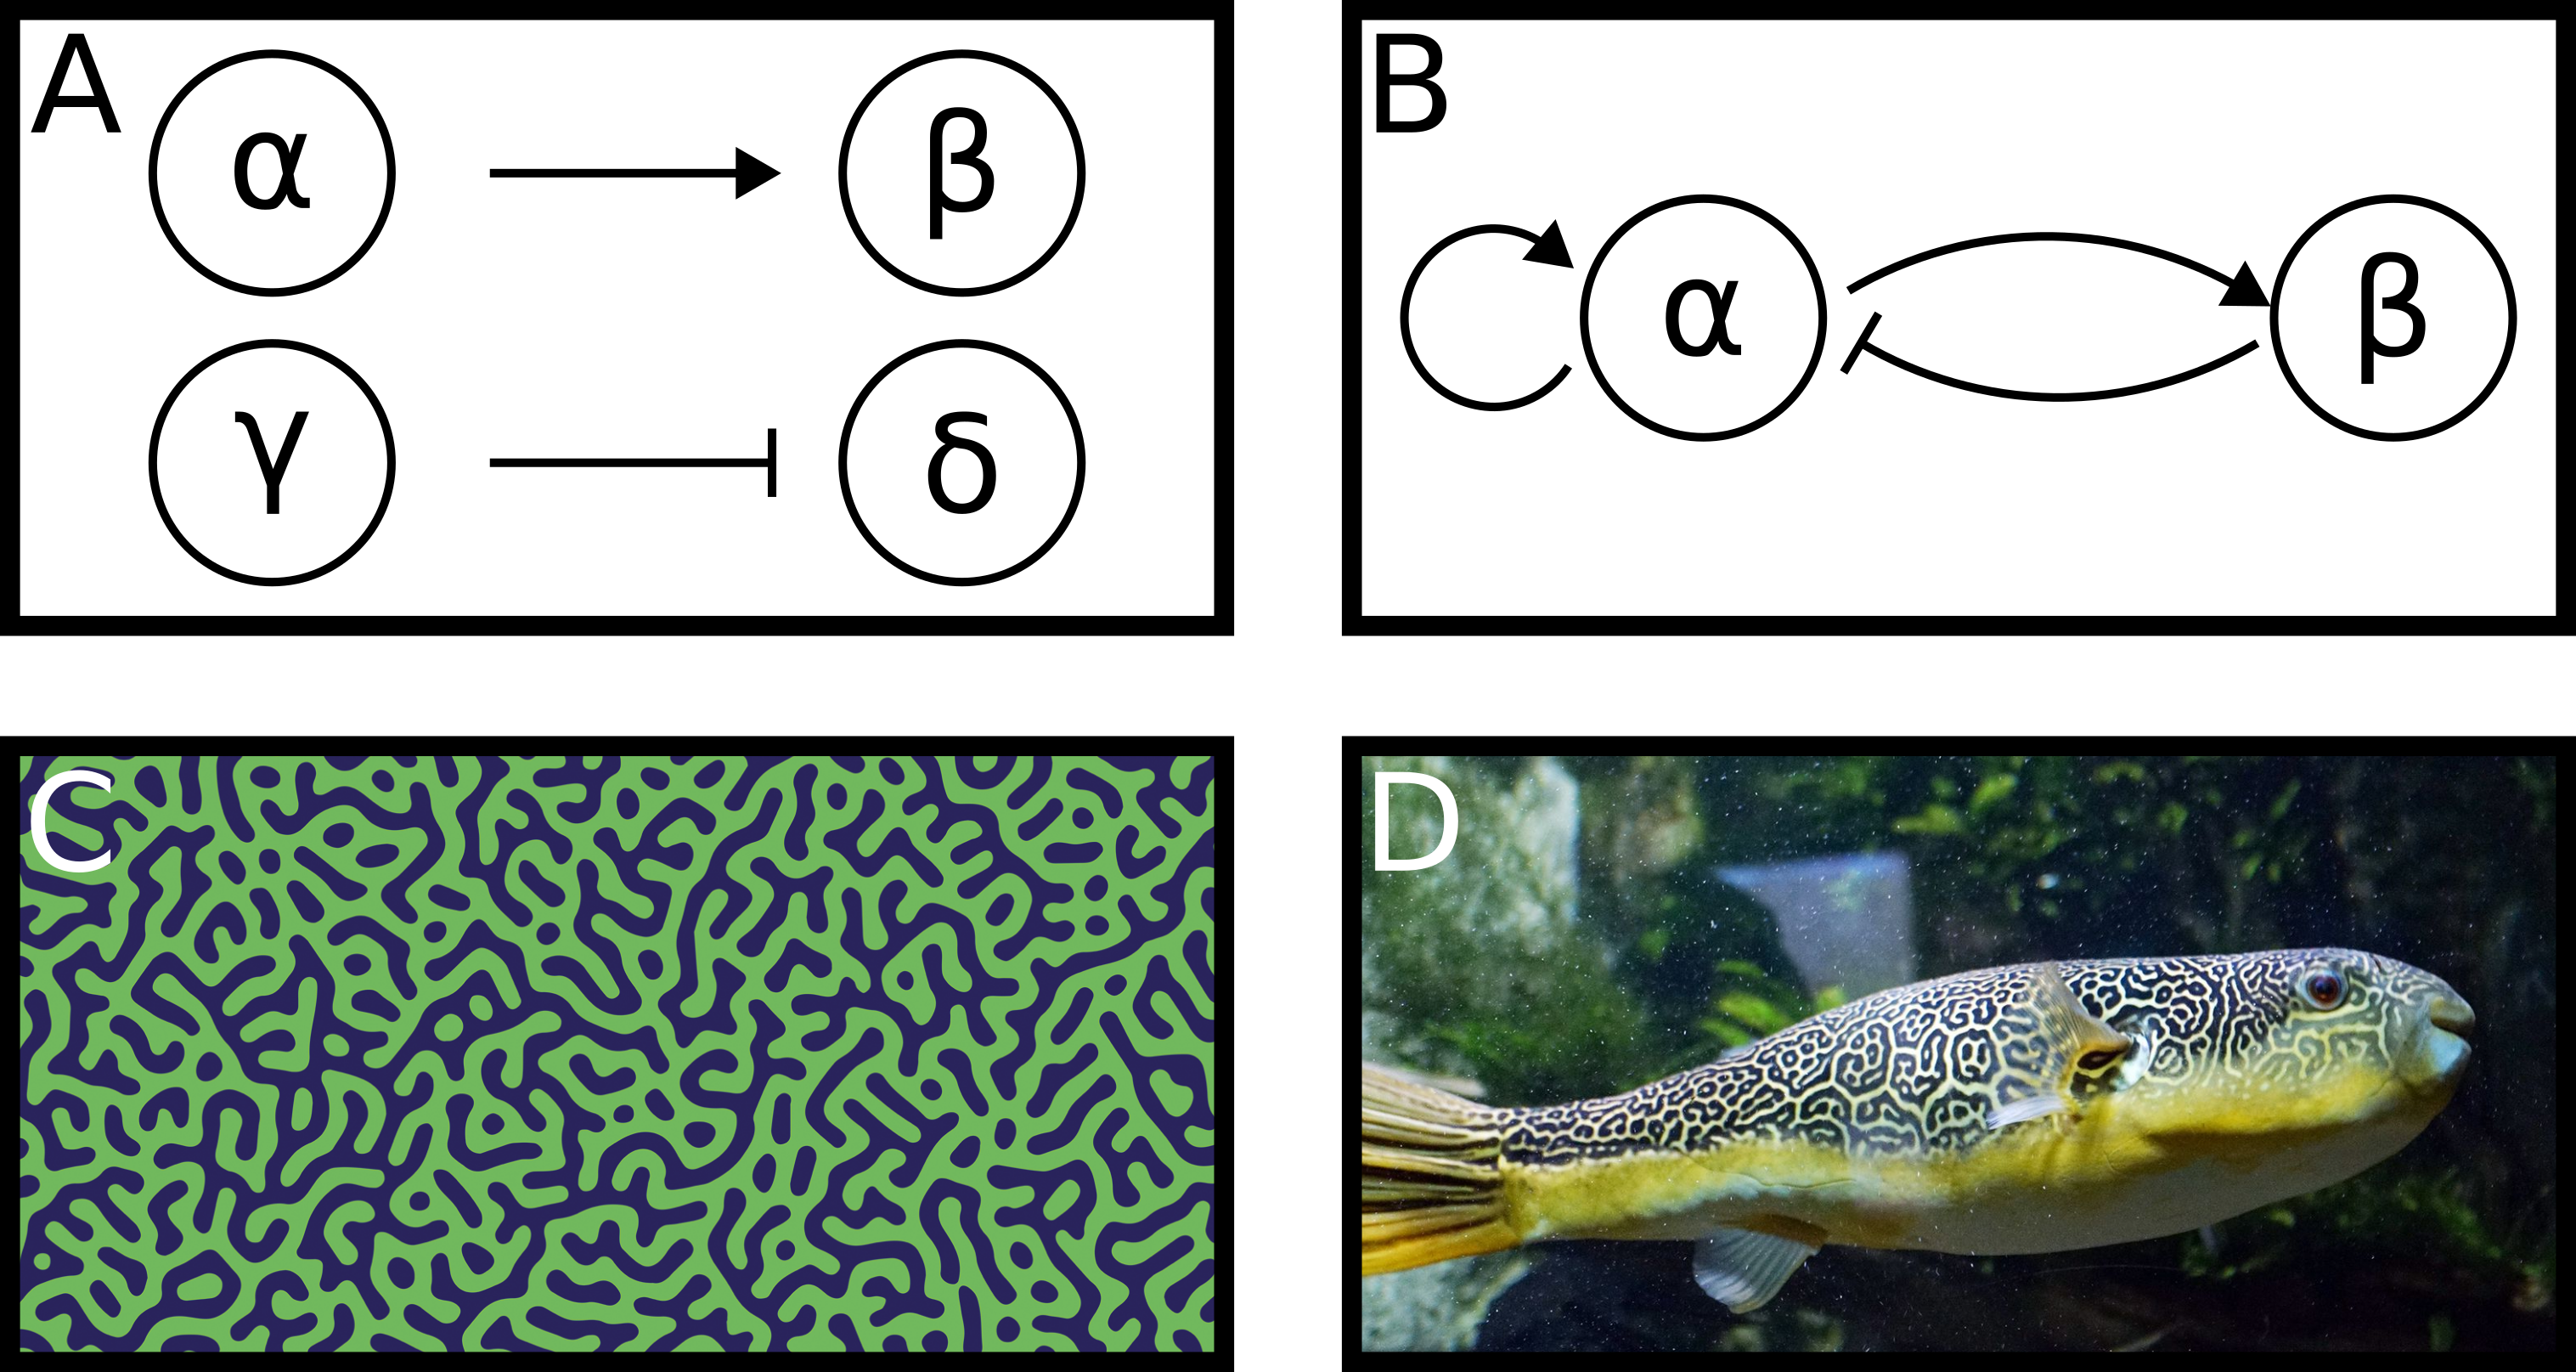
\includegraphics[width=\linewidth]{ch1.Introduction/imgs/network.png}
    \caption{(\textbf{A}) standard way of representing gene-gene interactions. Gene $\alpha$ upregulates gene $\beta$, and gene $\gamma$ downregulates gene $\delta$. (\textbf{B}) Gierer-Meinhardt gene regulatory network, where gene $\alpha$ upregulates itself and gene $\beta$, and gene $\beta$ downregulates gene $\alpha$. (\textbf{C}) Simulation of the Gierer-Meinhardt gene regulatory network in a spatial context. (\textbf{D}) A Mbuna pufferfish with Turing pattern. Image from Tiia Monto(https://en.wikipedia.org/wiki/Mbu\_pufferfish\#/media/File:Tetraodon\_mbu\_2.jpg)}
    \label{fig:network}
\end{figure}

TODO more recent / complex gene networks. 

\section{Evolutionary development (evo-devo)}

A single fertilized egg cell develops into a complex collection of trillions of cells by the time the individual reaches adulthood. All the information necessary for this development is present at fertilization. How does each cell know what to develop into? 

In the 1980s scientists discovered 

\begin{figure}[H]
    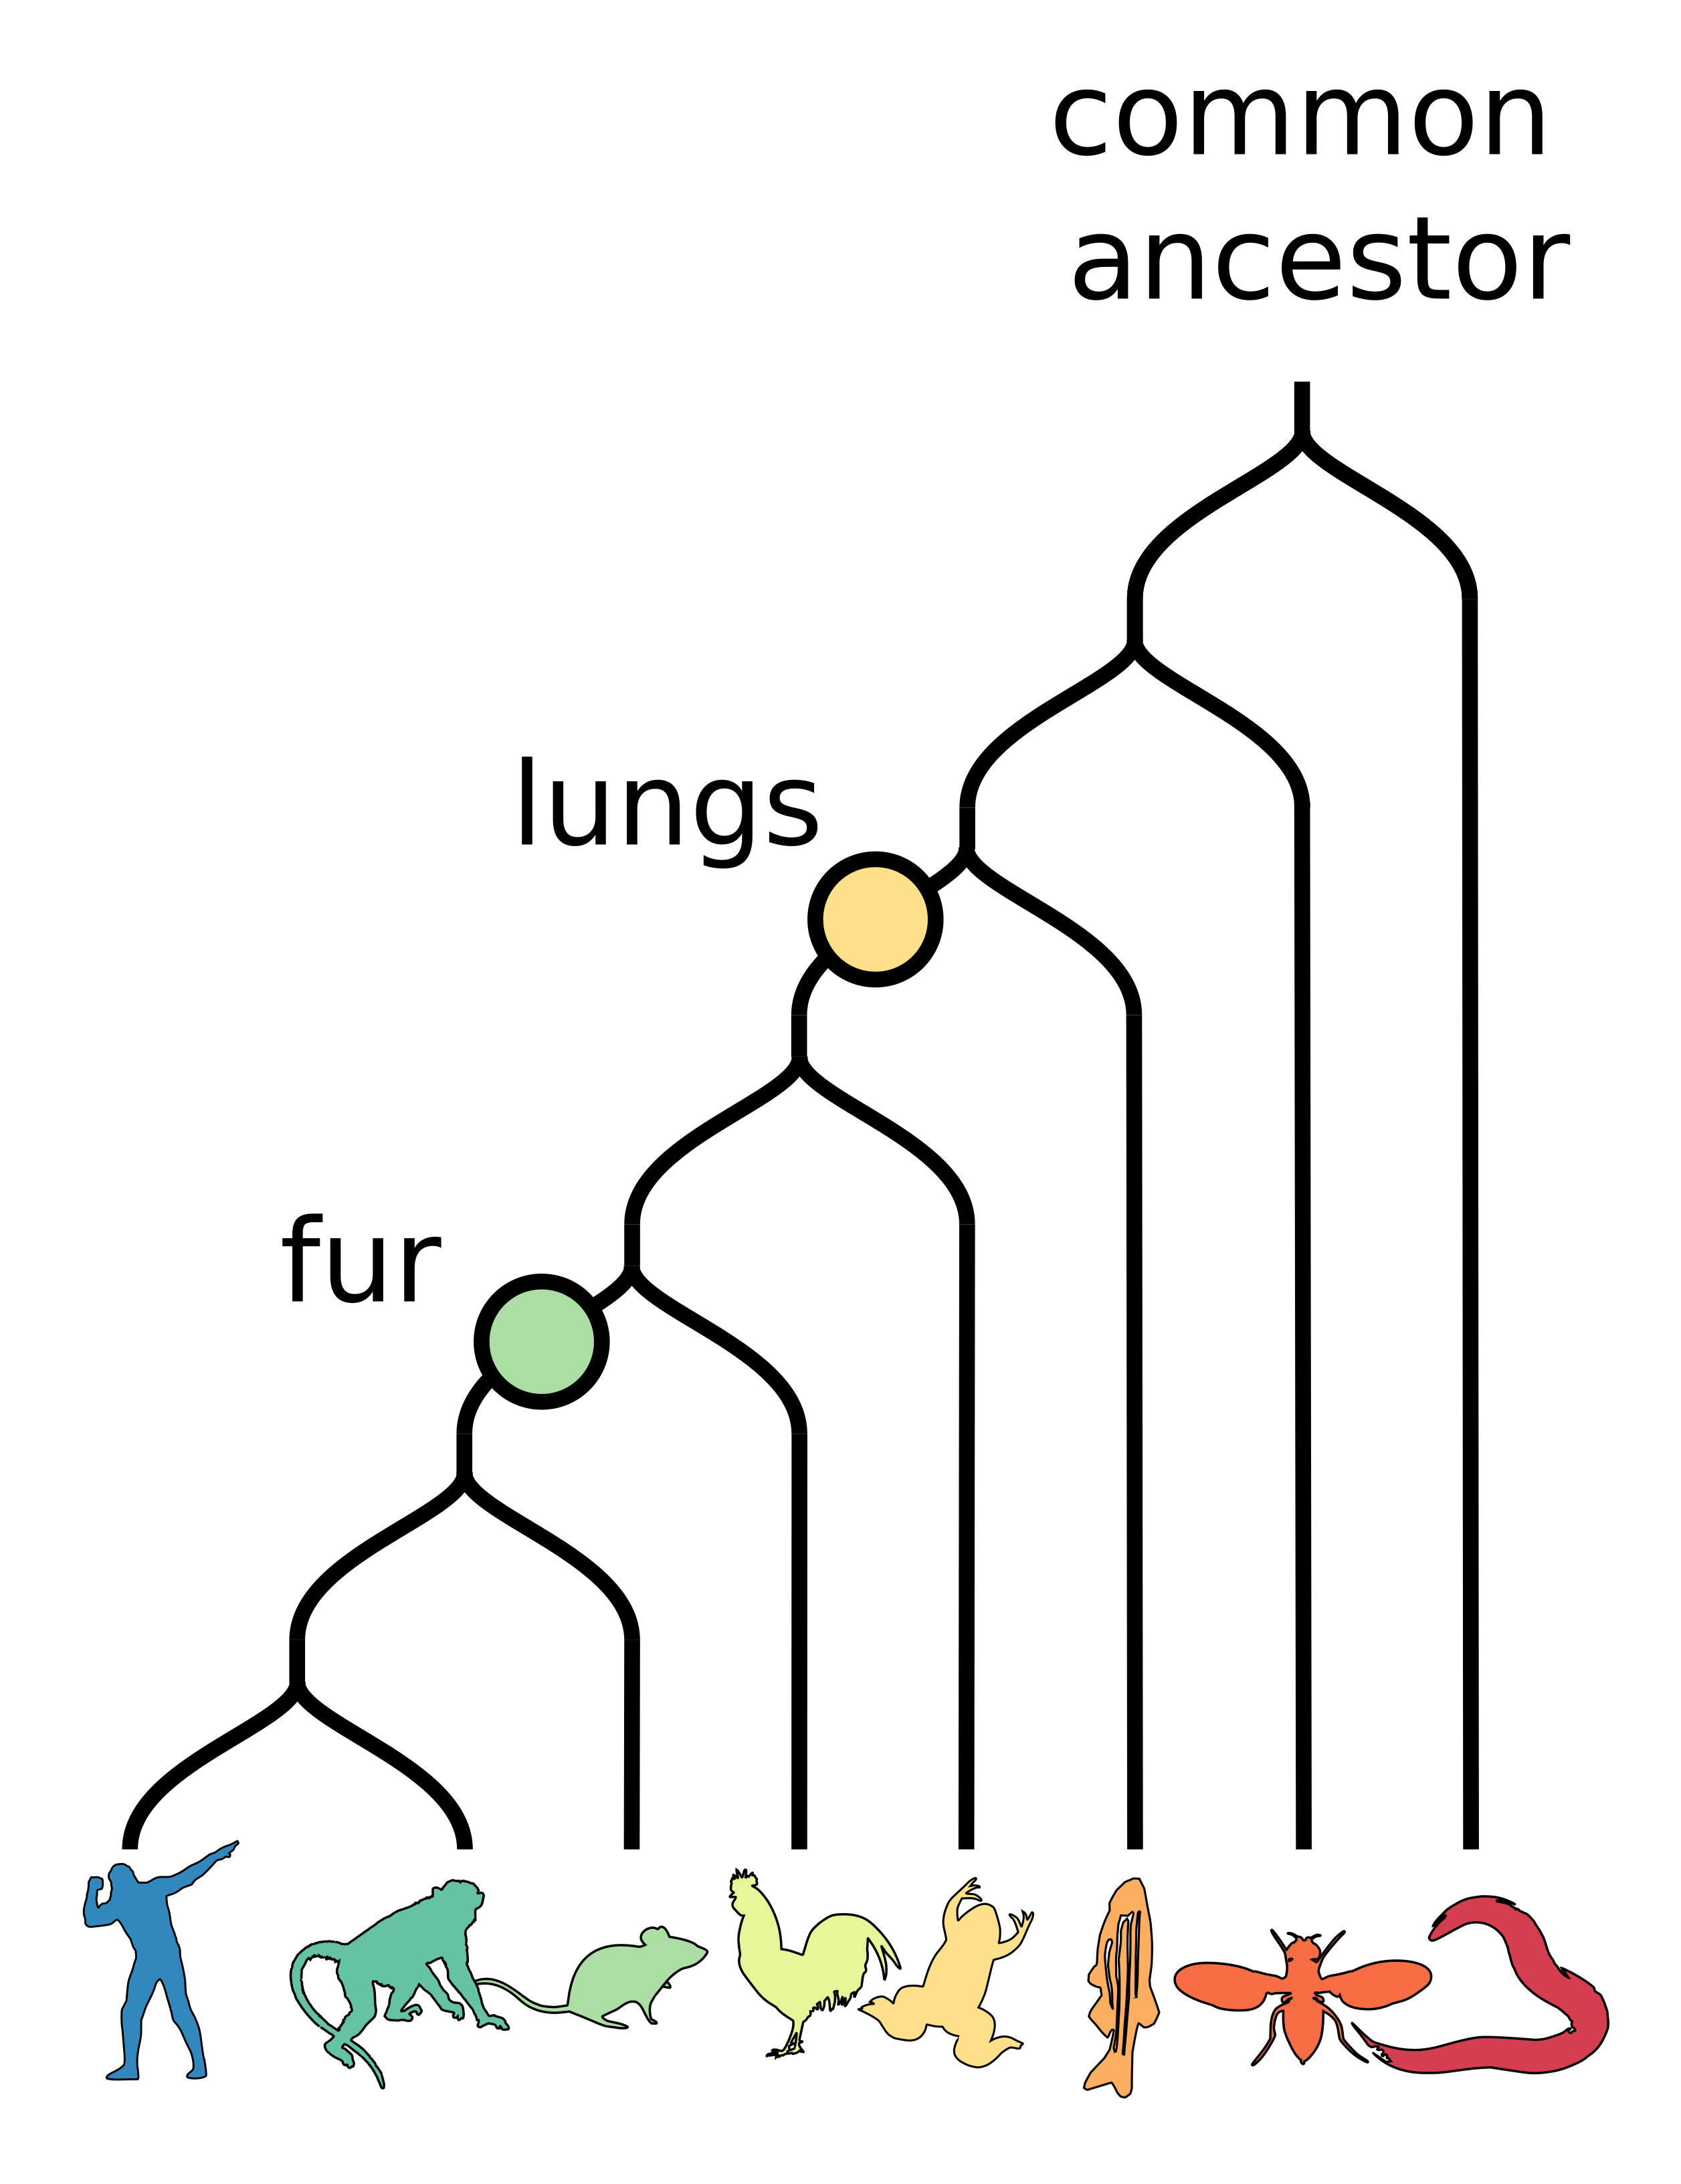
\includegraphics[width=0.5\linewidth]{ch1.Introduction/imgs/phylogeny.png}
    \caption{caption}
    \label{fig:phylogeny}
\end{figure}

\subsection{evo-devo gene toolkit}

\subsection{The hourglass model and the phylotypic stage}



\begin{figure}[H]
    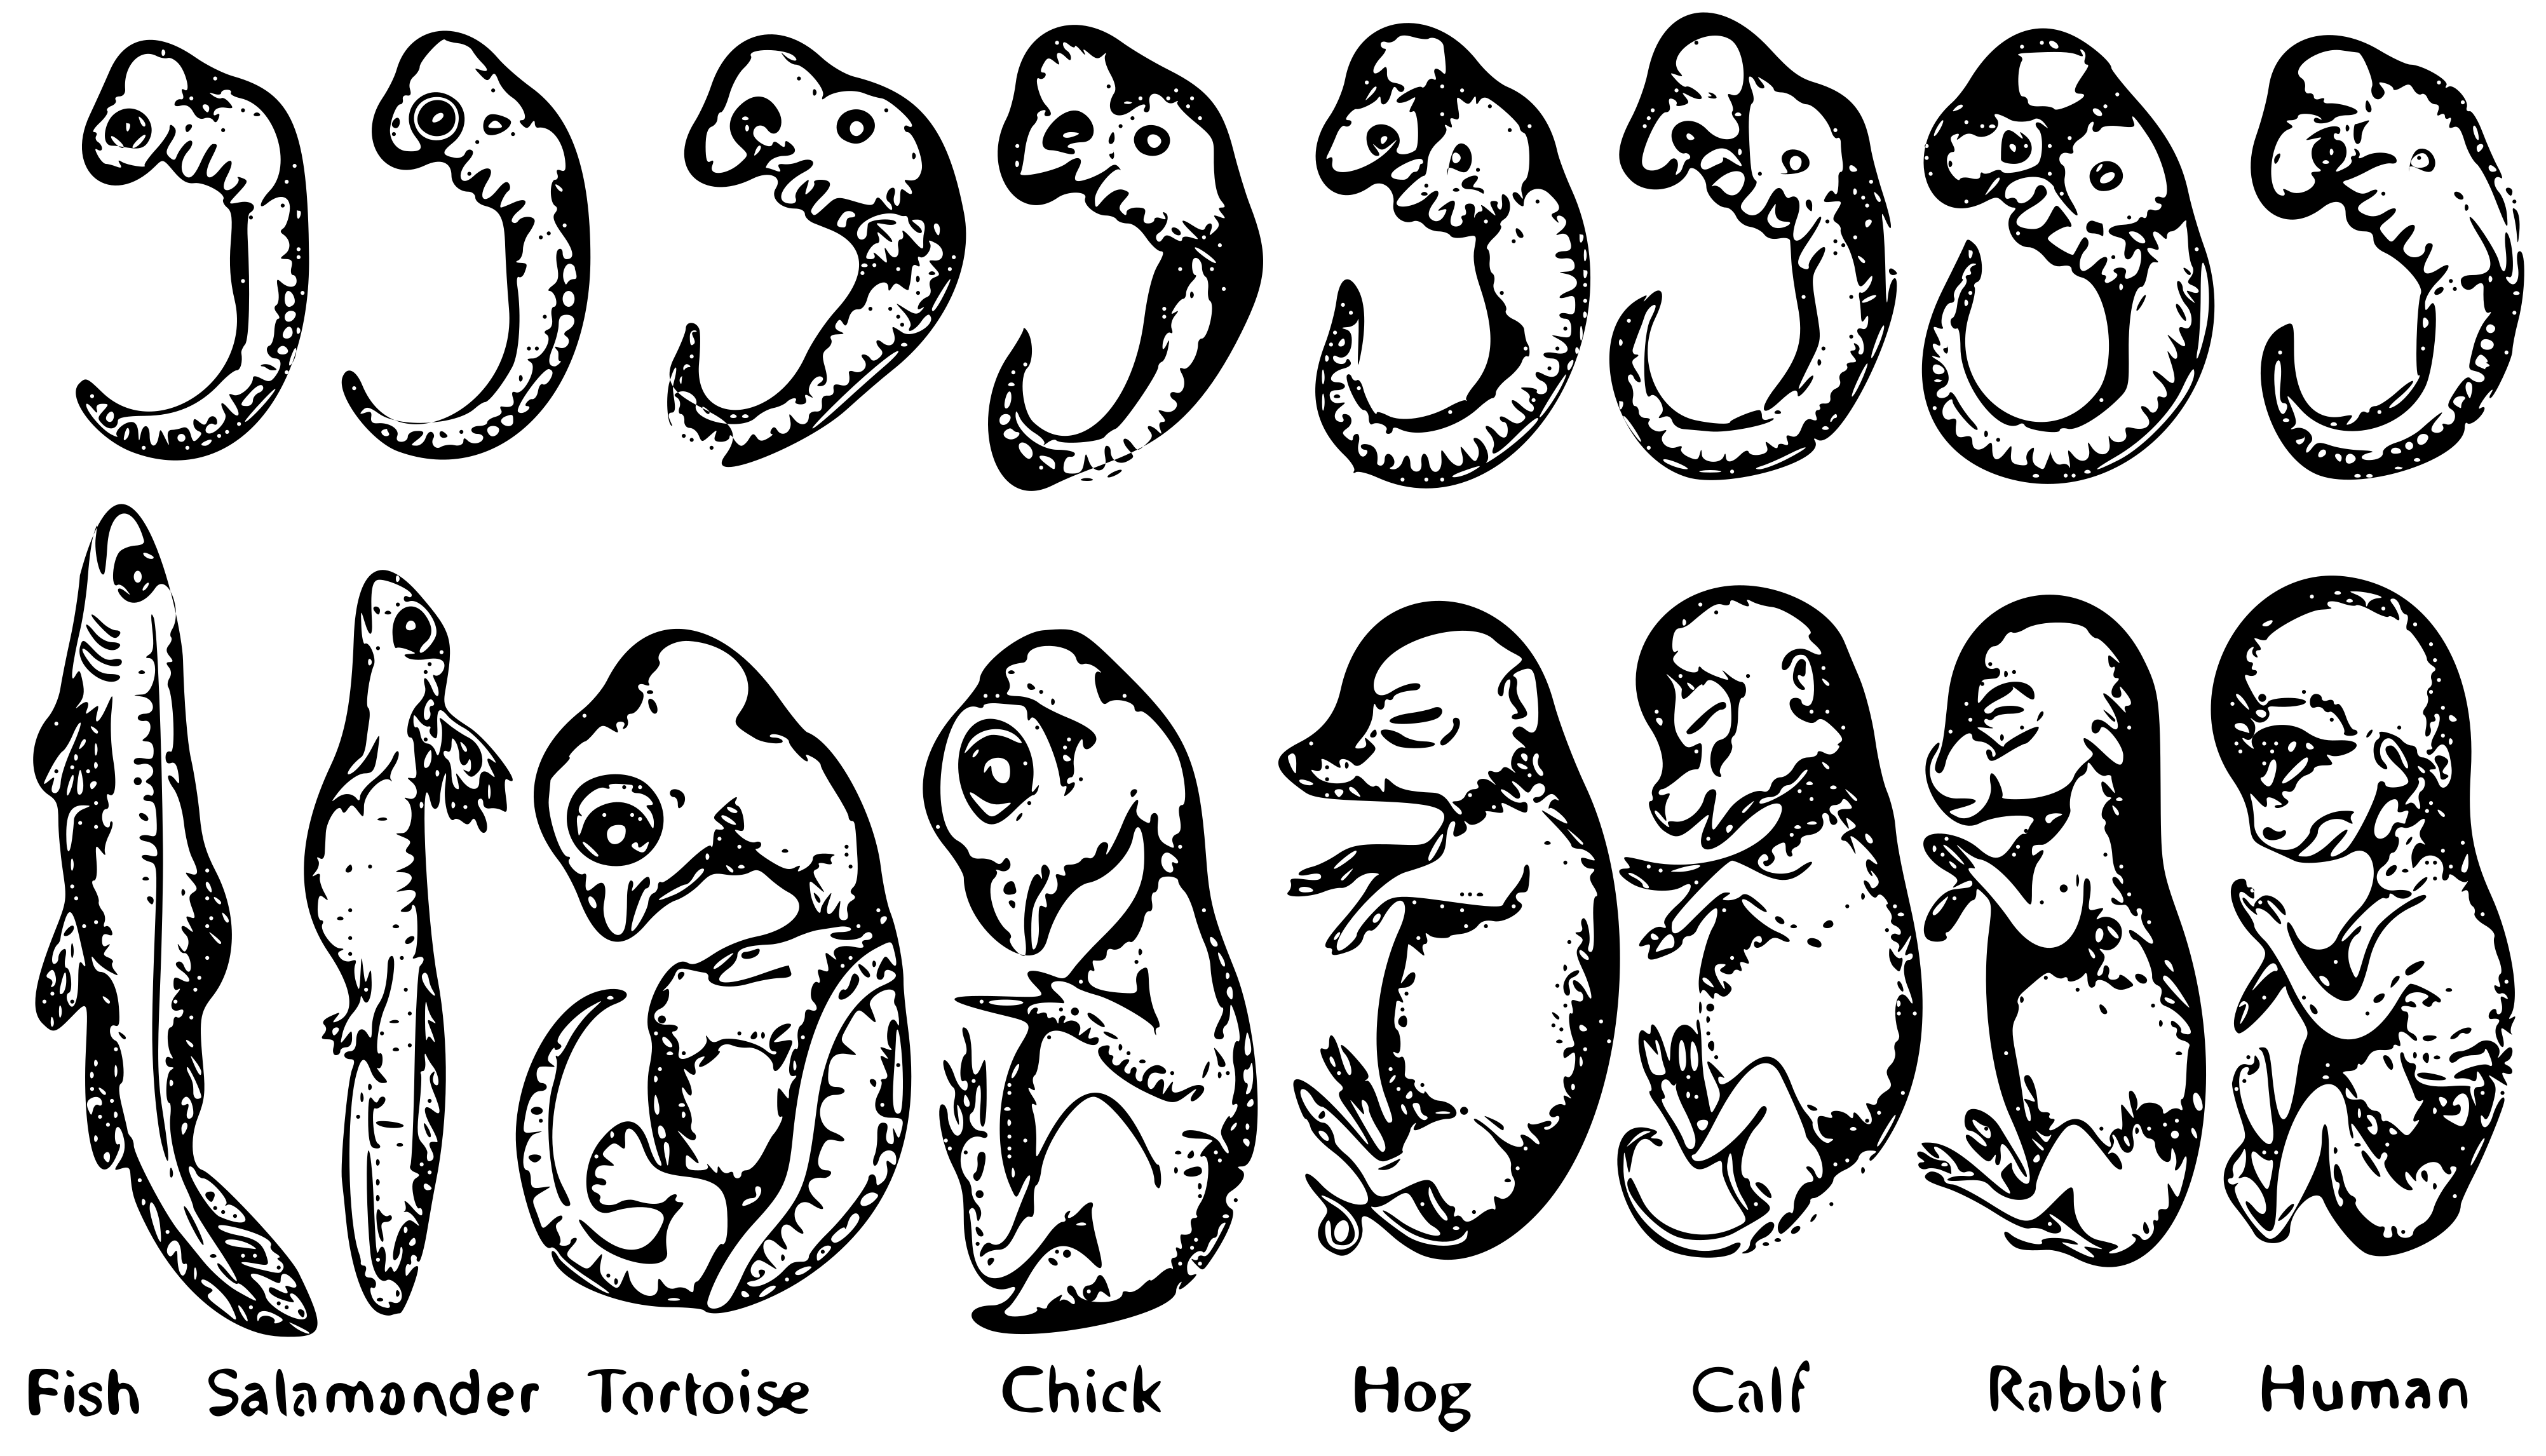
\includegraphics[width=\linewidth]{ch1.Introduction/imgs/haeckel.png}
    \caption{caption}
    \label{fig:haeckel}
\end{figure}

\begin{figure}[H]
    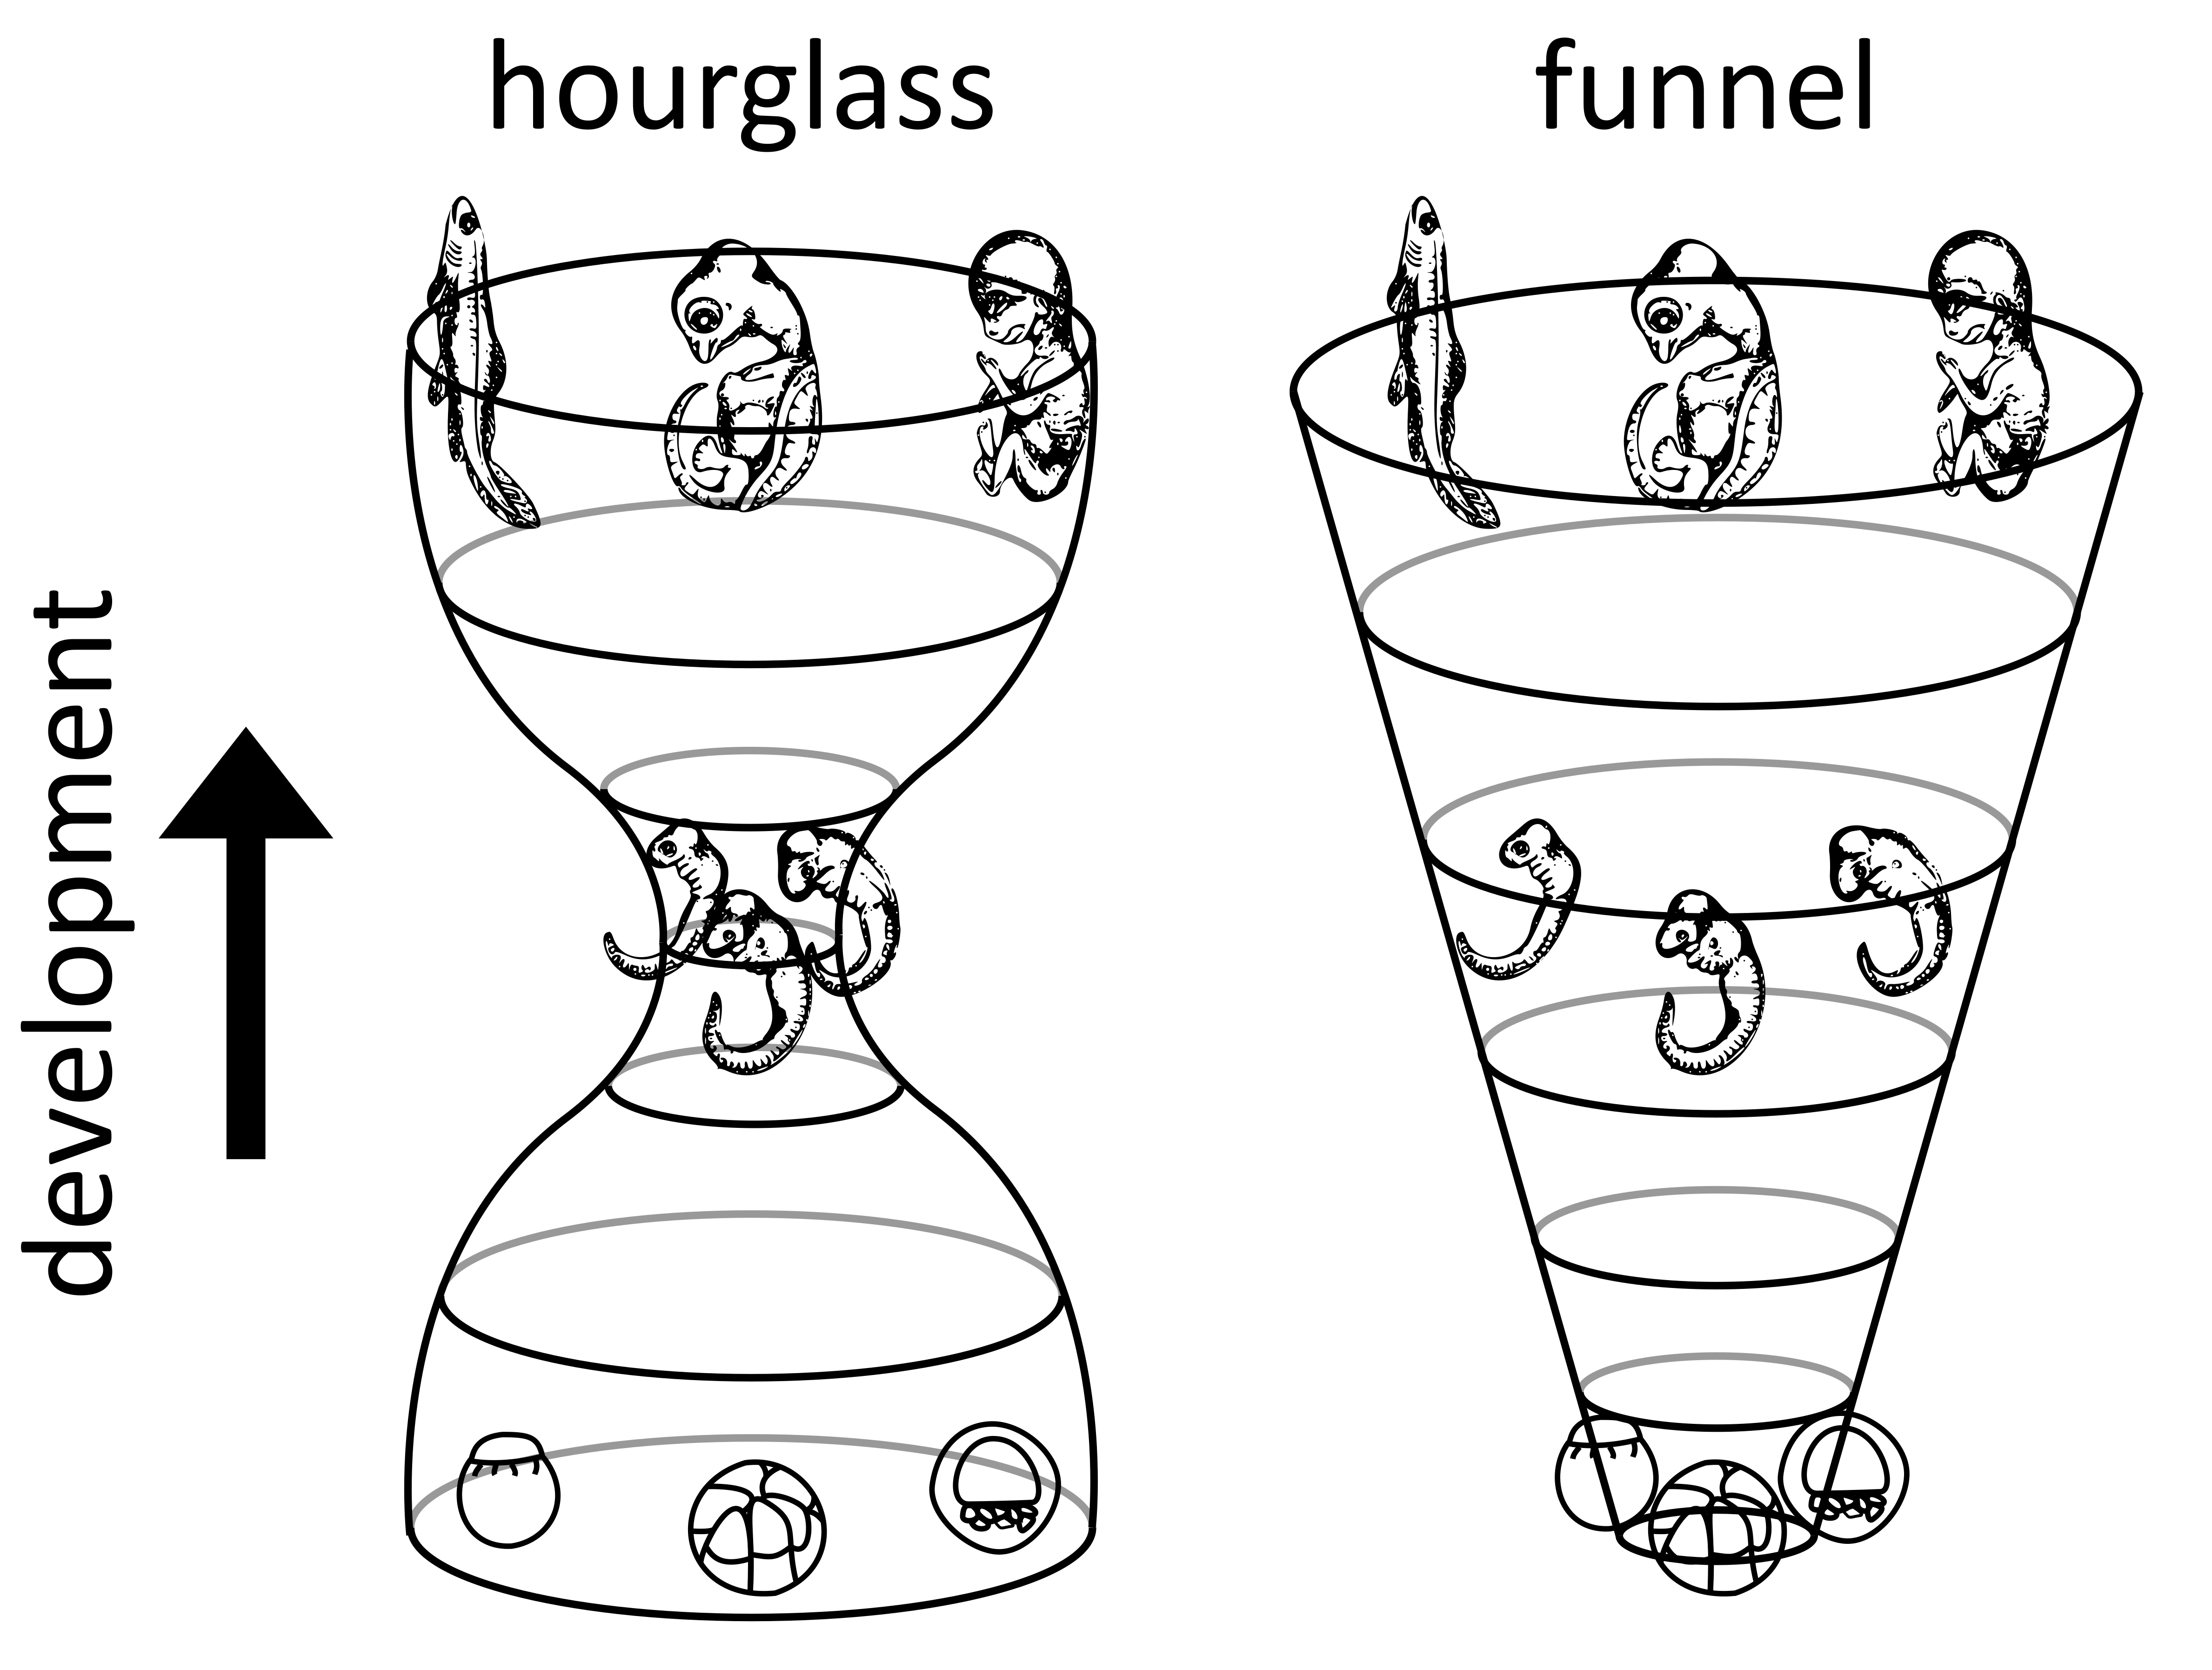
\includegraphics[width=\linewidth]{ch1.Introduction/imgs/hourglass.png}
    \caption{caption}
    \label{fig:hourglass}
\end{figure}

\section{Computational biology}

The field of computational biology concerns itself with the analysis of the enormous quantities of data that molecular biology produces. In this thesis the analysis of three different sequencing assays 

\begin{figure}[H]
    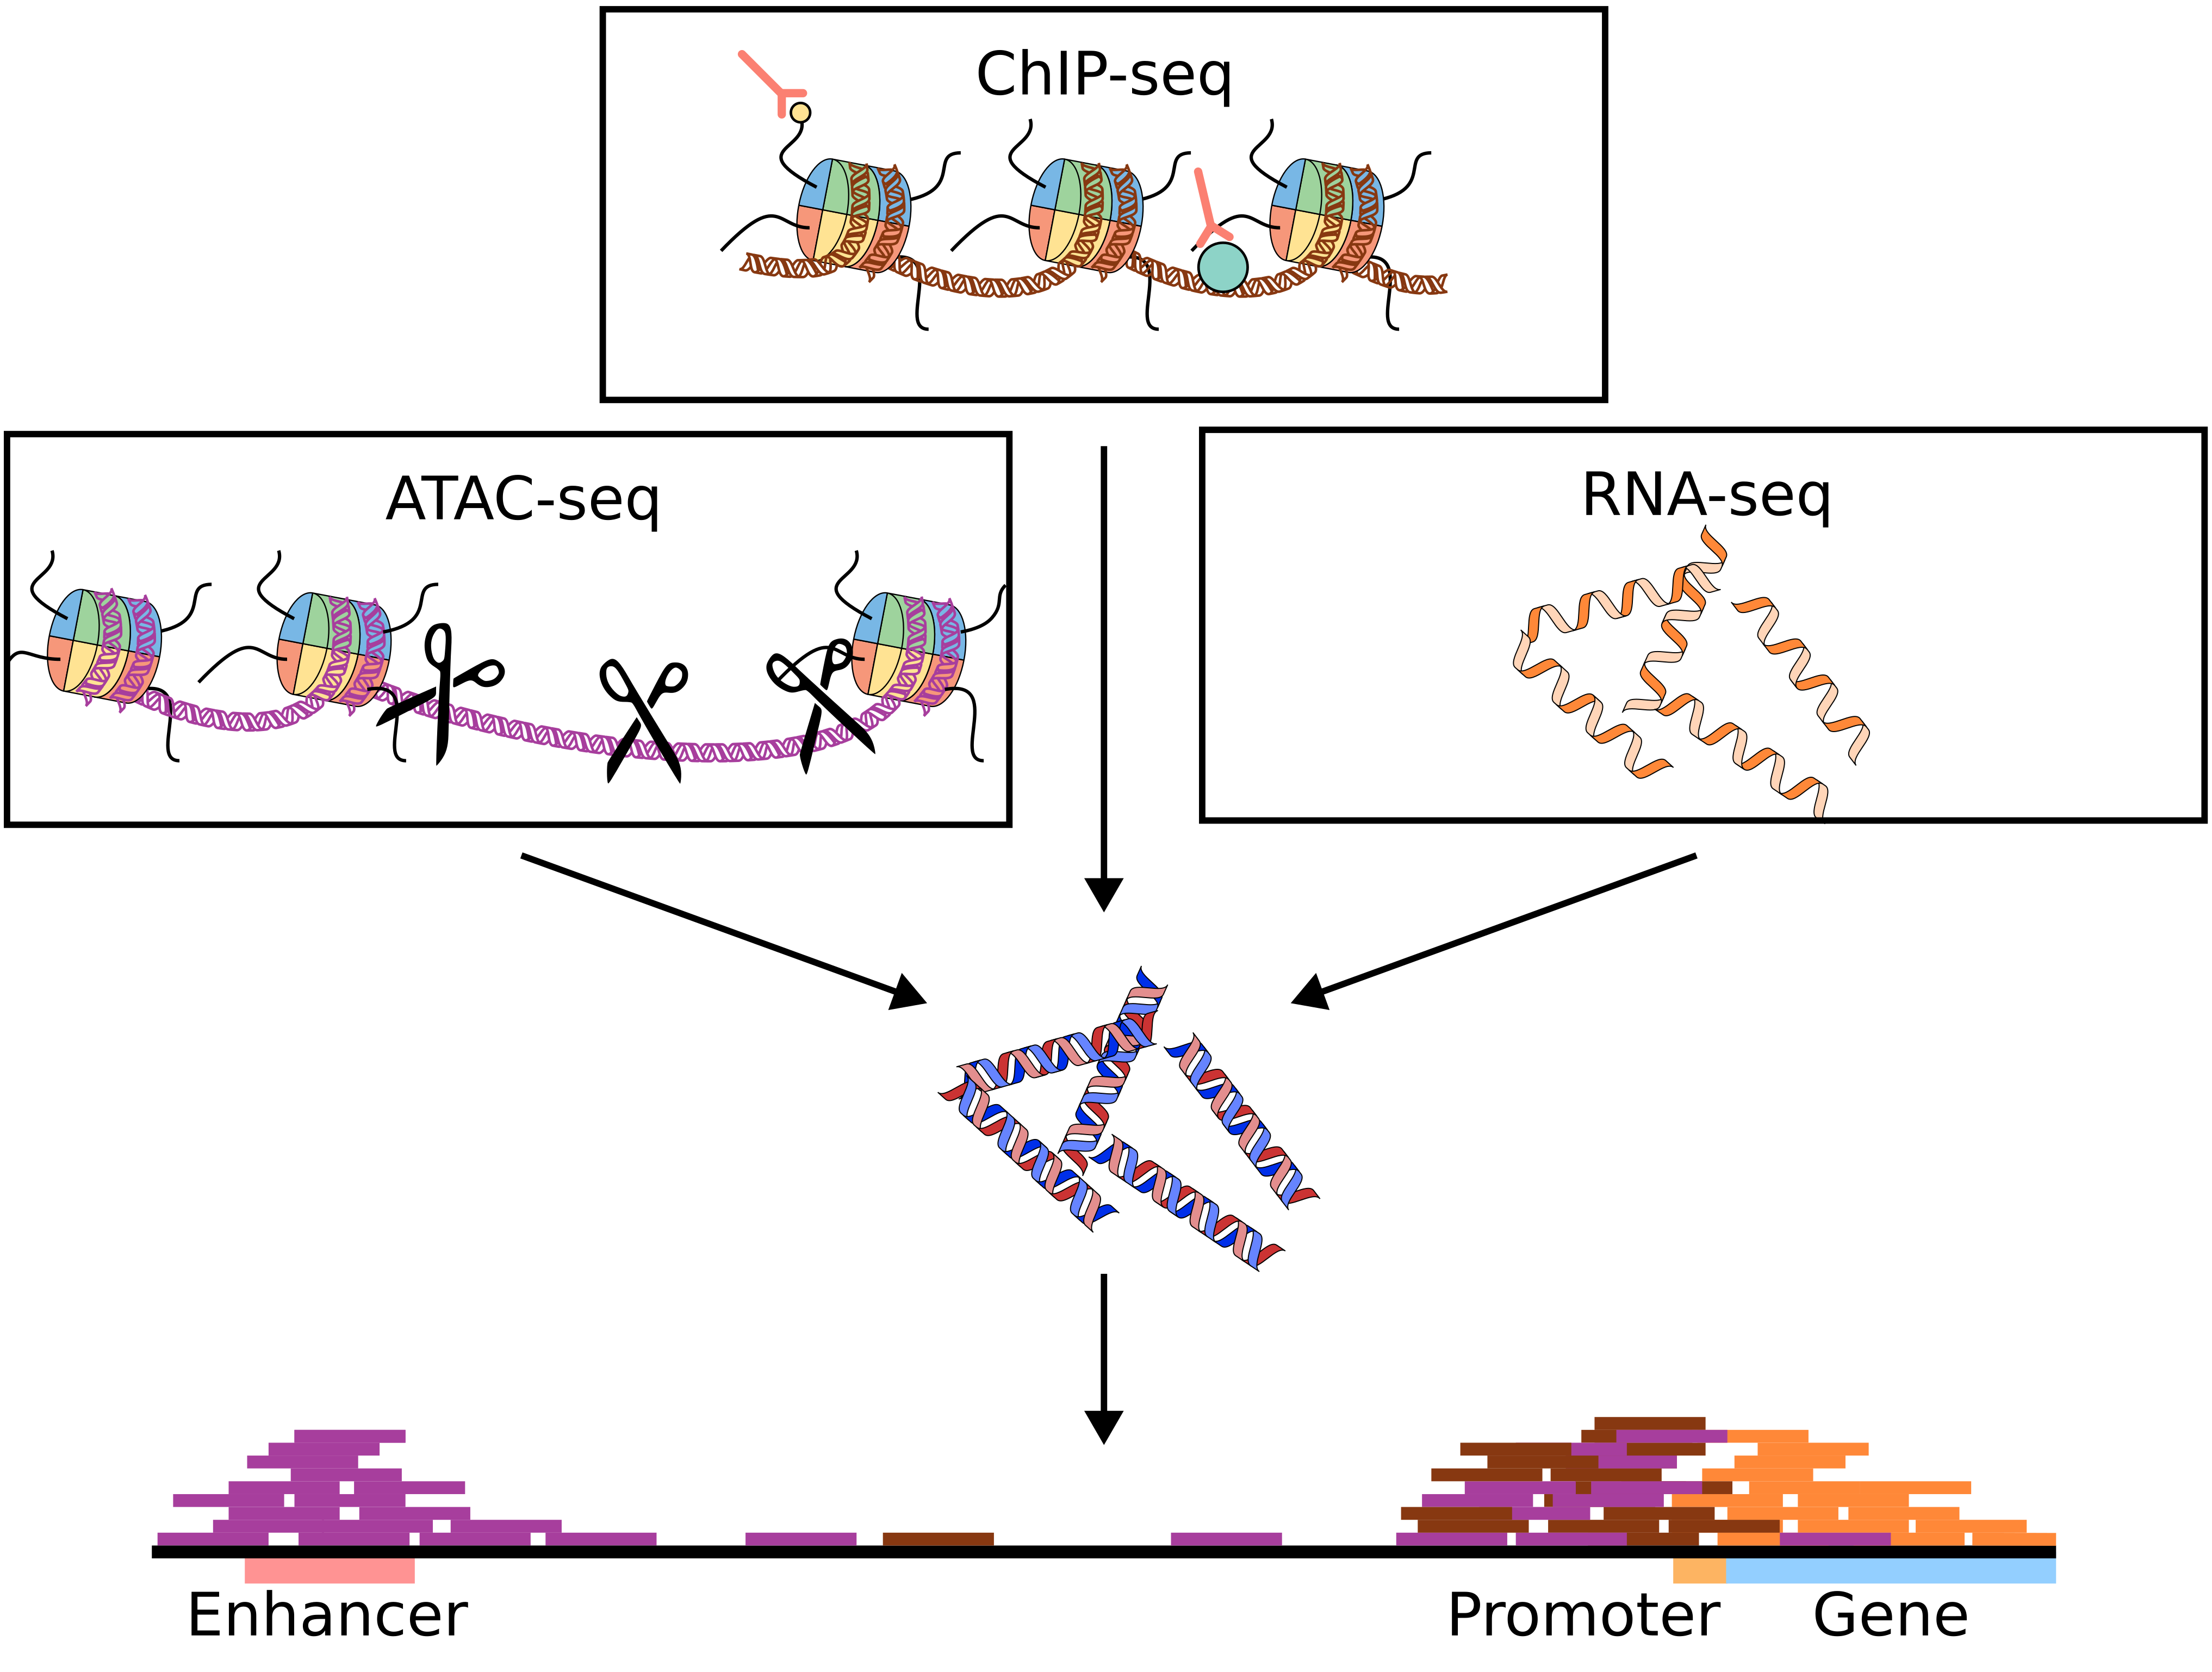
\includegraphics[width=\linewidth]{ch1.Introduction/imgs/analysis.png}
    \caption{TODO add DNAse}
    \label{fig:analysis}
\end{figure}

\subsection{Single cell}

Whereas originally 

\section{Thesis overview}

The expression and regulation of (embryonic) development is a widely studied topic. It is less common, but still common, to study gene regulation in the context of evolution. Wh

In \textbf{chapter 2} we review the current computational approaches to model and understand gene regulatory networks. Moreover, we highlight three recent developments for gene regulatory network inference which improve the power of these methods.

In \textbf{chapter 3} we discuss the implementation of seq2science, a next-generation pre-processing workflow. Seq2science supports

In \textbf{chapter 4} we discuss the molecular basis of the phylotypic stage and its related models...

In \textbf{chapter 5} 

In \textbf{chapter 6} 



\chapter{Computational approaches to understand transcription regulation in development}
% \chaptermark{Understanding transcription regulation in development}
\chapterauthor{Maarten van der Sande*, Siebren Fr{\"o}lich*, Simon J. van Heeringen}
\section{Abstract}

Gene regulatory networks (GRNs) serve as useful abstractions to understand transcriptional dynamics in developmental systems. Computational prediction of GRNs has been successfully applied to genome-wide gene expression measurements with the advent of microarrays and RNA-sequencing. However, these inferred networks are inaccurate and mostly based on correlative rather than causative interactions. In this review, we highlight three approaches that significantly impact GRN inference: (1) moving from one genome-wide functional modality, gene expression, to multi-omics, (2) single cell sequencing, to measure cell type-specific signals and predict context-specific GRNs, and (3) neural networks as flexible models. Together, these experimental and computational developments have the potential to significantly impact the quality of inferred GRNs. Ultimately, accurately modeling the regulatory interactions between transcription factors and their target genes will be essential to understand the role of transcription factors in driving developmental gene expression programs and to derive testable hypotheses for validation.

\section{Introduction}

Multicellular organisms develop from a single fertilized egg, guided by the genetic information encoded in the genome. Cell lineages diverge and form tissues and organs, based on the interplay between signaling pathways, biomechanical forces \cite{Mammoto_2012} and the regulation of gene expression programs \cite{Cameron_1987}. While development is controlled on many levels, transcription regulation is crucial \cite{TODO3}. To better understand these regulatory principles in development and evolution, it is essential to construct informative models of gene regulation.

Transcription is regulated by transcription factors (TFs) within the chromatin context \cite{Li_2004}. TFs bind the DNA either directly, mostly in a sequence-specific manner \cite{McMahon_1984}, or indirectly via other TFs \cite{Gord_n_2009}. They can recruit various other proteins, such as co-activators, RNA polymerase, chromatin remodelers and histone modifying enzymes, to remodel or stabilize the chromatin or to activate or repress transcription \cite{Chen_2021,Vaquerizas_2009}. In metazoans, TFs form up to 8\% of the known proteome \cite{Lambert_2018,Seb_Pedr_s_2018}, with DNA binding domains and affinities being highly conserved between metazoans \cite{Nitta_2015,Schmidt_2010,Villar_2014}. They bind specific DNA motifs that are clustered in relatively short cis-regulatory elements (CREs) that can be categorized as promoters, enhancers and insulators \cite{Levine_2005}. The exact function of an element depends on the combination of bound transcription factors, which is influenced by motif specificity, distance between motifs and motif directionality \cite{Avsec_2021,Brown_2007,Farley_2016,Wong_2020,Zeitlinger_2020}. Core regulatory modules and pathways involved in germ layer and axis formation are deeply conserved in metazoans \cite{Martindale_2005}.

A useful abstraction to study transcription regulation is a network of transcription factors and their target genes. This concept of a gene regulatory network (GRN) was introduced in 1969 by Roy Britten and Eric Davidson and later experimentally demonstrated in sea urchin embryos \cite{Britten_1969,Davidson_2002}. GRNs serve to predict the effect of transcription factor expression on gene transcription and to derive testable hypotheses for validation. More generally, they function to model cell type specification and differentiation in development as well as regulatory perturbations in disease. GRNs have been constructed, mostly based on experimental loss-of-function and gain-of-function studies, for a variety of developmental models. Examples include germ layer formation in echinoderms \cite{Cary_2020,Peter_2011,Saudemont_2010} and frogs \cite{Charney_2017,Koide_2005,Rankin_2011,Sinner_2006}, neural crest formation \cite{Lukoseviciute_2018,Williams_2019}, the Drosophila gap gene network \cite{Jaeger_2010} and hematopoietic development \cite{Kueh_2011,Pimanda_2010,Singh_2014}. However, experimental elucidation of a limited number of interactions is hard to scale. Regulatory interactions are highly context-specific \cite{Farley_2016,Ryan_2019} and most remain unknown \cite{Vaquerizas_2009,2012}.

Computational inference of genome-wide GRNs was made possible with the advent of expression microarrays. Expression levels between transcription factors and their target genes tend to correlate \cite{Ideker_2001} and genes with similar mRNA expression patterns are more likely to be regulated by a common transcription factor \cite{Allocco_2004,Eisen_1998}. This led to the conception of gene co-expression networks, where functional connections between genes are inferred by expression pattern similarity. WGCNA \cite{Zhang_2005} and ARACNe \cite{Margolin_2006} were among the first gene co-expression-based tools and remain popular. Presently, a multitude of GRN inference methods exists. Reviews on the technical details can be found here \cite{Levine_2005,Chasman_2017,Delgado_2019,Mercatelli_2020}. Recent advances in experimental and computational techniques means that GRN inference has progressed beyond simple co-expression. In this review, we will highlight three approaches that have the potential to significantly impact GRN modeling: (1) moving from one modality, gene expression, to multi-omics, (2) single cell sequencing for cell type-specific signal and (3) neural networks as flexible gene regulatory models (Figure \ref{fig:compapproach}).

\begin{figure}[H]
	\centering
	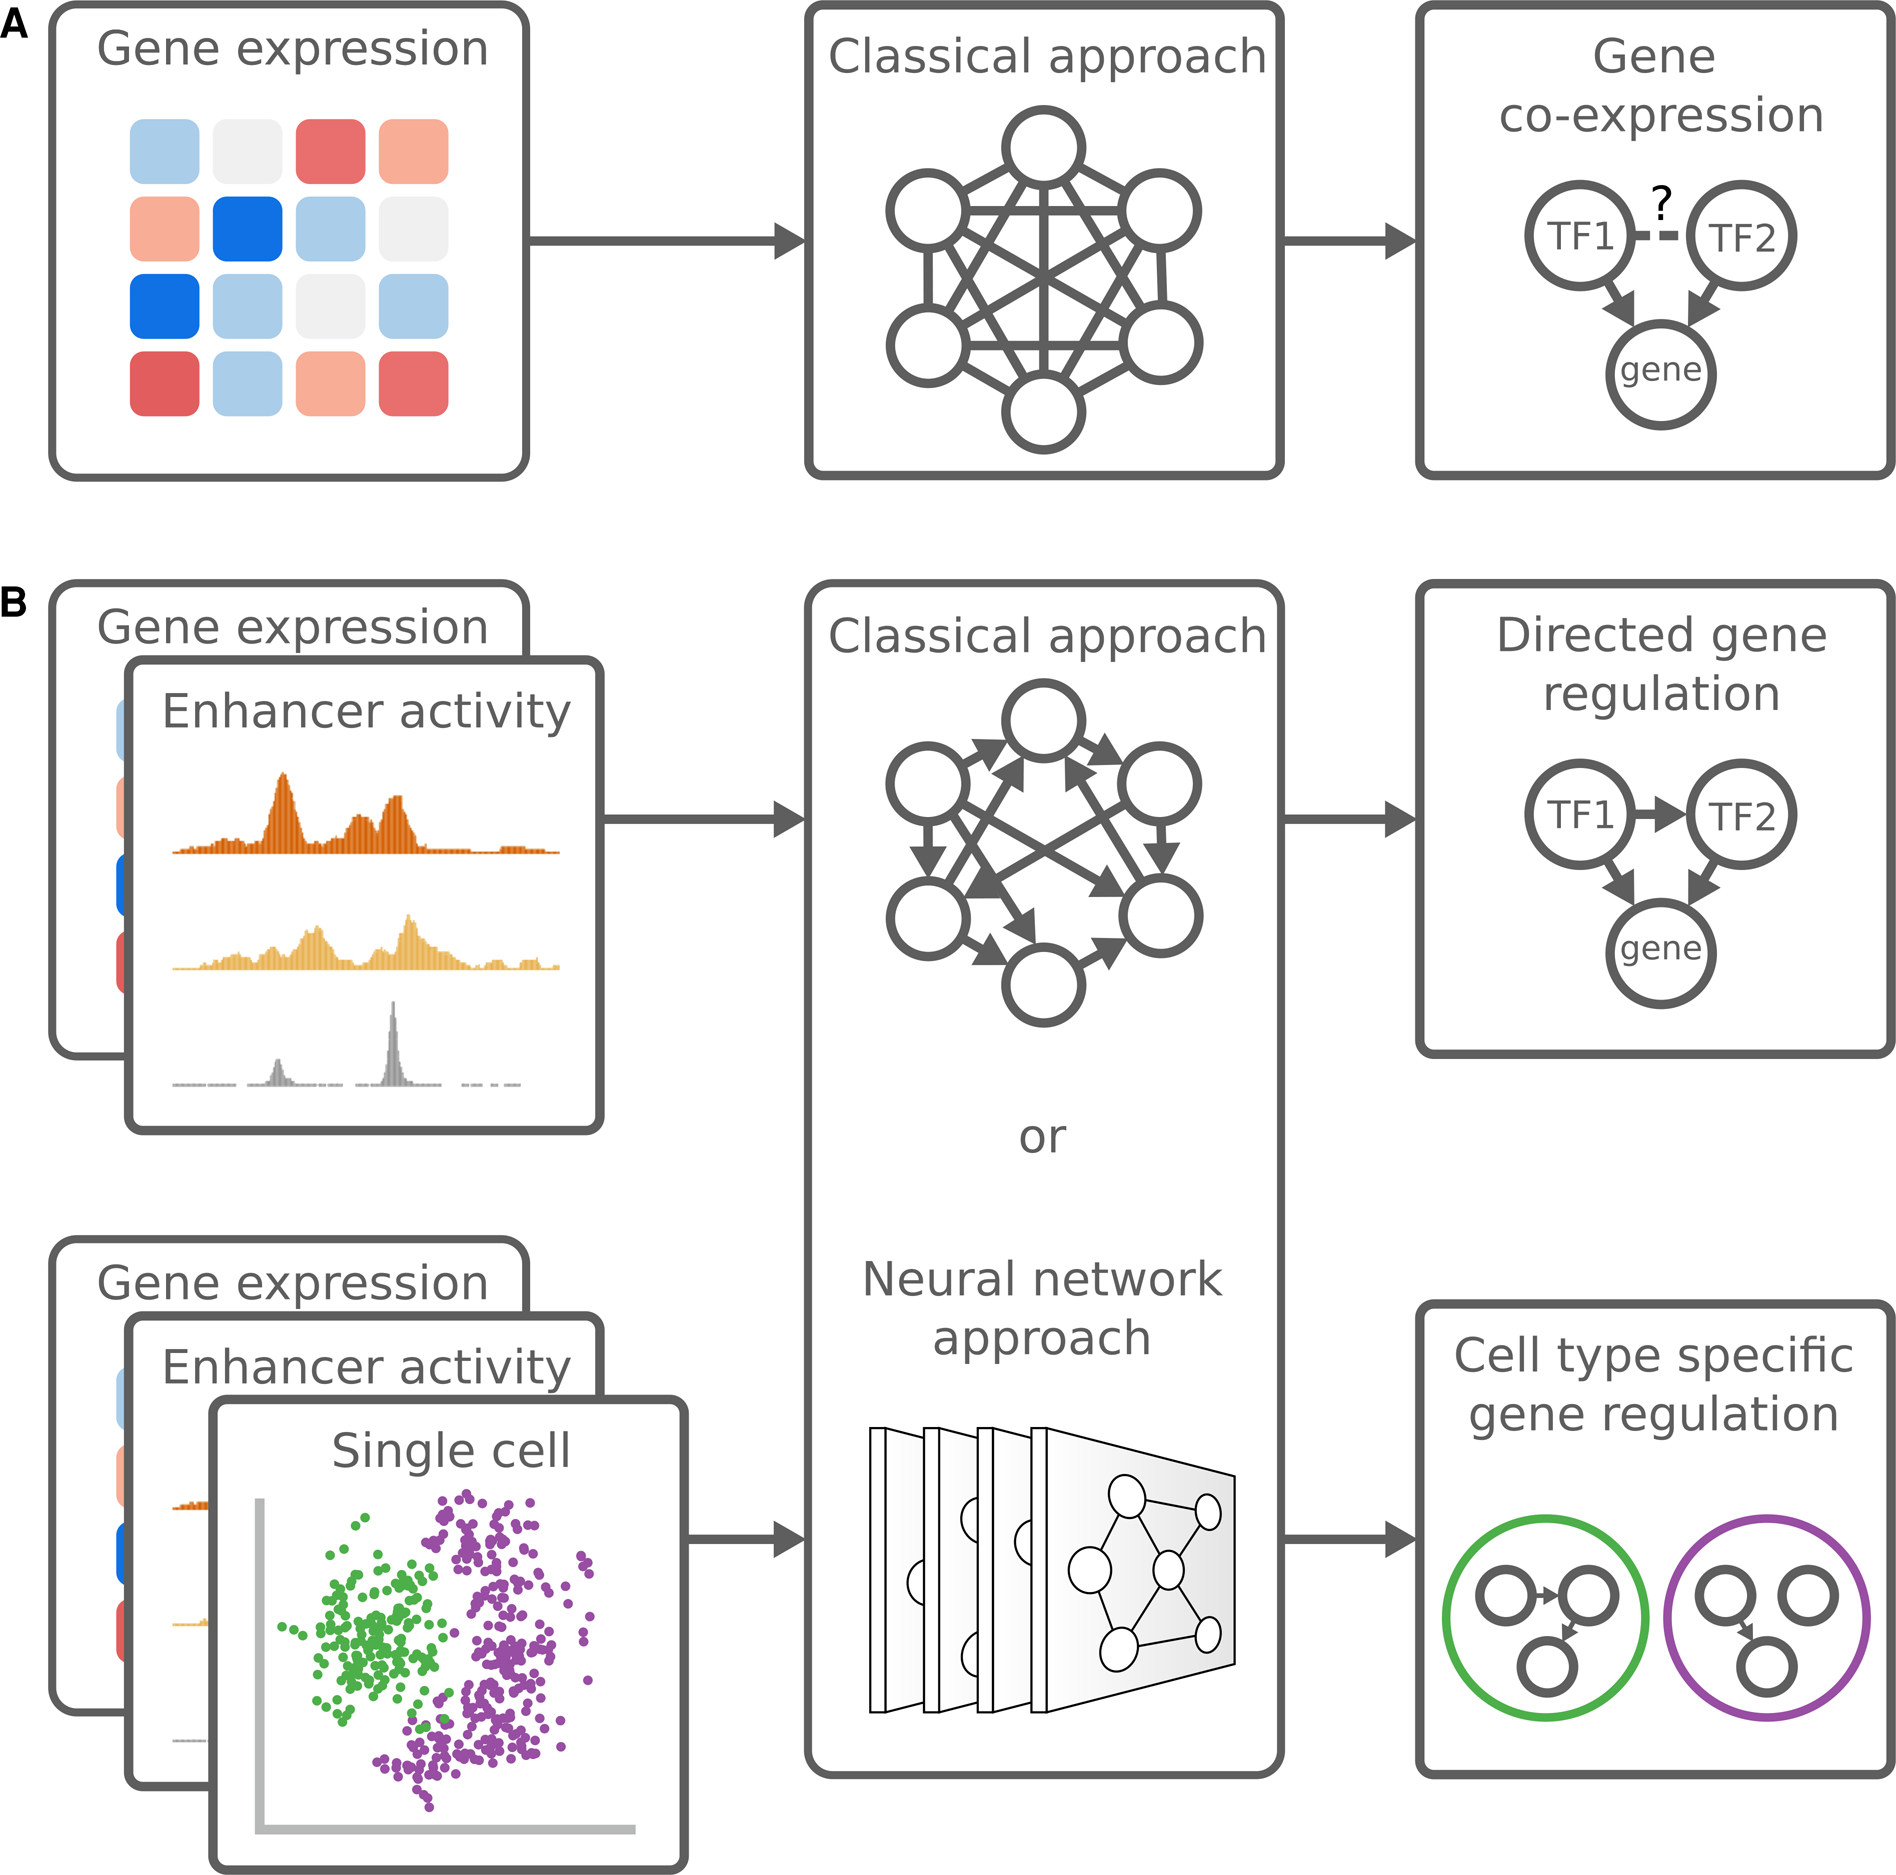
\includegraphics[width=0.8\textwidth]{ch2.compapproach/images/compapproach(1).png}
	\caption{\label{fig:compapproach}\textbf{Schematic overview of different gene regulatory network inference approaches.} \textbf{(A)} Classical approaches, e.g. correlation, regression or mutual information, can be applied on gene expression data to generate undirected co-expression networks. With prior knowledge about TFs the directionality between TF and target gene can be inferred, however, the directionality between two TFs cannot be established. \textbf{(B)} More recent approaches combine multiple types of genome-wide functional data (multi-omics), with either a classical approach or neural networks to identify directed gene regulatory networks. Single cell sequencing allows for the identification of cell type specific regulatory networks.}
\end{figure}

\section{Multi-omics to capture gene regulation}

Gene regulation by TFs is mediated through CREs including promoters and enhancers. By incorporating TF binding at enhancers, regulatory networks can be constrained by direct, causal relationships. Ideally, binding of TFs would be determined experimentally with chromatin immunoprecipitation followed by sequencing (ChIP-seq) \cite{Robertson_2007} or related techniques \cite{He_2015,Rhee_2011,Kaya_Okur_2019}. While large compendia of TF binding profiles in different cell types have been collected for humans \cite{2012}, this effort remains unfeasible for less well-studied organisms, including most developmental model systems. With sufficient training data, TF binding can be computationally imputed \cite{Keilwagen_2019,Li_2018,Quang_2019,Chen_2021,Mariani_2020,Li_2021,Bruse_2018,Schreiber_2020,TODO58,Behjati_Ardakani_2019,https://doi.org/10.48550/arxiv.2112.07571,Yi_2022,Pap_2021,Karimzadeh_2022,Koo_2020,https://doi.org/10.7303/syn6131484}, however, this does not necessarily generalize across species \cite{Cochran_2022}. As a result, most current approaches use relatively simple models that combine experimentally measured CRE activity with TF binding motifs to computationally predict TF binding.

Putative CREs and their activity can be mapped genome-wide using chromatin accessibility assays, such as DNase I hypersensitive sites sequencing (DNAse-seq) \cite{Boyle_2008} and Assay for Transposase-Accessible Chromatin using sequencing (ATAC-seq) \cite{Buenrostro_2013}. The number of reads in an element can then be used as a measure for CRE activity in the experimental system \cite{Buenrostro_2015}. ATAC-seq especially has been widely applied in developmental model systems, as it is experimentally relatively straightforward \cite{Williams_2019,Seb_Pedr_s_2018,marletaz2018,Uesaka_2019,P_lfy_2020,Shashikant_2018,Madgwick_2019,Esmaeili_2020,Bright_2021,Yang_2020}. The chromatin environment can supply additional information on CRE location, function and activity. For instance, the transcriptional co-activator p300 is a histone acetyltransferase and can acytelate lysine 27 of histone H3 (H3K27ac). ChIP-seq using antibodies specific to p300 or H3K27ac can therefore identify active enhancers and promoters \cite{Visel_2009,Creyghton_2010}. Other histone modifications that can be linked to CRE activity include H3K4me1 (enhancers) and H3K4me3 (promoters) \cite{Heintzman_2007}.

CRE activity is determined by (in)direct binding of several TFs \cite{Simeone_1988,Mitchell_1989}. Therefore, characterizing TF binding at enhancers can identify their relative importance to the function of an enhancer. One approach to infer TF binding from genome-wide DNA accessibility is digital genomic footprinting \cite{Hesselberth_2009}, which has been used to directly infer GRNs \cite{Neph_2012,Neph_2012}. However, sequence bias of the enzymes needs to be taken into account and TFs with more dynamic binding kinetics, such as some nuclear receptors, are not detected by footprint analysis \cite{He_2013,Sung_2016,Sung_2014}. Regardless, footprint analysis using cleavage bias correction can still be informative, especially in differential conditions \cite{Li_2019,Bentsen_2020}. A more routinely applied approach is to combine TF binding probabilities derived from TF motif scores with DNA accessibility. In some approaches, these are used as priors or constraints on network topology, where the network is inferred from gene expression measurements \cite{Miraldi_2019,Siahpirani_2016,Sonawane_2021}. In alternative approaches, TF motif scores and accessibility are combined with RNA expression using regression models or co-variation of accessibility and expression \cite{Madsen_2017,Kamal_2021,Schmidt_2018,Xu_2020,Ghaffari_2021,Vijayabaskar_2019}.

Enhancers regulate transcription via context-dependent enhancer-promoter interactions \cite{Levine_2010}, usually within a transcriptionally active domain \cite{Nora_2012}. Combined with TF binding data, these interactions allow for the inference of directed GRNs. Enhancer-promoter interactions can be identified experimentally with Chromatin Conformation Capture techniques \cite{Dekker_2002,Lieberman_Aiden_2009,Mifsud_2015}, although this is still uncommon in non-model systems. Inferring interaction between enhancers to target genes is an active field of research. The most commonly used heuristic is to link enhancers to the nearest gene. However, this heuristic is often still incorrect \cite{Sanyal_2012,Li_2012}. Accuracy can be improved by combining enhancer to gene distance with TF-target gene co-expression \cite{Marbach_2016}. Finally, Activity-by-Contact based models significantly outperform the nearest gene heuristic by using enhancer to gene distance and enhancer activity \cite{Fulco_2019}.

By combining gene expression data with at least one source of enhancer data (e.g. accessibility or interaction data), directed regulatory networks may be inferred with significantly higher accuracy compared with traditional co-expression approaches \cite{Xu_2020,Mercatelli_2020,Glass_2013}. Not only does the combined approach filter out spurious interactions and add causality, but it also reduces the biases introduced by singular approaches. Therefore, we believe that the use of multiple omics will become dominant in all modalities of GRN inference approaches.

\section{Single cell sequencing for cell type specific regulation}

Developmental transcription regulation has mainly been studied by either in situ hybridization \cite{Jensen_2014}, which maps the spatial distribution of gene expression of a small set of genes, or bulk gene expression studies \cite{Wang_2009}. The latter measures the whole transcriptome as a compound signal of all the different cells present in the sample. Single cell sequencing is a fast developing technique to measure the gene expression of individual cells separately, with newer techniques even capable of tagging cells to their spatial coordinates \cite{Longo_2021,Borm_2022}. These techniques increase the number of measurements from a handful to several (tens to hundreds of) thousands. This substantial increase in data allows for interesting new ways of GRN inference, but poses new challenges as well.

The output of a single cell experiment generally consists of count tables containing several thousands of cells with low coverage, e.g. only a few thousand of measured transcripts per cell. The low coverage makes the detection of relations between lowly expressed genes difficult. Although it is possible to artificially increase the sequencing depth by simulation (imputation), this does not seem to improve GRN inference \cite{Ly_2022,McCalla_2021}. Furthermore, it is important to note that cells are repeated measures \cite{Zimmerman_2021}, meaning that the cells come from the same environmental and genetic background, which breaks most statistical assumptions. Computationally clustering related cells, called pseudobulk or meta-cells \cite{Baran_2019}, and using their combined signal solves the issues of low coverage and repeated measures, and still yields cell-type specific signals.

Since fundamentally there are small differences between bulk and pseudobulk data, it is not uncommon to apply bulk GRN inference approaches, such as gene co-expression, ARACNE \cite{Margolin_2006} and GENIE3 \cite{Huynh_Thu_2010}, to pseudobulk data without much adjustment.

The large number of cells, however, allows for specialized single cell GRN approaches. These include mutual information in combination with partial information decomposition \cite{Chan_2017}, gene coexpression \cite{Aibar_2017}, self organizing maps \cite{Jansen_2019}, or a combination of single cell RNA-seq and single cell ATAC-seq coexpression and/or bayesian ridge regression \cite{Gonz_lez_Blas_2022,Jiang_2021,Kamimoto_2020}. Other approaches first order cells by their inferred temporal ordering and then infer the gene-gene relations on this pseudotime, with the assumption that these orderings, also called trajectories, represent cell lineages \cite{Packer_2019}. Pseudotime can be estimated by simply following the first principal component, or finding the minimal spanning tree between clusters \cite{Wolf_2019}, where more advanced methods smoothen the tree \cite{Qiu_2017,Street_2018}. A downside of these techniques is that they can not infer the directionality of the relationships. To computationally obtain this directionality, the ratio between spliced and unspliced transcripts per gene can be used as a proxy for whether or not a gene is actively transcribed. By applying this logic across all genes and all cells, one can infer a vector field of velocities of cells which then can be used to get a temporal cell ordering with a start and end \cite{Bergen_2020,La_Manno_2018}. These orderings then allow for inferring ordinary differential equations \cite{Aubin_Frankowski_2020,Matsumoto_2017}, Granger causality \cite{Deshpande_2022,Papili_Gao_2017,Qiu_2020}, boolean networks \cite{Woodhouse_2018} or autoregressive models \cite{Sanchez_Castillo_2017}. Most of these methods assume Gaussian noise for gene expression, even though transcription occurs in bursts \cite{Chubb_2006,Larsson_2019}, a phenomenon that can only be captured on a single cell level. These dynamics can be modeled as a Markov process including transcriptional bursting and degradation \cite{Ventre_2022}. Theoretically these mechanistic models could be great tools for hypothesis generation, but more work is needed to prove their practical usefulness. Even though the aforementioned GRN inference methods were developed for single cell data specifically, many fail to show consistent improvement over methods that were developed for bulk data, and are seemingly barely any better than purely random models \cite{McCalla_2021,Chen_2018,Pratapa_2020}. Moreover, the added complexity and number of cells leads to computational scaling issues, with some methods taking several days to weeks to finish \cite{McCalla_2021}.

Single cell sequencing has the advantage that it disentangles the composite signal present in all biological tissues. The increased number of measurements allows for more complex GRN definitions and inference. Finally, it allows for the inference of fine grained temporal orderings necessary for GRN inference. Even though single cell GRN inference methods have not yet brought the improvements over bulk methods we hoped for, we still expect single cell GRN inference to become the new standard of the field.

\section{Neural networks as flexible gene regulatory models}

Computational inference of a GRN depends on a lot of implicit assumptions. For example, a common assumption is that the relationship between genes is additive, which means that the effect on a gene equals the sum of the effects of two regulators separately, but in reality, gene-gene relationships are more complex and for example can include multiplicative effects \cite{Kim_2021}. A type of model that requires little explicit specification about the possible relationships in the data, but automatically learns these relationships, is an Artificial Neural Network (ANN). ANNs have been successfully applied in a variety of settings, with famously complex problems such as protein folding \cite{Jumper_2021}, image recognition \cite{TODO147}, and the board game Go \cite{Silver_2016}. The successes of ANNs in these unrelated fields shows great promise for application in the field of gene regulatory inference.

Just like GRNs, ANNs consist of nodes and edges. Each edge multiplies the signal from the previous node to the next, and by applying a function to the sum of all the incoming edges the value in the next node is calculated. By adding multiple layers of nodes in between the in- and output nodes (this is where the term deep neural network comes from), a network is formed that is capable of learning more and more complex interactions. Learning happens by giving the model examples of input data and expected output, and based on this information the model iteratively updates (learns) its edge weights. After training, hypotheses can easily be tested by systematically querying the model for the predicted effect of certain changes. See \cite{Eraslan_2019} for an excellent review on the topic applied to genomics.

ANNs in genomics were first applied to predict the output of a genomic assay, for instance histone modifications in a certain cell type, by using only the DNA sequence as input. Early models showed that convolutional neural networks are capable of predicting functional effects of noncoding variants from short (10–1000 bp) genomic sequences alone \cite{Alipanahi_2015,Zhou_2015}. These types of models can be used to discover composite motifs and periodic binding \cite{Avsec_2021}. Additionally, these models are capable of learning complex and distal biological relations, as increasing the input sequence to 131 kb still improves accuracy \cite{Kelley_2018}.

Whereas ANNs in genomics have mainly been popularized on sequence data, adoption for GRN inference has been relatively slow. Different approaches consist of self-organizing maps \cite{Jansen_2019}, variational autoencoders \cite{Shu_2021}, extreme learning machines \cite{Rubiolo_2017}, or graph convolutional neural networks \cite{https://doi.org/10.48550/arxiv.1806.06975,Wang_2020}. Even though these networks differ in architectural designs, they all report higher levels of accuracy over non-ANN approaches. However, without independent benchmark studies it is hard to verify these results.

The main strength of ANNs is that they can approximate any continuous relationship in the data \cite{Cybenko_1989,Hornik_1989}, with the downside that large amounts of training data are required. This makes the combination of single cell sequencing and ANNs promising, as current single cell GRN inference approaches have scaling issues \cite{McCalla_2021} and ANNs train relatively fast with the use of GPUs (specialized graphics cards). Fundamentally, understanding how ANNs work is, however, much harder than understanding the classical models typically used for GRN inference. This causes ANNs to be met with skepticism and the persistent misconception that ANNs only function as a black box for predictions and its logic can not be interpreted \cite{Zhang_2021}. We expect ANNs to become commonplace in the field of GRN inference due to their successes in other fields, ease of implementation with high-level programming libraries \cite{TODO160,https://doi.org/10.48550/arxiv.1912.01703}, and availability of sufficient training data due to single cell sequencing.

\section{Discussion}

Traditional GRNs, mostly based on gene co-expression, have so far served as a useful abstraction to understand regulatory dynamics in developmental systems. However, the way GRNs are currently derived suffers from two fundamental problems. First, the classic GRN that describes TF to target gene relations remains a simplified model and, by design, cannot properly reflect the full complexity of gene regulation. In addition, they are mostly based on mRNA expression as a measure of protein expression, even though this relation is not always linear \cite{de_Sousa_Abreu_2009}. In addition, any other types of regulation between transcript and protein product, such as mRNA degradation and post-translational modification, are usually ignored. Second, experiments generally have more features (i.e. genes measured) than samples which is also known as ‘the curse of dimensionality'. In this underdetermined system, many different models can potentially fit to the data, and it is both practically and theoretically impossible to identify the correct model with certainty \cite{Krishnan_2007}. It then should not come as a surprise that benchmarks consistently demonstrate that the quality of the inferred GRNs is low \cite{Chen_2018,Pratapa_2020,Cokelaer_2016,TODO165,Guo_2017,Marbach_2012,STOLOVITZKY_2007}. Based on these observations it is clear that our current approach to infer GRN is not sustainable and design changes are needed. Ultimately, we expect the field to move towards GRNs inferred from neural networks trained on single cell multi-omics data.

Having said that, it is not enough to just naively apply single cell multi-omics ANNs. By adding more modalities, and making GRNs more complex, networks become even more underdetermined. This is why most multi-omics approaches use the new modalities to prune the possible TF-target gene relations, which actually reduces the degrees of freedom \cite{Xu_2020,Aibar_2017,Jiang_2021,Kamimoto_2020}. Moreover, one can use time-series data to further prune TF-target gene interactions \cite{Zoppoli_2010}, although time-series multi-omics GRN inference tools are still relatively uncommon \cite{Ernst_2007,Schulz_2012,Ding_2018,Conard_2021}. In addition, computational methods such as regularization \cite{TODO174} and dropout \cite{TODO175} constrain the problem in such a way that you end up with the simplest fit out of likely possible fits. In addition, recent developments have made it possible to measure multiple modalities in the same cell, such as combined ATAC-seq and RNA-seq \cite{Ma_2020,Cao_2018,Chen_2019}, which offers new, exciting opportunities for combining single cell sequencing with multi-omics data. ANNs, finally, have been made relatively easy to implement, can learn any type of interaction, and make no assumptions about the data (such as normality), which makes them extremely powerful GRN tools. However, it is not yet clear what the optimal architecture is for these networks, and interpreting the learned network from the ANN remains difficult.

GRN inference has become a data science, and it is time that we start treating it as such. Integrating multiple omics, several thousands of cells, and training complex machine learning models requires specialized knowledge. Common mistakes, such as treating cells from the same sample as independent \cite{Zimmerman_2021}, double dipping \cite{https://doi.org/10.48550/arxiv.2012.02936}, and data leakage \cite{Schreiber_2020}, can be avoided by proper data science training, but are unfortunately still common. Comparing the quality of GRN inference methods requires standardized benchmarks with multiple datasets, preferably a mix of experimental data and simulated data \cite{Dibaeinia_2020,Li_2022,Ventre_2022}. Simulated data has the advantage that the ground truth is known which makes benchmarking straightforward, but has the clear disadvantage that the quality of simulated data depends on its assumptions and may actually not be representative of real biological data. The DREAM challenges \cite{Cokelaer_2016,TODO184} and BEELINE platform \cite{Pratapa_2020} are great examples, with predefined datasets and quality metrics. Only by measuring network accuracy in equal settings will it be possible to properly compare methods. It is however important to note that the goal of GRN inference is to gain mechanistic insights, as opposed to getting an optimal benchmark score, which makes fair comparison between approaches hard.

All together, we expect the field of transcription regulation in development to move towards increasingly multimodal GRN inference techniques to identify causal relations between genes. Single cell sequencing adds a cell type-specific precision which bulk sequencing can not provide. Finally, we expect the adoption of artificial neural networks as the field matures in technology and formal training, as these methods are inherently more powerful as previously used techniques.

\section{Perspectives}

\begin{itemize}
    \item Gene regulatory networks have served as powerful models to understand gene regulatory programs in development and disease. Amongst others, these networks have been applied to model developmental patterning, to identify relevant transcription factors for cell fate transitions and to characterize deregulated transcriptional programs in disease.
    \item We believe three relatively recent developments will impact the computational inference of GRNs. The combination of multiple data modalities, such as RNA expression and DNA accessibility, help to constrain GRN topology and to predict directed networks. Single cell sequencing will become the de facto standard, as it allows for cell type-specific models and is able to provide the high number of measurements that are needed. Finally, artificial neural networks have the capability to create flexible and powerful models of gene regulation, which will benefit efficient and accurate GRN inference.
    \item The developments outlined above have the potential to significantly improve GRN inference. To fully exploit these approaches we have to implement common data science practices, and develop community-driven benchmarks to consistently measure the performance of different techniques.
\end{itemize}

\section{Competing Interests}

The authors declare that there are no competing interests associated with the manuscript.

\section{Funding}

Netherlands Organization for Scientific Research [NWO grant 016.Vidi.189.081 to S.J.v.H.].

\section{Author Contributions}

\textbf{Maarten van der Sande}: writing — original draft and writing — review and editing. \textbf{Siebren Fr{\"o}lich}: writing — original draft and writing — review and editing. \textbf{Simon J. van Heeringen}: writing — review and editing, funding acquisition, and supervision.


\chapter{Seq2science}
\chapterauthor{Maarten van der Sande*, Siebren Fr{\"o}lich*, Tilman Sch{\"a}fers, Jos Smits, Rebecca R. Snabel, Simon J. van Heeringen}

\chapter{Crucial controls missing in comparative studies with regards to the phylotypic stage}
% \chaptermark{The phylotypic stage}
\chapterauthor{Maarten van der Sande, Marlien Kolmus, Gert Jan C. Veenstra, Simon J. van Heeringen}
\section{Abstract}

The phylotypic stage, characterized by the highest degree of similarity during embryonic development between species of the same phylum, has gained support through molecular evidence. This study re-evaluates three previous molecular studies on the phylotypic stage and uncovers issues with their experimental design. We propose three crucial controls to identify these problems in future studies. Additionally, we advocate for a re-definition of the phylotypic stage, as it is ambiguous in its current form.

\section{Introduction}

Embryonic development is a complex and highly orchestrated process that begins with a single fertilized egg and culminates in the formation of a multicellular organism with a defined body plan and specialized organs. Even though morphologically the egg and the adult can be vastly different between two related species, there is often a period of remarkable similarity in early development. This period of similarity is known as the phylotypic stage, and over the years many different theories and explanations for its existence, or whether it even exists or not, have been proposed\cite{Kalinka2012,Irie2014,Drost2017}. 

The idea of a morphologically similar embryonic stage dates back to Aristotle\cite{Aristotle1943}, but were formalized and popularized by Karl Ernst von Baer and Ernst Haeckel. In the early 1800s von Baer formulated his four laws of embryology. His first law states that \textit{the more general characters of a large group appear earlier in the embryo than the more special characters}. This means that as an embryo develops, it first develops its oldest phylum-specific features, to then respectively develop its class, order, family and species-specific features. Haeckel instead formulated the recapitulation theory, popularized by the phrase \textit{ontogeny recapitulates phylogeny}. The recapitulation theory states that an embryo consecutively develops from embryonic stages of lower species to stages of higher species. In its strongest form, the recapitulation theory has been discredited, as development is not a repetition of evolution. Nonetheless, Haeckel's observations of similarities between embryos of different vertebrate classes, have, together with von Baers’ laws, formed the basis for the current models of evolutionary development

This has led to two competing models of evolutionary development, the hourglass model and the funnel model (also known as the early-conservation model). The hourglass model is based on the model proposed in 1954 by Paul Medawar\cite{Medawar1954}. Medawar argues that somewhere mid-embryogenesis is the most morphologically conserved stage for vertebrates. This has since been generalized across phyla and even kingdoms (plants\cite{Quint2012} and fungi\cite{Cheng2015}), where each phylum now has their own stage of maximum similarity during mid-embryogenesis. The funnel model, based on von Baers' laws, instead predicts the highest morphological similarity early in development. The phylotypic stage, initially called the \textit{phyletic stage}, refers to the point of maximum similarity in these models\cite{Cohen1963, Seidel1960}. More recently an inverse hourglass model has been proposed, where specifically the beginning and end of embryonic development seem conserved between species of different phyla, and the least molecular similarity is seen at the phylotypic stage\cite{Levin2016}.

Whereas the phylotypic stage has originally been defined based purely on morphological descriptions alone, the definition is gradually being extended to contain quantitative and molecular features. For example the idea that HOX genes are the master regulator of the phylotypic stage for vertebrate development\cite{Duboule1994}. Even more recent there have been genome-wide comparisons of genes and regulatory elements. These quantitative comparisons can roughly be divided into two distinct approaches; (i) calculating a conservation metric for a single time series for each time point, where conservation metrics include for instance the average evolutionary age of transcripts\cite{DomazetLoso2010}, gene mutation rate index\cite{Quint2012, Piasecka2013}, embryonic lethality\cite{Uchida2018}, relation between timing of DNA accessibility and its evolutionary age\cite{Uesaka2019}, and variance between replicates\cite{Liu2020, Uchida2022}. These results are usually visualized as a figure where one axis represents embryonic development, and the other the calculated conservation metric. The second approach (ii) compares orthologous features between time points of two time-series directly. Orthologous features that have been compared are cell type proportions\cite{Mayshar2023}, gene expression similarity\cite{Irie2011, Kalinka2010, Levin2016, marletaz2018}, and regulatory DNA accessibility similarity\cite{Hu2017, Liu2021}. The comparison between two time-series is usually visualized as a heat map, where the axes represent embryonic development per species, and the color represents (dis)similarity. Both of these quantitative approaches have been used to study the phylotypic stage, but there are subtle differences in the conclusions one can draw depending on which method is used. 

While quantitative studies are seen as offering an unbiased approach to studying the phylotypic stage, the results can be heavily influenced by experimental design, which highlights the importance of incorporating appropriate controls. To give some examples; based on morphological timings both an hourglass\cite{Cordero2020} and a within-phylum inverse hourglass\cite{OlafRP2003} have been found. Based on RNA-seq data Chan \textit{et al.} found an hourglass pattern, but with the same analysis on microarray data they find no temporal conservation pattern\cite{Chan2021}. Piasecka \textit{et al.} find that the observed conservational pattern is highly dependent on the metric used, for instance TODO that the protein sequence of regulatory regions is most conserved for genes expressed in mid-development, gene duplication and new gene introduction is most constrained during early development, but all gene properties coherently show the least conservation for the latest stages\cite{Piasecka2013}. Moreover, a popular similarity metric, the transcriptomic age index\cite{DomazetLoso2010}, expresses completely different conservational patterns based on whether or not the data has been log transformed\cite{Piasecka2013}. Finally, Levin \textit{et al.} found an inverse hourglass between members of different phyla\cite{Levin2016}, but in an independent re-analysis this pattern was found not to be significantly enriched\cite{Dunn2018}. 

We propose three crucial controls to address the the problem of the dependence on experimental design when studying the phylotypic stage; (i) a within-phylum comparison, (ii) a between-phylum comparison and (iii) a within-species comparison. No study about the phylotypic stage to date incorporates all three controls, and we show that by applying these comparisons on earlier analyses we find problematic statistical artefacts which lead to incorrect conclusions about the phylotypic stage. Moreover, by specifically addressing these controls the field can work towards a unified definition of the phylotypic stage and its related models.

\section{What does the phylotypic stage actually predict?}

The phylotypic stage lacks a single accepted explicit definition, but the differing definitions can roughly be divided into three main ideas; the presence of a dynamic pattern, gene regulatory complexity at the phylotypic stage, or the presence of certain key morphological characteristics\cite{OlafRP2003}. The dynamic pattern based definition describes the pattern of similarity, where similarity can both be morphological or molecular\cite{Slack1993,Duboule1994}. The pattern-based definition predicts the highest similarity at the phylotypic stage. The gene-regulatory based definition predicts that gene regulation during the phylotypic stage is so complex that small changes in gene expression result in large (deadly) effects \cite{raff1996}. Finally, the key morphological characteristics based definition specifies the presence of certain key characteristics as the phylotypic stage, for instance for vertebrates the development of the notochord, neural tube, pharyngeal arches, and somites\cite{Kimmel1995}. These different definitions are not mutually exclusive, and are often used interchangeably, but in most recent analyses the dynamic pattern based definition is the definition implicitly adhered to, simply because it is the easiest to measure.

The phylotypic stage, the hourglass model, and the funnel model do not pose explicit hypotheses on the similarities of embryos from different phyla. However, as the word phylotypic is a compound word of phylum and typical, the word is suggestive of features conserved within a phylum but not between phyla. This implies that the point of maximum similarity between phyla does not coincide with the phylotypic stages of the phyla involved. Levin \textit{et al.}\cite{Levin2016} use this implication in their inverse hourglass model as a new definition to distinguish phyla, where they note that embryonic dissimilarity is largest between species from different phyla at their respective phylotypic stages. Is it thus safe to assume that the point of maximum similarity between species from different phyla does not occur at their respective phylotypic stages? 

Similarly, what do we expect if we were to compare the embryonic development of a species against itself? The developmental models again pose no explicit expectation here. We know for instance that within-species transcriptomic variance is lowest mid-development (fig. \ref{fig:within_timepoint}), something that is used as an argument for the hourglass model\cite{Liu2020, Uchida2022}. The reasoning here is that gene regulation is most tightly regulated mid-development, and that this translates to a low transcriptomic variance between replicates. This explanation closely matches the process-based description of the phylotypic stage. But this changing variance over time will likely affect the similarity for direct comparisons between species. Is the high similarity between species at the phylotypic stage actually an effect of the higher similarity within species, or do we expect that the phylotypic stage has a higher similarity between species of the same phylum even when corrected for within-species variance?

To address these ambiguities in the description of the phylotypic stage we've re-analyzed three recent molecular studies. By specifically addressing whether the phylotypic stage exists within-species, within-phylum, and between-phyla we expose important flaws in their analyses.

\section{Re-analyses}

% The following re-analyses are all missing at least one of our proposed controls, and we show when we apply them the original conclusions get invalidated. Where possible we follow the same pre-processing and distance metrics as used in the original studies. All three of these studies apply genome-wide comparisons, where two of the studies do this based on gene expression count tables, and one based on regulatory sequence similarity.

\subsection{Amphioxus functional genomics and the origins of vertebrate gene regulation} \label{subsection:marletaz}

In the paper \textit{Amphioxus functional genomics and the origins of vertebrate gene regulation}\cite{marletaz2018} Marl\'etaz \textit{et al.} investigated the similarity of orthologous gene expression in several chordates, and consistently find a point of maximum similarity during mid-embryogenesis which corresponds to the hourglass model (\textit{Branchiostoma lanceolatum}, \textit{Danio Rerio}, \textit{Gallus gallus}, \textit{Oryzias latipes}, \textit{Xenopus tropicalis}). All comparisons are within the same chordate phylum, but comparisons between species of different phyla or within-species are missing. In our re-analysis we focus specifically on the comparison between \textit{Danio rerio} and \textit{Xenopus tropicalis} and show that the point of maximum similarity between these two species corresponds to the point of maximum similarity within each species. We show that the current analysis can not distinguish within-species effects from between-species effects.

Figure \ref{fig:betweenexperiment}B shows the pairwise similarity between all sampled stages of \textit{Danio rerio} and \textit{Xenopus tropicalis}, where similarity is based on the Jensen-Shannon distance (JSD) of the gene counts (TPMs). The JSD is a distance metric where a high value means low similarity between distributions and vice versa. The JSD follows an hourglass pattern with the point of maximum similarity at 20 hours post fertilization for \textit{Danio rerio} and at 30-32 hours post fertilization for \textit{Xenopus tropicalis}, marked by a red square. Our result is visually similar to the comparison by Marl\'etaz \textit{et al.} and the actual point of maximum similarity is adjacent to theirs, marked by a green square. The absolute JSD values are however vastly different between our and the original analysis, which is because we have opted to represent TPMs as probabilities and calculate JSD using a log base of 2. This causes the JSD to be bound between 0 and 1, which makes comparisons between different data sets easier as they are on the same scale. Figure \ref{fig:betweenexperiment}A and C show the related within-species comparisons between experiments, where we've used a similar time-series of \textit{X. tropicalis} and \textit{D. rerio} from different studies. Both these within-species comparisons show a pattern that could be interpreted as an hourglass, with a point of maximum similarity somewhere during mid-embryogenesis. Note how the points of maximum similarity within species closely match with the points of maximum similarity between species. Similarly, figure \ref{fig:withinspecies} shows all the within-species comparisons comparisons against itself, where similarly we find that there is a high self-similarity at the point of maximum similarity between species.

\begin{figure}[H]
    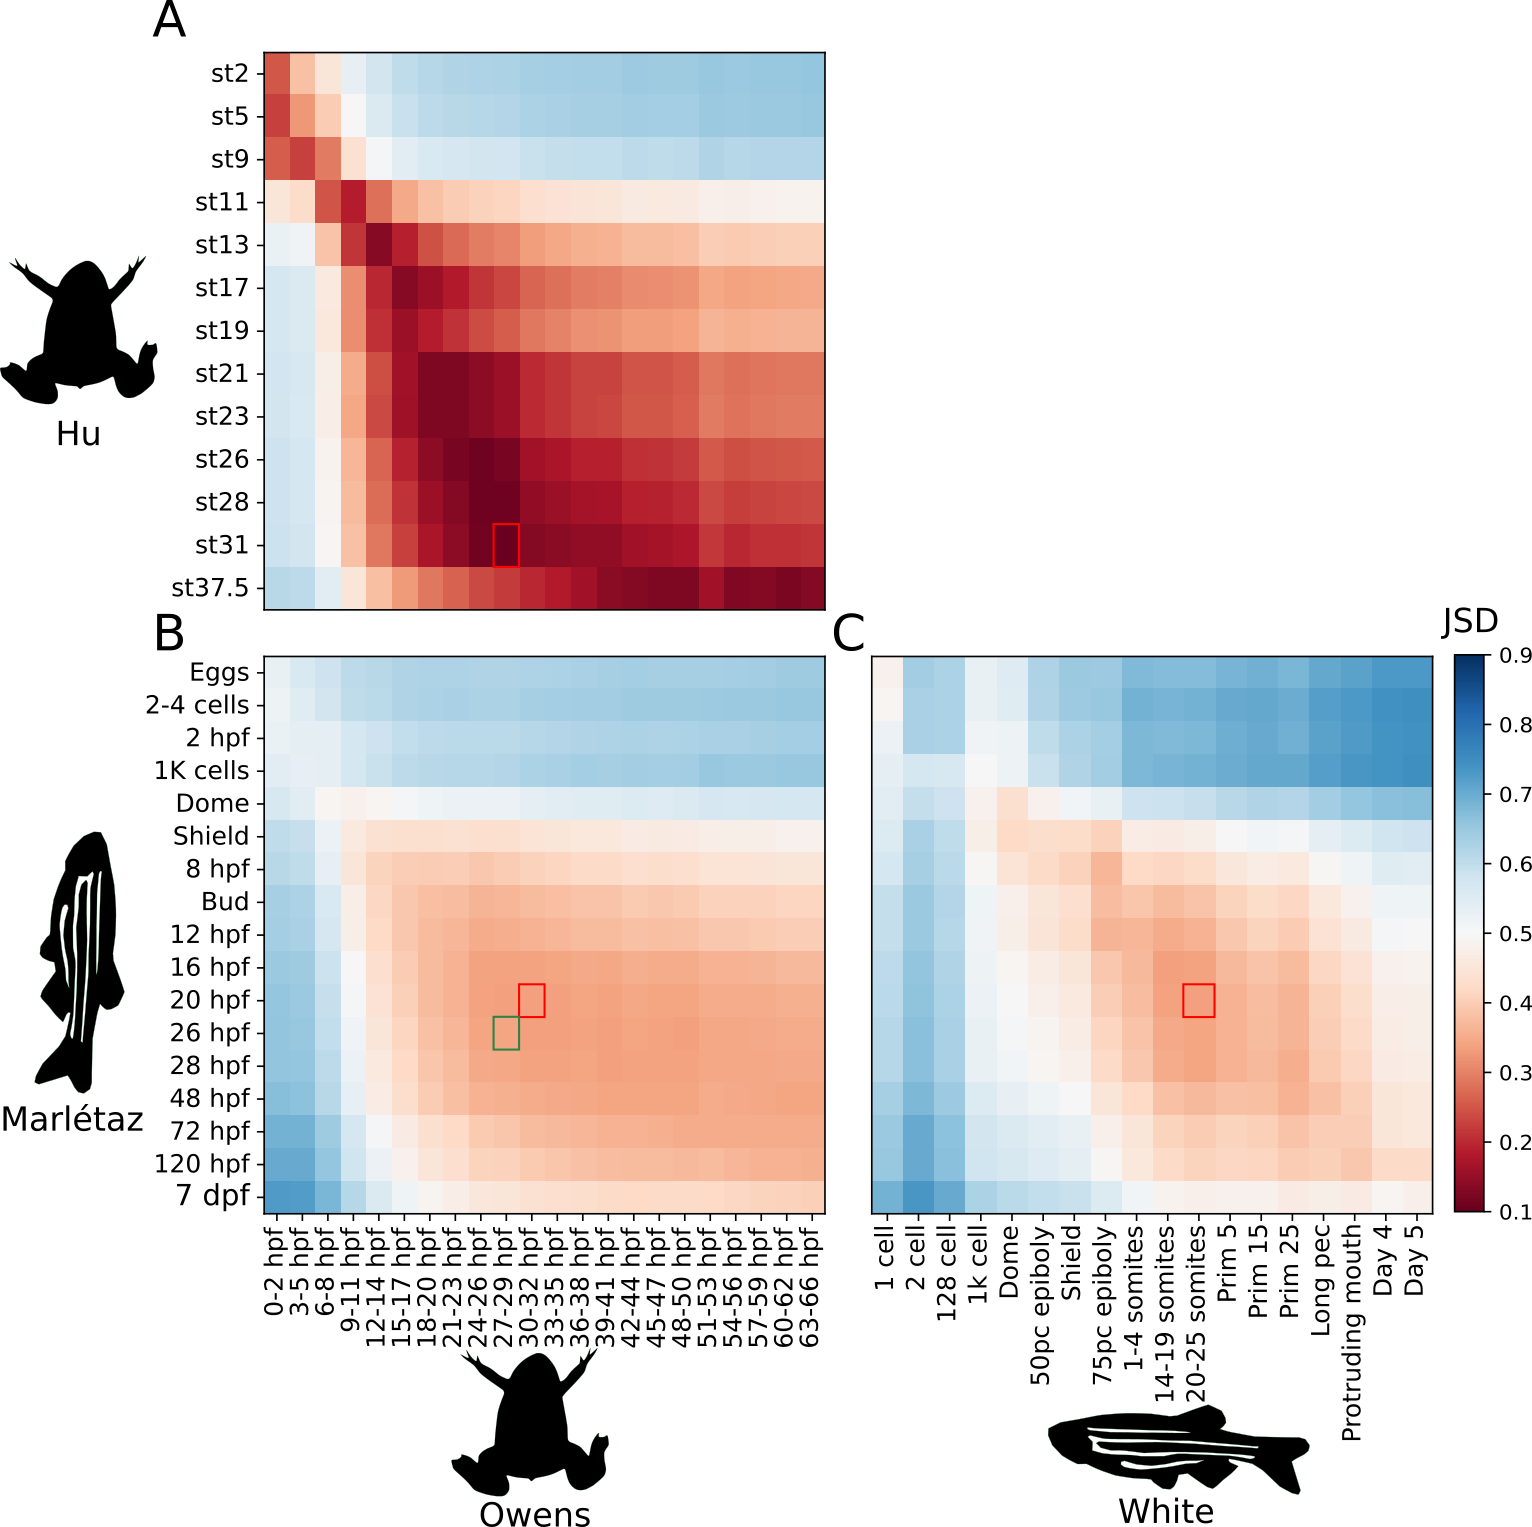
\includegraphics[width=\linewidth]{ch4.hourglass/images/between_experiment.png}
    \caption{Heatmap of pairwise Jensen-Shannon distances between (A) two \textit{Xenopus tropicalis} time series, (B) a \textit{Xenopus tropicalis} and a \textit{Danio rerio} time series, and (C) two \textit{Danio rerio} time series. The point of lowest Jensen-Shannon distance is marked in each comparison by a red square, and the green square represents the point of maximum similarity between \textit{Xenopus tropicalis} and \textit{Danio rerio} in the original study by Marl\'etaz et al.\cite{marletaz2018}.}
    \label{fig:betweenexperiment}
\end{figure}

Our re-analysis shows that an hourglass pattern already occurs in a within-species comparison. Any further comparison that is made between such time series suffers from this effect, and based on this basic re-analysis it is clear that the between-species comparison is just a superimposition of the two within-species patterns. How to correct for this effect NOT CLEAR and beyond the scope of this research, as there could be multiple explanations. The effect does not seem to be 

Still to write once finalized how we finish this:

\begin{enumerate}
    \item perhaps jensen shannon and highly expressed?
    \item not sure how to correct for it? Dividing JSD or subtracting, no clue what that means
    \item potentially works is subtracting euclidean distances, but best to leave that to real statistician + perhaps specifically generated data?
    \item we should show JSD between phyla. e.g. drosophila and c. elegans: point of max similarity happens at later time point, but time series also look quite bad.
    \item big difference zebrafish perhaps due to different sequencing protocols <-- important
    - strictly speaking between-experiment
\end{enumerate}

\subsection{The mid-developmental transition and the evolution of animal body plans} \label{subsection:levin}

In the paper \textit{The mid-developmental transition and the evolution of animal body plans} Levin \textit{et al.} compared the correlation coefficient of orthologous genes over time between ten species from different phyla. They found that most species-species comparisons had a high similarity in the beginning and a high similarity at the end of development, with a period of low similarity in the middle, which they called the \textit{mid-developmental transition}. They note that this period of low similarity between phyla seems to correspond to the phylotypic stage. They then suggest that this pattern could be used to distinguish different phyla. In this re-analysis, we demonstrate that we can find a \textit{mid-developmental transition} for both a within-phylum and between-phylum comparison. Moreover, we show that this pattern is a statistical artefact and can not be used to infer temporal conservational patterns.

Figure \ref{fig:within_phylum}A shows the pairwise Pearson correlation coefficient of one-to-one orthologs between each stage of \textit{Drosophila melanogaster} and \textit{Danio rerio}. With the same methodology of the original study we get a dual-phase pattern where both the early and the late stages between the two species seem conserved, but with a period of low conservation in the middle. If we now apply the same methodology to the chordates \textit{D. rerio} and \textit{X. tropicalis}, we get a similar biphasic pattern, indicating the \textit{mid-developmental transition} is not exclusive to between phyla comparisons. It is important to note that figure \ref{fig:within_phylum}B is based on the same count tables as figure \ref{fig:betweenexperiment}B. There are several minor differences in their processing, but the main reason for the large difference in trend is the gene standardization that is applied.

\begin{figure}[H]
    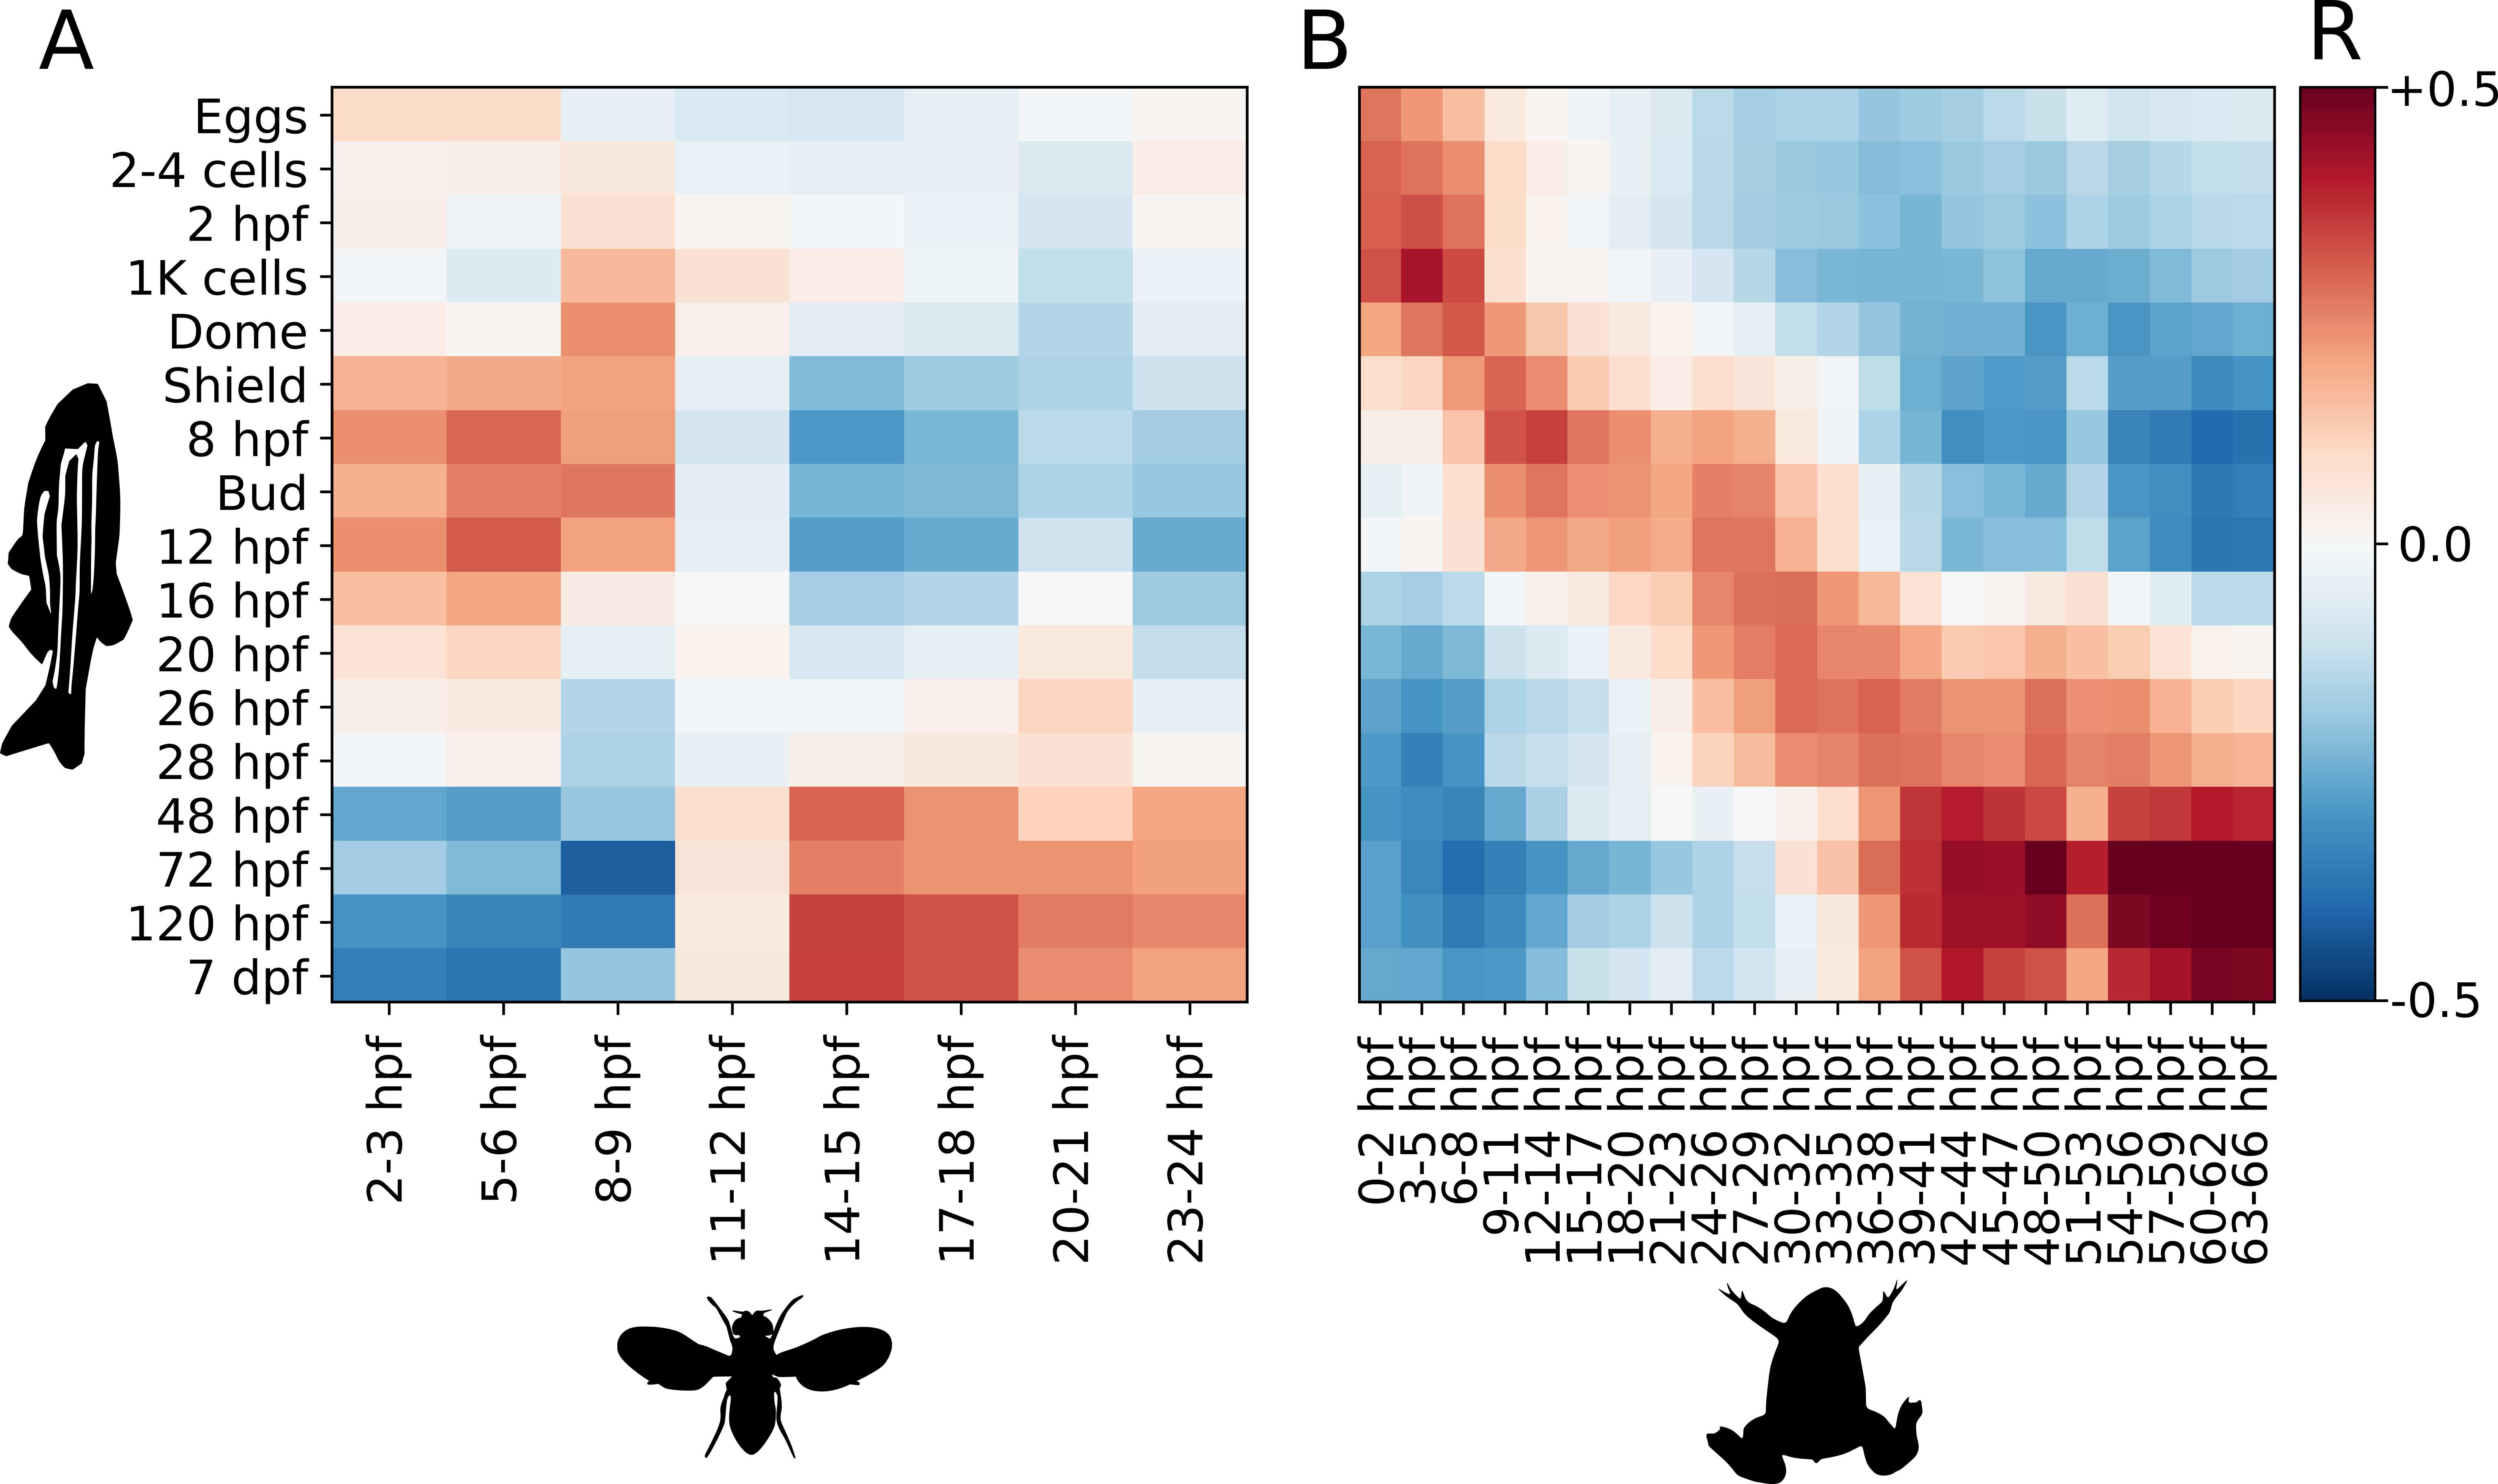
\includegraphics[width=\linewidth]{ch4.hourglass/images/within_between_phyla.png}
    \caption{Heatmap of pairwise Pearson correlation coefficients between (A) \textit{Danio rerio} and \textit{Drosophila melanogaster}, and (B) \textit{Danio rerio} and \textit{Xenopus tropicalis}. A mid-developmental transition occurs for both comparisons (between- and within-phyla).}
    \label{fig:within_phylum}
\end{figure}

Levin \textit{et al.} apply a standardization per gene. This means that each gene's counts have their mean over time subtracted and are divided by the gene's standard deviation over time. Standardization is generally a good practice for parametric methods like the Pearson correlation coefficient. In this case standardization effectively scales each gene to have equal weight in the correlation coefficient. If no standardization is applied, the extremes (the low and high expressed genes) have a higher importance in the calculation of the correlation coefficient than the rest of the genes. However, in our case standardization causes a surprising artefact. We can for instance cut each time series into halves, and after standardization, for three out of four comparisons still get a mid-developmental transition (fig. \ref{fig:normalisation}). 

\begin{figure}[H]
    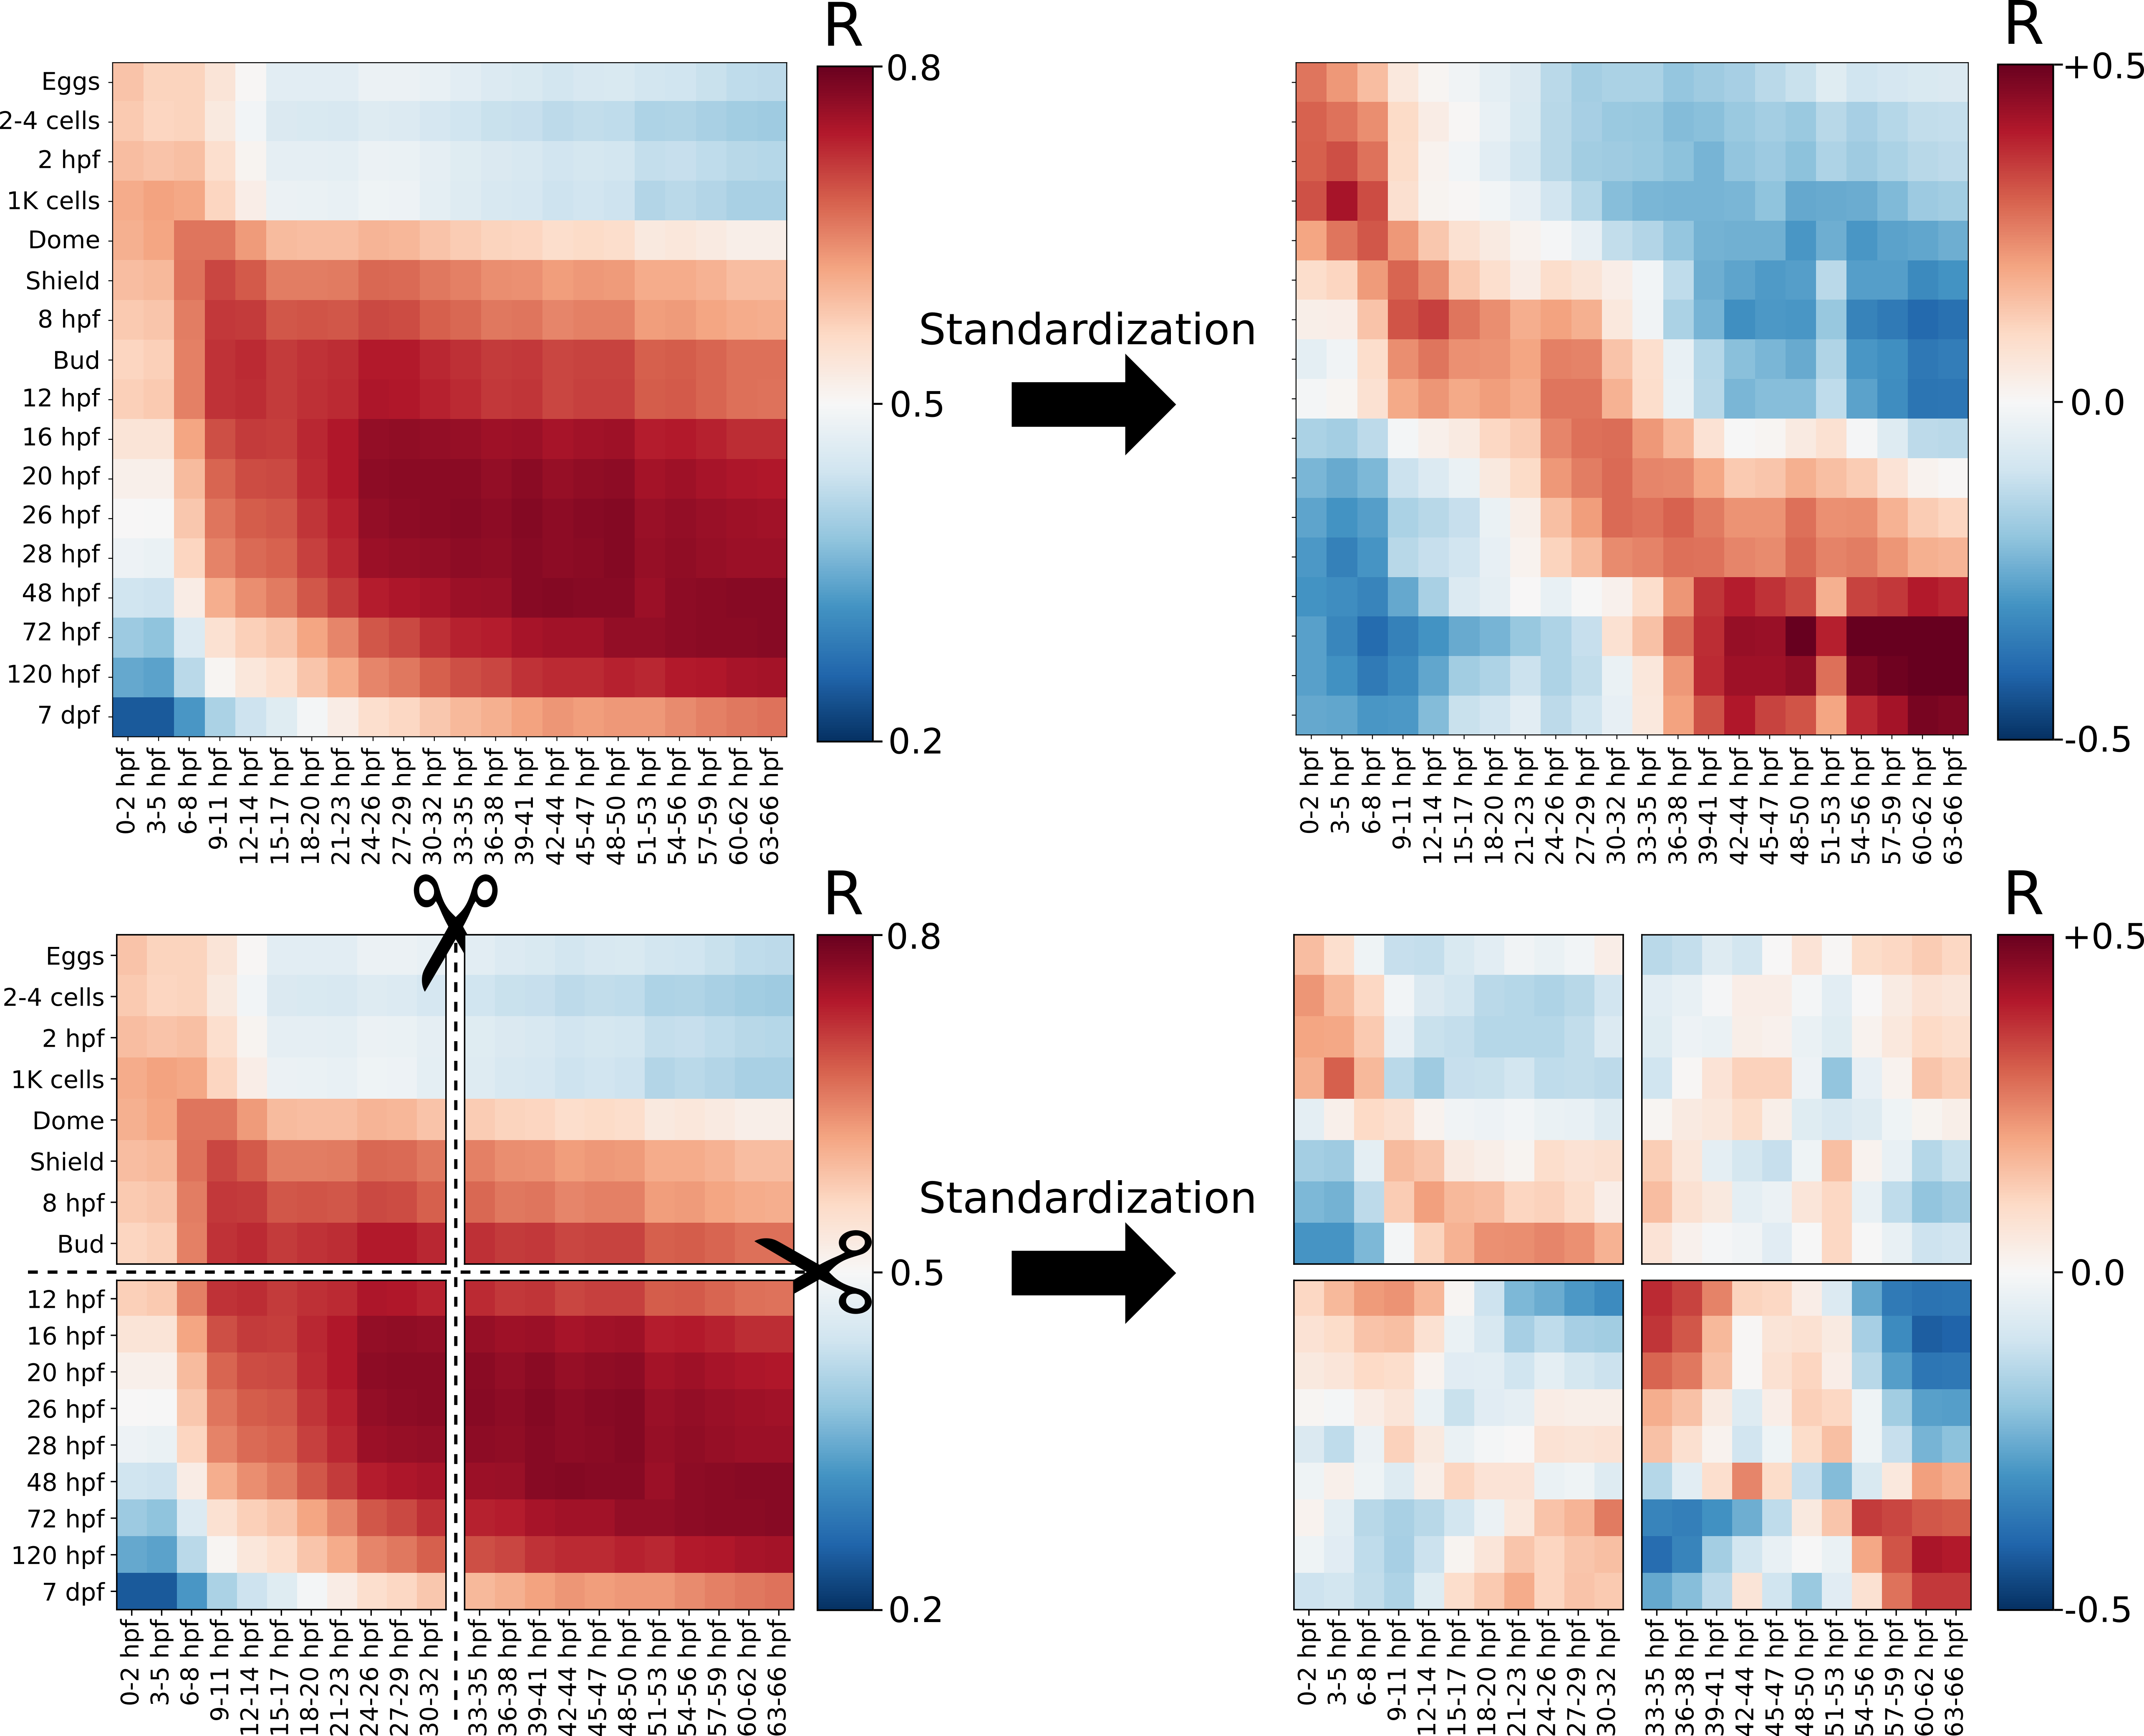
\includegraphics[width=\linewidth]{ch4.hourglass/images/normalisation.png}
    \caption{Heatmap of pairwise Pearson correlation coefficients which shows the effect of normalisation. The first image shows the not-normalised data, where each time series is cut in half. The second image shows the effect of normalisation on pairwise Pearson correlation coefficients. Whereas the original data had a point of maximum similarity approximately in the middle of the time series, three out of four subsets now show an inverse hourglass. TODO NEEDS AN A AND A B}
    \label{fig:normalisation}
\end{figure}

To get an understanding as to why this happens we need to study the patterns of gene expression during development. Similarly to Levin \textit{et al.}, we've calculated the Pearson correlation coefficient for each gene with a linearly increasing line (this is what Levin \textit{et al.} call the gene landscape in their study). A coefficient of 1 would mean that a gene is linearly going up over time, a coefficient of -1 would mean that a gene is linearly going down over time, and a coefficient of 0 would mean that a gene shows no temporal pattern. In figure \ref{fig:genelandscape} we show the histogram of Pearson correlation coefficients for \textit{D. rerio}, \textit{D. melanogaster}, and \textit{X. tropicalis} per gene over time. For each comparison we get an arc, with an enrichment for genes that are either going up or down over time, with relatively few genes having no temporal pattern. The scatterplot of Levin \textit{et al.} unfortunately hides this pattern, and a 2d histogram would have been a better choice. The explanation for as to why we get this pattern is actually pretty straightforward. Most embryos grow extensively during development, and as the embryo grows we expect the total amount of mRNA to increase as well. But, most sequencing protocols quantify a fixed amount of transcripts per sample, which means that the total of measured transcripts stays constant over time. This effectively means that genes get split into either one of two expression groups; a group where gene expression increases faster than the average gene (right side of the gene landscape), or the group where gene expression increases slower than the average gene(left side of the gene landscape). This also explains why this pattern is less pronounced for \textit{D. melanogaster}, as this embryo grows little in size during development. See figure \ref{fig:genelandscapenormalization} for the difference between per-embryo normalization and transcript per million (TPM) normalization for \textit{X. tropicalis} embryos.  

\begin{figure}[H]
    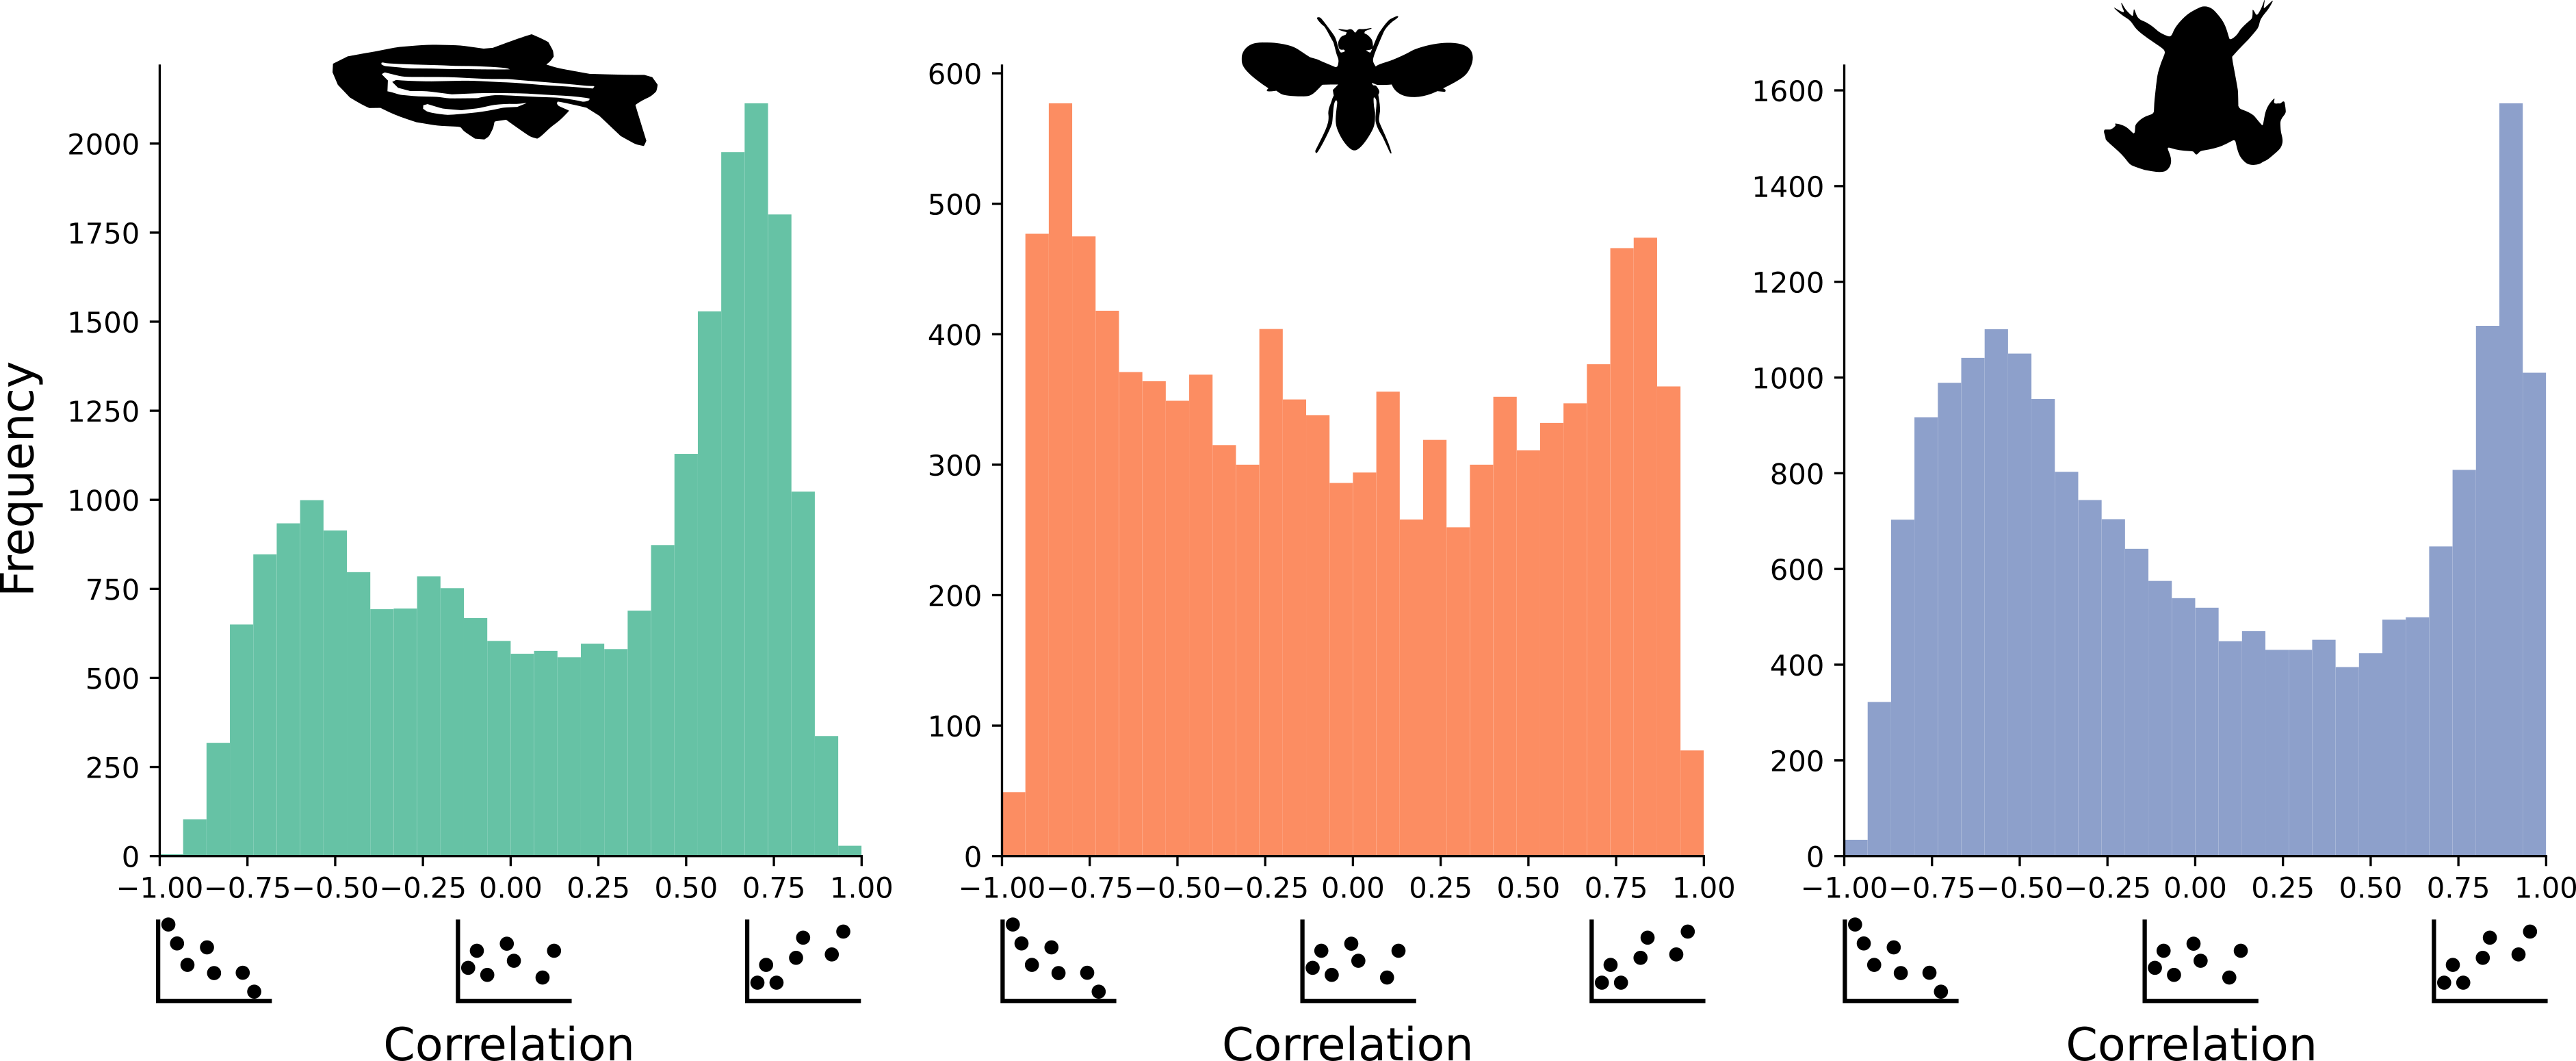
\includegraphics[width=\linewidth]{ch4.hourglass/images/gene_landscape.png}
    \caption{gene landscape TODO}
    \label{fig:genelandscape}
\end{figure}

Now that we know that our genes can be classified as either going up or going down over time, we can think about how this influences our analysis. Let's start by imagining the time-series of a single gene which has a binary expression profile, where at the start of our time-series the gene is \textit{off}, and at a random time point switches \textit{on} and stays on until the end of the series. We now imagine the expression profile of this gene in a related species, and assume again that it starts \textit{off} and at random time point switches \textit{on}. We can express the probability that these two imaginary time-series are equal (section \ref{subsection:middevelopmenttransition}), and if we visualize these probabilities it is clear these odds show a mid-developmental transition (fig. \ref{fig:inverse_math}). This theoretical derivation is a however an extreme oversimplification of what happens biologically and considers only a single gene. For this reason we simulated two time-series with a continuous expression profile. In these series half of the genes start in an \textit{off} stage where expression is zero, and half in an \textbf{on} where expression is one. Similarly as the thought experiment, these genes, at a random time-point, gradually switch from \textit{off} to \textit{on}, or vice versa (fig. \ref{fig:sim_explanation}A). We can now calculate the Pearson correlation coefficient between these simulated series, and again we get a clear mid-developmental transition. Similar to the biological data, if we cut the simulated data into halves, and apply standardization afterwards, we get a mid-developmental transition per subset of the data (fig. \ref{fig:sim_normalisation}). 

\begin{figure}[H]
    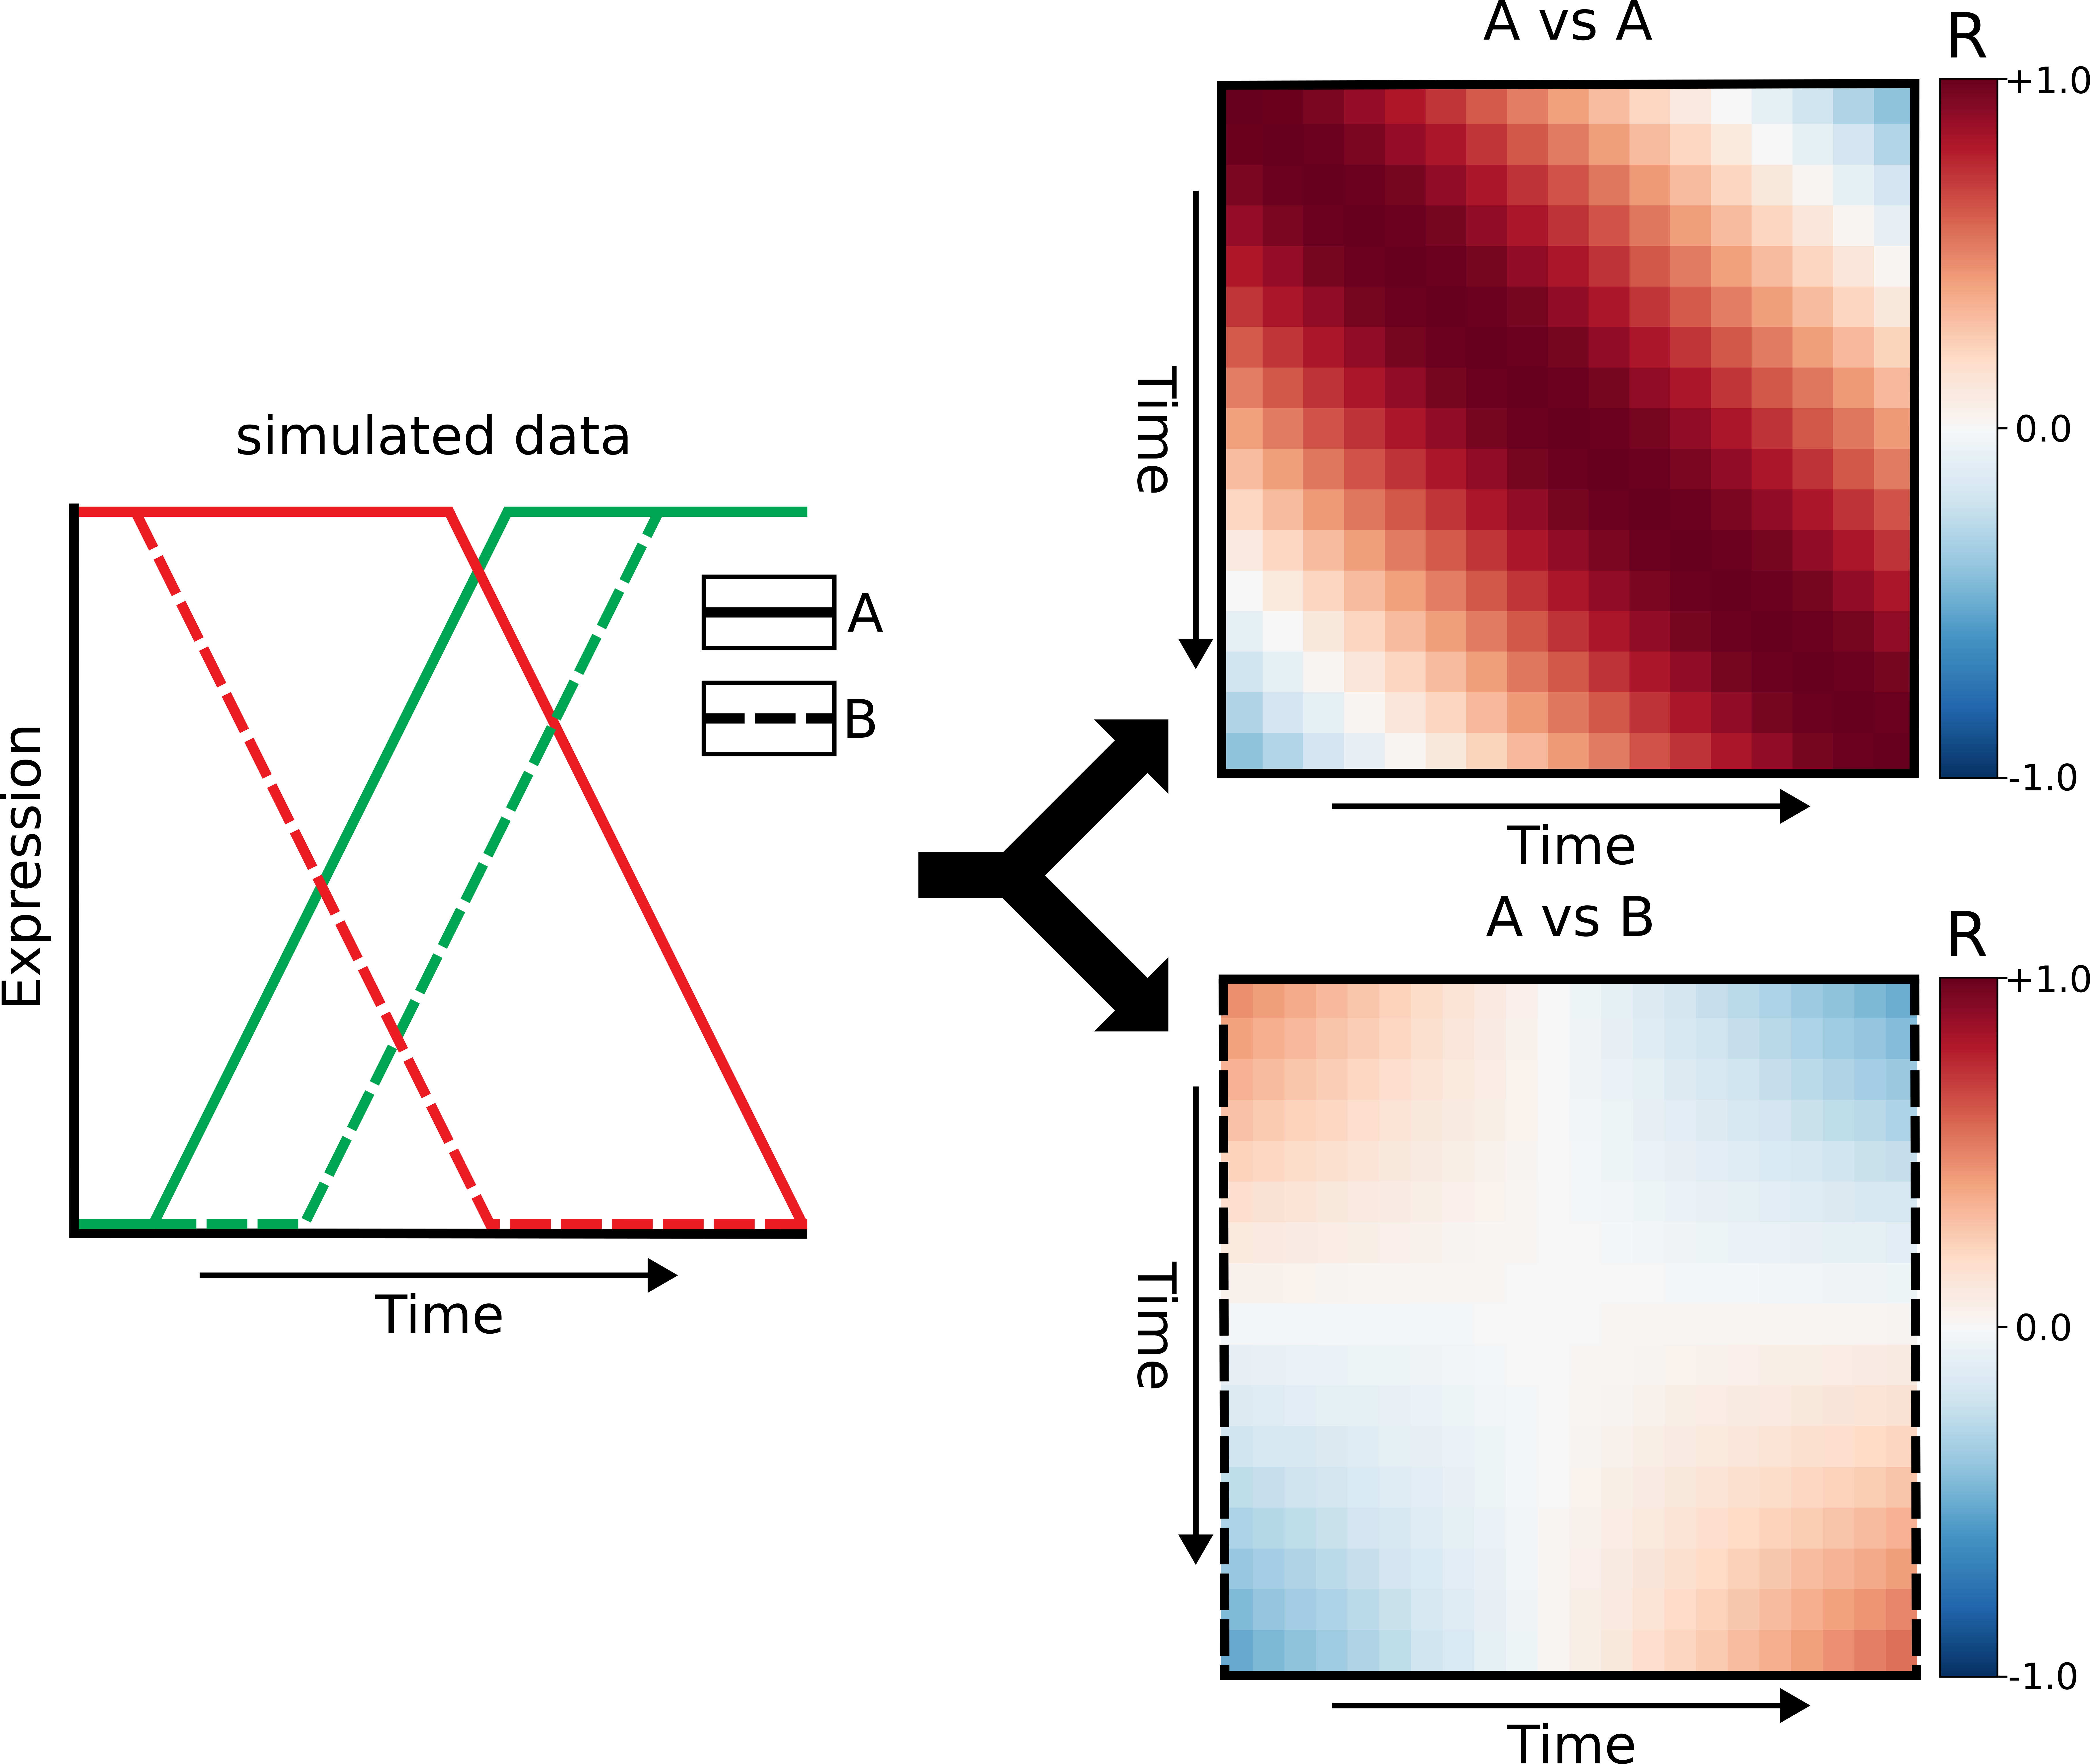
\includegraphics[width=\linewidth]{ch4.hourglass/images/sim_explanation.png}
    \caption{TODO explanation.}
    \label{fig:sim_explanation}
\end{figure}

By incorporating a within-phylum comparison it becomes clear that the mid-developmental transition is a statistical artefact of gene standardization. It can be considered a case of Simpson's paradox, where by standardization gene expression gets put into two groups (high vs low expression). Where there is no particular correlation within each group, but with a clear correlation when comparing the data set as a whole\cite{Saccenti2023}. It is important to note that we've applied the same criteria as Levin \textit{et al.} to only include dynamic genes (minimum expression of 10 and at least a log2 fold change). This means that this pattern is not caused by irrelevant and lowly expressed genes. As such we see no molecular basis for an inverse hourglass model between phyla, which leaves the question as to how the phylotypic stage behaves in comparisons between-phyla wide-open.

\subsection{The hourglass model of evolutionary conservation during embryogenesis extends to developmental enhancers with signatures of positive selection} \label{subsection:liu}

In the paper \textit{The hourglass model of evolutionary conservation during embryogenesis extends to developmental enhancers with signatures of positive selection} Liu \textit{et al.} compare the similarity of accessible regions over five matched embryonic developmental time points between two \textit{Drosophila} species (\textit{D. melanogaster} and \textit{D. virilis}). Liu \textit{et al.} find that the middle time point (TP3) uses the most enhancers, and is the most conserved between these two flies (figure \ref{fig:peak_null}B). In this re-analysis we show that this hourglass pattern can simply be explained by the different number of enhancer regions found per time point.

In this study conservation is defined as the similarity between time point specific enhancers between \textit{D. melanogaster} and \textit{D. virilis}. Time point specific enhancers are defined as enhancers that are enriched in only one time point (TP), and similarity is calculated by dividing the number of TP-specific enhancers that are enriched in both species for the same time point with the number of remaining TP-specific enhancers for that time point(Jaccard index). Figure \ref{fig:peak_null}A shows the Jaccard index per time point between \textit{D. melanogaster} and \textit{D. virilis}, with the highest value at TP3, the \textit{Drosophila} phylotypic period\cite{Liu2021}. If we apply the same methodology between replicates from \textit{D. virilis}, we get a different pattern, where TP1, TP3, and TP5 are most conserved between replicates of the same species(fig. \ref{fig:peak_null}C). This pattern between replicates indicates a potential bias in the analysis. Upon inspection it seems that the number of TP-specific enhancers seem positively correlation with the Jaccard index(fig. \ref{fig:peak_null}B,D). To test whether this relation exists we've made a consensus set of enhancers over all the time points, and assign each time point a set of randomly picked enhancers, while keeping the number of enhancers per time point the same as originally found \ref{fig:shuffle}A. This removes all biological meaning from the data, but yet, still shows the highest Jaccard index at TP3 between species. The obvious way to control for this would be to subsample all time points to the same number of peaks \ref{fig:shuffle}B. Once subsampled, we find that TP2 shows the highest conservation between enhancers between \textit{D. melanogaster} and \textit{D. virilis}. The dependence of the Jaccard index on the number of enhancers can also be formally proven, see section \ref{subsection:flypeaks}. 

\begin{figure}[H]
    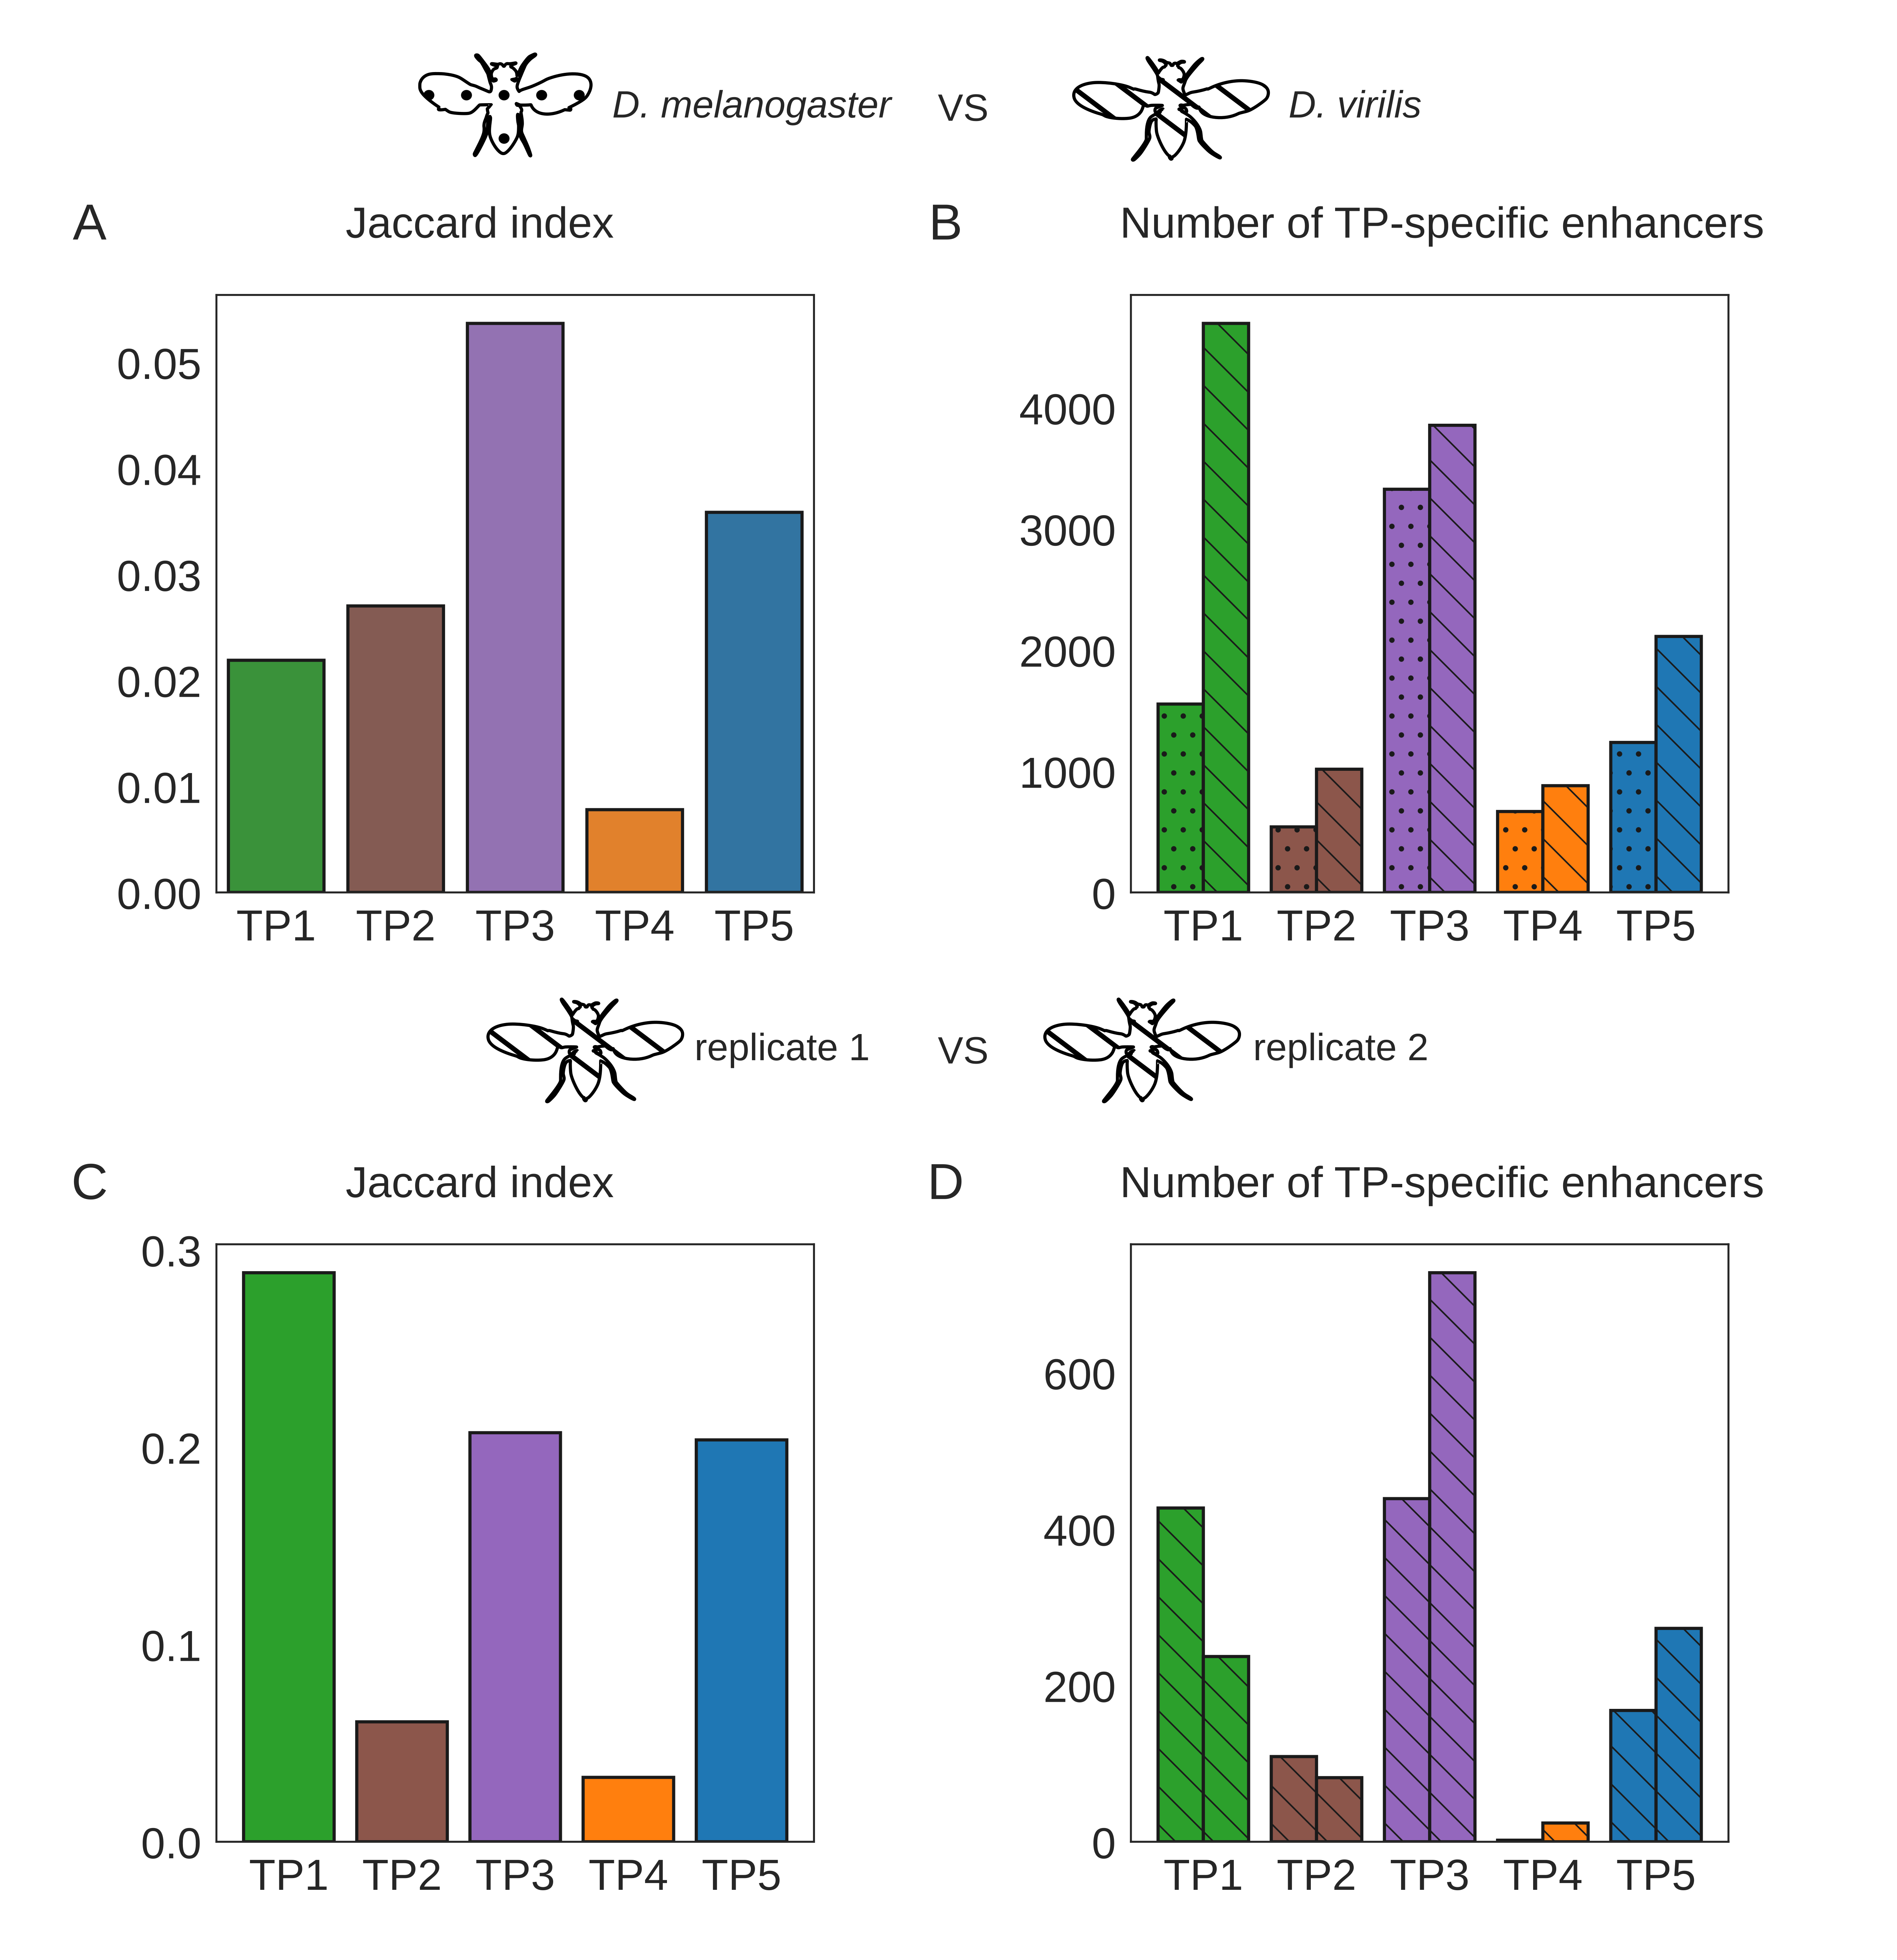
\includegraphics[width=\linewidth]{ch4.hourglass/images/fly_control_2.png}
    \caption{TODO. melanogaster vs virilis and rep1 vs rep2. Jaccard index and number of enhancers}
    \label{fig:peak_null}
\end{figure}

\begin{figure}[H]
    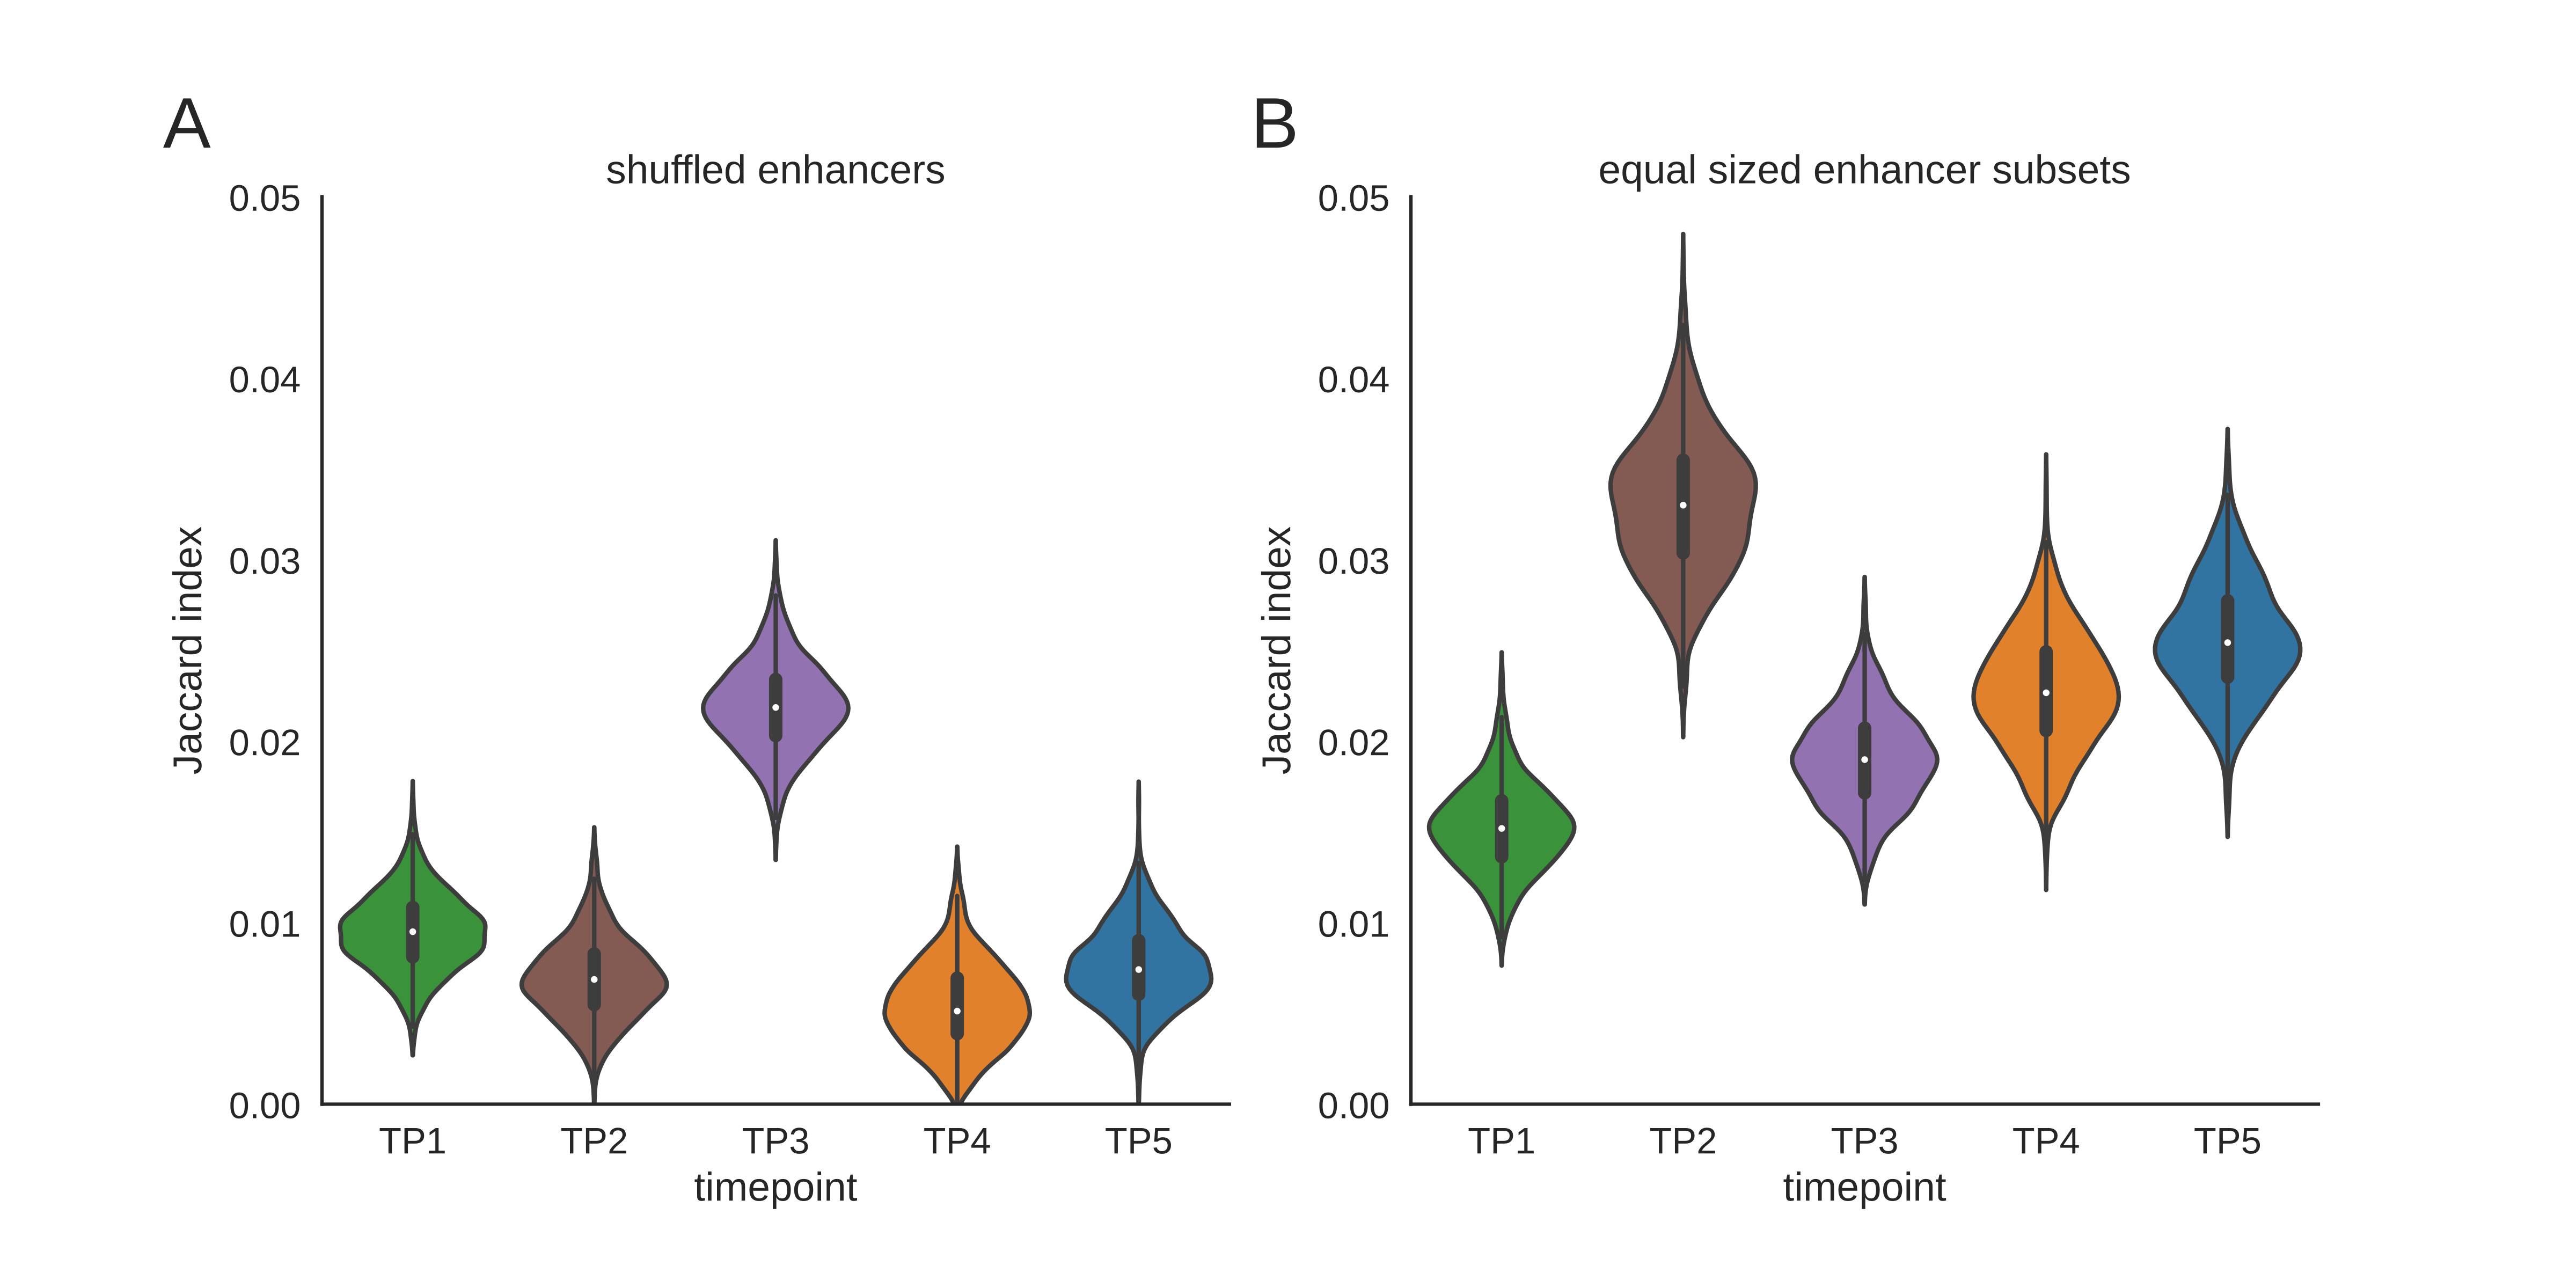
\includegraphics[width=\linewidth]{ch4.hourglass/images/fly_shuffle.png}
    \caption{shuffle explanation.}
    \label{fig:shuffle}
\end{figure}

Apart from a biological interpretation for the different number of time-point specific enhancers, there are also two methodological interpretations. Firstly, the focus on TP-specific enhancers creates artificial sets of TP-specific enhancers. TP-specific enhancers are defined as occurring in one time-point only. This means that if two time-points are sampled more closely in time than other time-points, these two time-points would share most of their enhancers, resulting in a low number of TP-specific enhancers, something the authors themselves already note. Similarly, enhancers at the beginning and the end of the time-series have a higher chance of being TP-specific purely because they are only compared against one adjacent time-point whilst the rest of the time-series are compared against two. The percentage of reads in the consensus peak set in enhancers vs promoters per time point for instance shows no clear enrichment for a specific time-point (fig. \ref{fig:peak_enrichment}). Secondly, during peak calling arbitrary thresholds are used to decide whether a region is \textit{enriched}. This threshold depends for instance on the signal-to-noise ratio, which is expected to change for a developing embryo, and the sequencing depth\cite{encode_guidelines2012}. Which neither of them have been corrected for in the original analysis.

Moreover, Liu \textit{et al.} proceed to train a computational model on the sequences of time-point specific enhancers of \textit{Drosophila melanogaster}. This model is then used to classify enhancers for whether they are subjected to positive selection. They then find that the ratio of enhancers subjected to positive selection vs enhancers subjected to non-positive selection is high for TP1, TP3, and TP5, and thus conclude that the molecular basis for the phylotypic stage can partially be explained by positive selection of gene regulation conservation. We would argue instead that there are again two likely methodological explanations to this pattern. The first explanation is that as there has been no correction for signal-to-noise ratio and sequencing depth, there is a difference in the type(s) of peaks the pre-processing picked up, which in turn translates to different predicted positive selection ratios. The second explanation is that, as is true for practically all machine learning, the model generalizes and performs better with more training data. Looking at their reported model performance (AUC) we can clearly see that the model's performance for TP1, TP3, and TP5 is notably higher than for TP2 and TP4. Looking back at figure \ref{fig:peak_null}D we see that the high model performance closely follows to the amount of training data (number of TP-specific peaks). This could simply mean that \textit{better} trained models predict a higher amount of positive selection. Without correction for these potential confounders it is hard to reach a definitive conclusion about positive selection with regards to the hourglass model and the phylotypic stage.

By comparing the within-species conservational pattern we expose important flaws in the experimental design of this study. Our re-analysis shows that the fact TP3 seems highest conserved between \textit{D. melanogaster} and \textit{D. virilis} is an effect of the number of TP-specific enhancers, and not because this time point is more conserved between these two species. Moreover it seems that the number of TP-specific enhancers also influences the downstream training of the gkm-SVM and in turn the pattern of enhancer positive selection. 

\section{Discussion}

Our study highlights the importance of including within-species, within-phylum and between-phylum comparisons in the analysis of the phylotypic stage. We demonstrate that the high transcriptome similarity between \textit{D. rerio} and \textit{X. tropicalis} at the phylotypic stage can be explained by within-species effects alone. Furthermore, we identify the mid-developmental transition and \textit{Drosophila} enhancer conservation at the phylotypic stage as statistical artefacts. 

When comparing time-series directly, it is important to control for statistical biases in the data, such as the correspondence between replicates, but also the temporal sampling strategy, data distribution, cell type proportion and gene sets used. A key bias that is often overlooked is whether the sampling schema follows developmental time\cite{BinindaEmonds2002}. It is not uncommon for studies to report a discontinuous blocked pattern of within-species conservation, where the difference between stages is not equal. This difference often gets assigned a biological explanation; for instance as embryonic genome activation\cite{Yanai2011} or developmental milestones\cite{Levin2012}. However, this blocked within-species pattern proceeds to affect the between-species comparison where the same blocks are visible. From a data science point of view, the only way to make a fair comparison between time series is when the similarity between all adjacent time points is equal (or if one explicitly corrects for this bias statistically). When sampling stages closely in time, one increases the probability of stages to match closely in a comparison with another time-series. This in turn increases the expected maximum similarity. The reverse is also true, where stages sampled in large intervals reduces the probability of matching stages between time-series, which then reduces the expected maximum similarity. Thus under the assumption that embryonic development has no point of higher selective pressure, a comparison between two time-series will have the highest expected similarity at the point where sampling has happened at the shortest interval. For this reason we argue for a re-definition of molecular embryonic time, where not morphological features or time post fertilisation is used, but where the (molecular) difference between adjacent stages is equal.

Similarly, changing gene expression distributions are an effect of developmental maturity\cite{Kannan2021}. Pluripotent tissues have relatively many genes activated, whilst more mature tissues make use of a smaller more specialized set of genes. These changing gene expression distributions over time can introduce unexpected biases and artefacts when calculating similarity. For instance, the JSD and Pearson correlation coefficient between two count tables from different distributions can respectively never be zero or one. As an effect, directly comparing similarity scores between time-points can be misleading as the range of possible similarity scores is different per comparison. To circumvent this problem one can resort to non-parametric distance metrics, such as the rank-based Spearman correlation coefficient\cite{Irie2011}, or quantile normalizing the data before calculating the distance metric\cite{marletaz2018}. Then, one can compare the similarity scores directly, but these approaches ignore the biologically relevant gene expression distribution changes. As long as there is no consensus on what type of molecular similarity is expected at the phylotypic stage, it can both be correct as well as incorrect to ignore the distributional changes. 

Another point to consider is the changing proportions of cell types. An embryo is formed by all the multiplying and developing cells together, and their combined signal is measured in the study of the molecular phylotypic stage. But not every cell type expresses the same amount of transcripts\cite{Kim2023, Percharde2017}, which consequently gives cells with a lot of transcripts a higher importance in the (dis)similarity calculation. Moreover, changes in similarity between species could be either caused by changes in gene expression, or by changes in cell proportions. For example, during the vertebrate phylotypic stage the neural tissue is already highly developed and relatively large. Perhaps similarity at the vertebrate phylotypic stage is an effect of the over-representation of these neural cell types. Or as another example, a practically universal feature of embryos is that they grow during development. But because of this growth, for example, the surface (skin) to volume (organs) ratio changes, which could be another driving force for the molecular phylotypic stage. We currently do not understand whether the molecular similarity at the phylotypic is based on a similarity on cell type proportion similarity or whether it is based on gene expression similarity. Mayshar \textit{et al.} compared the cell type proportions over time of developing mouse and rabbit embryos. They encounter the same statistical artefact as Levin \textit{et al.} in their mid-developmental transition paper, but surprisingly, and wrongly, conclude they find an hourglass pattern\cite{Mayshar2023}. Nevertheless, a single-cell approach can distinguish the effects of cell type proportion and gene expression, which is essential for better understanding the molecular phylotypic stage.

Moreover, calculating a single similarity score between species seems like a gross oversimplification of the complexity of evolutionary development. When focusing on one-to-one orthologues features, all newly derived and features are ignored. For instance, we started our analysis with 21.154 genes for \textit{X. tropicalis} and 24.417 genes for \textit{D. rerio} respectively. However, if we focus only on one-to-one orthologs this gets reduced to 5.444 one-to-one orthologous genes. This means that for this comparison specifically we ignore approximately three-quarters of the data. To our knowledge the only method that considers these relations is the transcriptomic derivedness index\cite{Leong2021}. Moreover, gene expression is regulated by the complex interplay of multiple gene regulatory mechanisms. For instance, a single differentially expressed transcription factor can affect thousands of downstream genes. Biological data is notoriously not independently and identically distributed (iid). Whole-transcriptome comparisons are thus biased towards the largest groups of co-regulated genes. In addition, the fact that comparisons subsetted on different GO terms result in different conservational patterns is a clear indication that a single metric for whole-transcriptome similarity conceals the different layers of conservation at the phylotypic stage\cite{Malik2017,Gildor2019,Onimaru2021}.

Even though there has been extensive research into the molecular basis of the phylotypic stage, there is currently no clear hypothesis for it. There is no pre-defined expectation when comparing between members of different phyla, nor has it been defined whether similarity between species of the same phylum is a between-species or within-species effect. It is unclear whether high similarity is expected as a generic gene expression similarity(dynamic pattern), or whether the high similarity expresses itself as highly conserved gene regulation(gene regulatory complexity). Without testing these comparisons we can not fully appreciate and understand the complexity of evolutionary embryonic development. Moreover, we do not feel that the current whole-embryo pairwise comparisons are a sincere attempt to understand evolutionary development, but instead are applied just because they are simplest to measure. 

\section{Material and Methods}

The final analysis can be found on \url{https://github.com/vanheeringen-lab/phylotypic\_hourglass}.

\subsection{Transcriptome analyses}

Preprocessing of RNA-seq was done automatically by seq2science v0.9.8\cite{seq2science} using the rna-seq workflow. Public samples were downloaded from the Sequence Read Archive with help of the ncbi e-utilities and pysradb\cite{Choudhary2019}. Genome assemblies UCB\_Xtro\_10.0 (\textit{X. tropicalis}), GRCz11 (\textit{D. rerio}), BDGP6.32 (\textit{D. melanogaster}), ce11 (\textit{C. elegans}) and GRCm38.p6 (\textit{M. musculus}) were downloaded with genomepy 0.13.0\cite{Frlich2023}. Reads were trimmed with fastp v0.20.1\cite{Chen2018} with default options. Reads were aligned with STAR v2.7.6a\cite{Dobin2012} with default options. Afterwards, duplicate reads were marked with Picard MarkDuplicates v2.23.8\cite{picard}. General alignment statistics were collected by samtools stats v1.14\cite{Danecek2021}. Read counting and summarizing to gene-level was performed on filtered bam using HTSeq-count v0.12.4\cite{Anders2014}. TPM normalized gene counts were generated using genomepy based on longest transcript lengths. Quality control metrics were aggregated by MultiQC v1.14\cite{Ewels2016}. 

The within-species permutation test was performed by randomly choosing two replicates of the same time-point and calculating their Spearman correlation coefficient, with per time point 250 random pairs.

Orthologs between species were derived by the gimmemotifs motif2factors command. This command downloaded the genome assemblies of TODO X Y Z through genomepy\cite{Frlich2023}, and converted all transcripts to peptides with gffread 0.12.7\cite{Pertea2020}. Only the longest peptide per gene was kept, which were then fed to orthofinder 2.5.4\cite{Emms2019}.

For the re-analyses we then took the average TPM per time point, kept per species-species comparison only the one-to-one orthologs, and did similar processing as the original studies. Specifically for the re-analysis of Marl\'etaz \textit{et al.} we quantile normalized\cite{qnorm} the TPMs and calculated the Jensen-Shannon distance on a log2 scale with TPMs divided by a million. For the re-analysis of Levin \textit{et al.} we removed all genes with a minimum TPM lower than 10 and less than a 10-fold change. Then we log10 transformed the remaining data and calculated the Pearson correlation coefficient.

\subsection{Enhancer conservation}

We've had troubles closely reproducing the original results of Liu \textit{et al.}, so we've opted to use the original processed data for the between-species comparison, but our own processed data for the within-species comparisons as this data is missing. By closely reproducing the original results with their data it shows that our ortholog inference works similar to theirs.

Preprocessing of the within-species comparisons was done automatically by seq2science v0.9.8\cite{seq2science} using the atac-seq workflow\cite{Choudhary2019}. Genome assemblies \textit{dm6} and \textit{droVir3} were downloaded with genomepy 0.13.0\cite{Frlich2023}. Paired-end reads were trimmed with fastp v0.20.1\cite{Chen2018} with default options. Reads were aligned with bwa-mem2 v2.2.1\cite{bwamem2} with options '-M'. Afterwards, duplicate reads were marked with Picard MarkDuplicates v2.23.8\cite{picard}. Before peak calling, paired-end info from reads was removed with seq2science so that both mates in a pair get used. The peak-calling effective genome size was estimated by khmer v2.0\cite{Crusoe2015} by calculating the number of unique k-mers with k being the average read length per sample. Peaks were called with macs2 v2.2.7\cite{Zhang2008} with options '--shift -100 --extsize 200 --nomodel --buffer-size 10000' in BAM mode. A consensus set of all summits was made with gimmemotifs 0.17.2\cite{gimmemotifs}. We've removed all summits that fall within a TSS with pyranges v0.0.120\cite{Stovner2019}.

For the between-species comparison we've used pslmap to map all \textit{droVir3} enhancers to the \textit{dm6} assembly and only kept one-to-one orthologous regions. For the within-species comparisons this is not necessary. Time-point specific enhancers are defined as enhancers of which the summits are more than 200 base pairs removed from the enhancers of other time-points. Overlap over time is calculated as the Jaccard index.

\section{Acknowledgements}

We would like to thank Jialin liu for his quick response on queries about the \textit{Drosophila} transcriptome datasetm, Eileen Furlong for her help with processing the DNAse \textit{Drosophila} samples, Michal Levin and Itai Yanai for sharing their original orthology dataset, David Emms for help with questions about orthofinder. Mike Keesey for developing Phylopic, and Eivind Fonn for his help with formalizing the mathemathical derivations.

\section{Supplementals}

\subsection{mid-developmental transition derivation}\label{subsection:middevelopmenttransition}

A basic proof that the mid-developmental transition is a methodological artefact follows relatively easily from the thought experiment where a gene starts the time-series in an \textit{off} state, and at random switches to an \textit{on} state somewhere along this time-series:

\begin{align*}    
    G(t) & = \begin{cases} \text{off},& t < t_{\text{activate}} \\ \text{on},& t \geq t_{\text{activate}} \end{cases} \quad \textrm{and} \quad
    t_{\text{activate}} = \text{Uniform}(0, 1) \quad \textrm{and} \quad
    0 \leq t \leq 1
\end{align*}

then:

\begin{align*}
    P(G(t) & = \text{on}) = t \\
    P(G(t) & = \text{off}) = 1 - t
\end{align*}

If we now assume we have two of these time-series (x and y), we can define the probabilities that both genes are in the same state for $t_x$ and $t_y$:

\begin{align*}
    P(G(t_x) = G(t_y)) & = P(G(t_x) = \text{on}) \cdot P(G(t_y) = \text{on}) + P(G(t_x) = \text{off}) \cdot P(G(t_y) = \text{off}) \\
    & = t_x \cdot t_y + (1 - t_x) \cdot (1-t_y)
\end{align*}

When visualizing the probability for equality over all x and y a mid-developmental transition becomes clear (fig. \ref{fig:inverse_math}).

\subsection{Jaccard index}\label{subsection:flypeaks}

We assume that all enhancers are conserved between species $x$ and $y$. Moreover we assume that our pre-processing randomly finds enhancers for each time-point with chance $\alpha_{ts}$, where $t$ represents the time-point and $s$ represents the species. We can calculate the number of time-point specific peaks for $U_{ts}$ in this case as:

\begin{align*}
    E & \text{ is the collection of all conserved enhancers between species } x \text{ and } y \\
    U_{ts} & \text{ represents the time-point specific enhancers for species } s \text{ at time point } t \\
    |U_{ts}| & = \alpha_{ts} \beta_{ts} |E|, \text{ where } \beta_{ts} = \prod_{i \in \{1, 2, 3, 4, 5\}\setminus\{t\}} (1 - \alpha_{is}) \\
\end{align*}

Where $\beta_{ts}$ represents the fraction of enhancers that have are still eligible to be time-point specific. We can now calculate the expected overlap (union) between two time-points of species $x$ and $y$:

\begin{align*}
    \mathbb{E}(|U_{tx} \cap U_{ty}|) & = |U_{tx}| * \frac{|U_{ty}|}{|E|} \\
    & = \alpha_{tx} \beta_{tx} |E| * \frac{\alpha_{ty} \beta_{ty} |E|}{|E|} \\
    & = \alpha_{tx} \beta_{tx} \alpha_{ty} \beta_{ty} |E| \\
\end{align*}

From this we can calculate the expected Jaccard index:

\begin{align*}
    Jaccard(U_{tx}, U_{ty}) & = \frac{|U_{tx} \cap U_{ty}|}{|U_{tx} \cup U_{ty}|} \\
    & = \frac{|U_{tx} \cap U_{ty}|}{|U_{tx}| + |U_{ty}| - |U_{tx} \cap U_{ty}|} \\
    & = \frac{\alpha_{tx} \beta_{tx} \alpha_{ty} \beta_{ty} |E|}{(\alpha_{tx} \beta_{tx} + \alpha_{ty} \beta_{ty} - \alpha_{tx} \beta_{tx} \alpha_{ty} \beta_{ty})|E|} \\
    & = \frac{\alpha_{tx} \beta_{tx} \alpha_{ty} \beta_{ty}}{\alpha_{tx} \beta_{tx} + \alpha_{ty} \beta_{ty} - \alpha_{tx} \beta_{tx} \alpha_{ty} \beta_{ty}}
\end{align*}

For simplicity we assume that all found enhancers are time-point specific ($\beta_{ts} = 1$), simplifying the formula to:

\begin{align*}
    Jaccard(U_{tx}, U_{ty}) & = \frac{\alpha_{tx} \alpha_{ty}}{\alpha_{tx} + \alpha_{ty} - \alpha_{tx} \alpha_{ty}}
\end{align*}

We can now visualize the Jaccard index for different $\alpha_{ts}$ values and can see a clear dependence on the fraction of enhancers found and the Jaccard index (fig. \ref{fig:peak_math}). From this it is clear that we need to correct for the number of enhancers. $\beta_{ts}$ only influences the height of the Jaccard index, but not the pattern.

\subsection{supplemental figures}
\beginsupplement

\begin{figure}[H]
    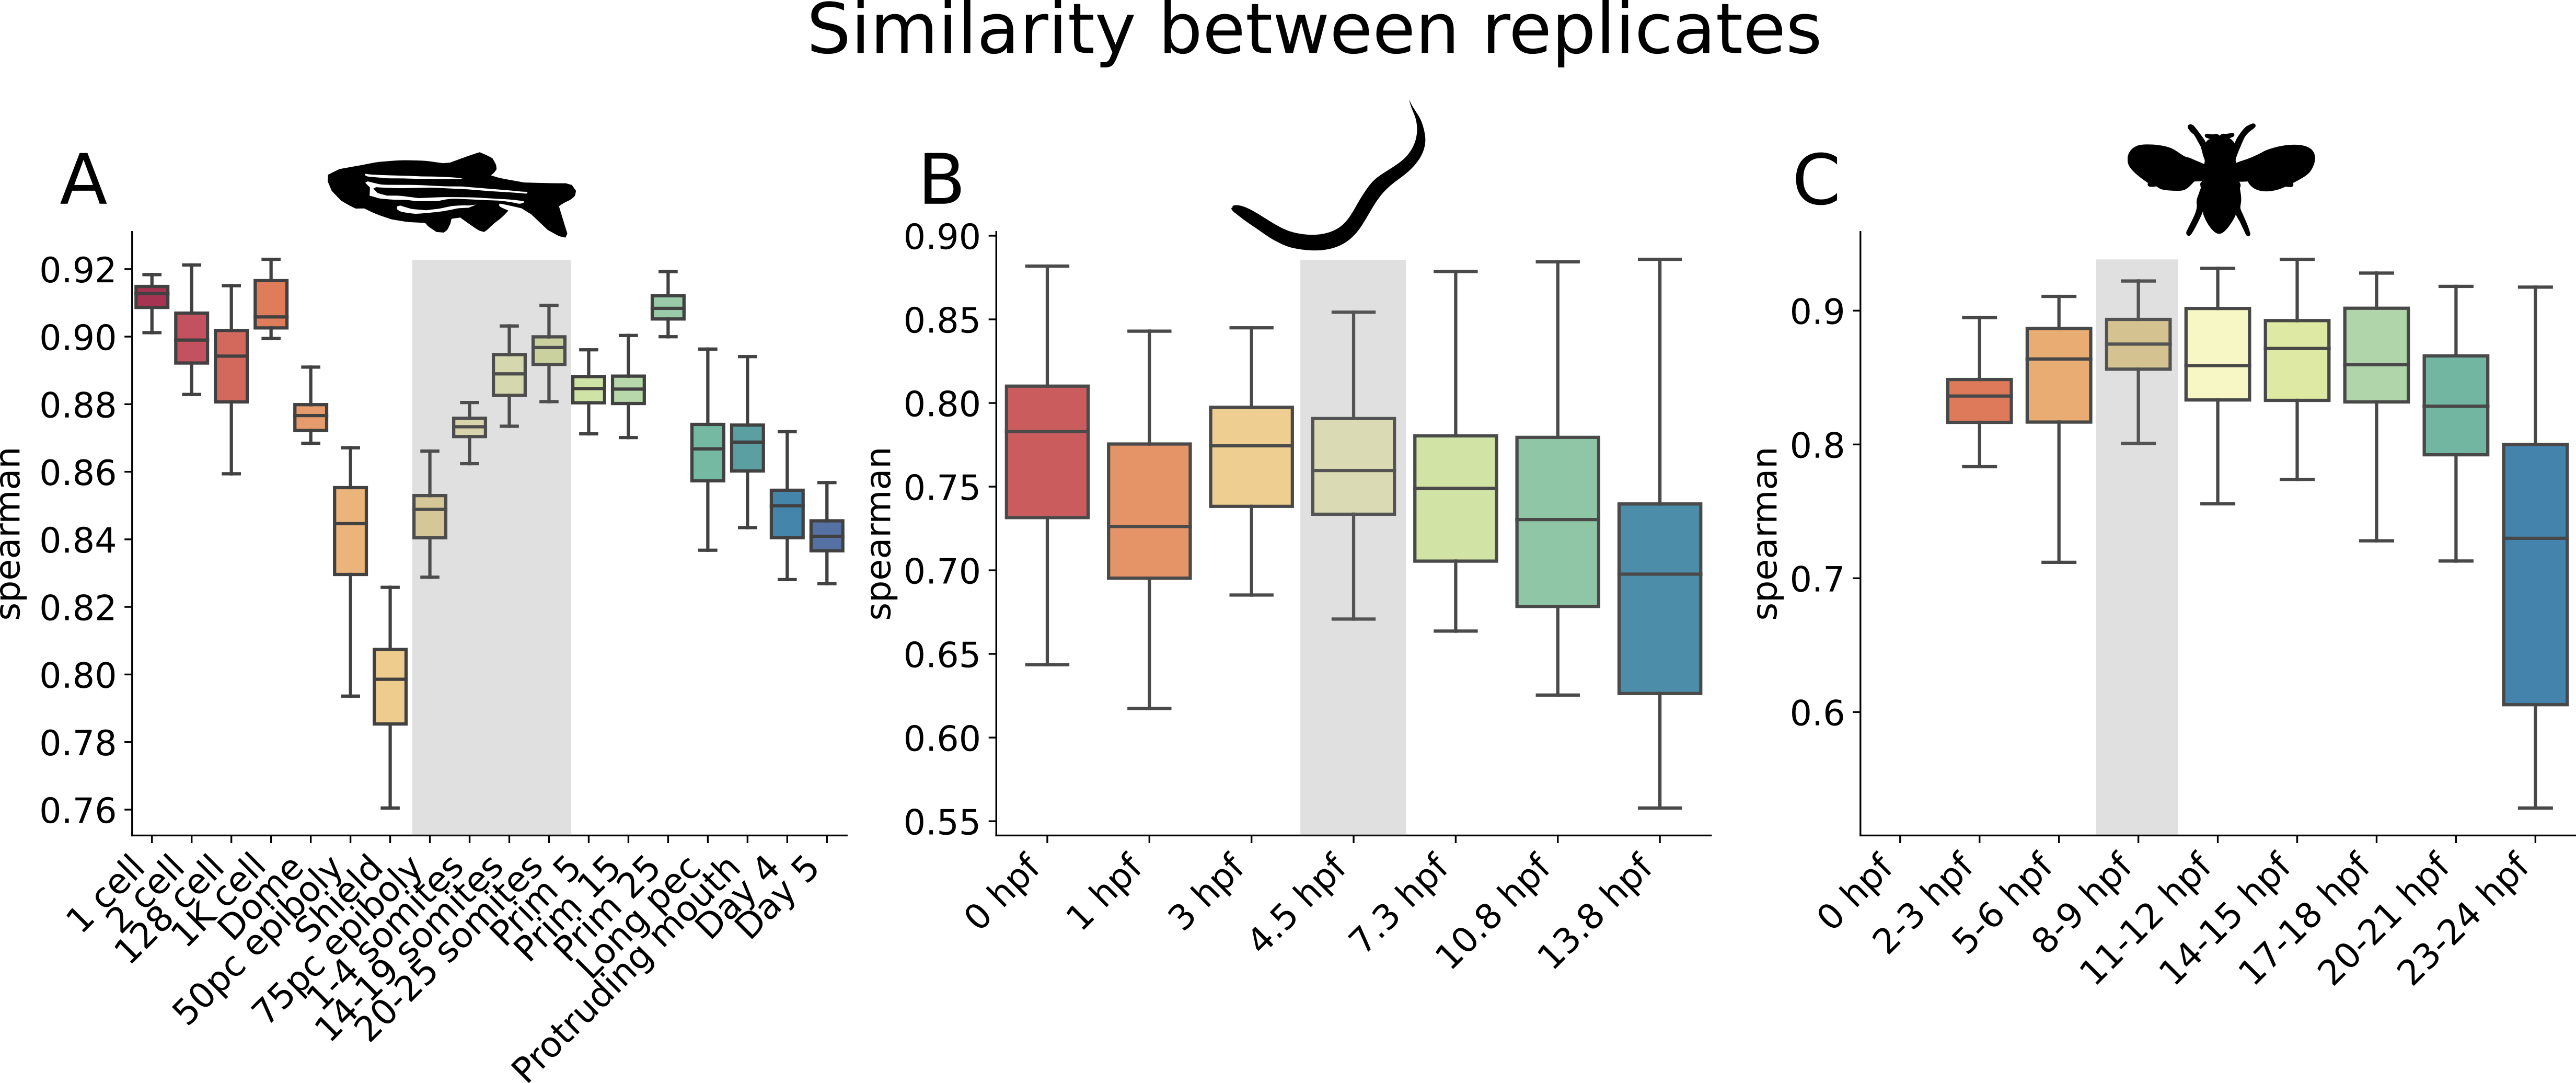
\includegraphics[width=\linewidth]{ch4.hourglass/images/within_timepoint.png}
    \caption{Distribution of gene expression spearman correlation coefficient between replicates belonging to the same stage for (A) single embryo \textit{D. rerio} samples, (B) pools of 10 \textit{C. elegans} embryos, and (C) single-embryo \textit{D. melanogaster} samples. Distribution consists of 250 pairs randomly sampled. The shaded area indicates the phylotypic stage. }
    \label{fig:within_timepoint}
\end{figure}

\begin{figure}[H]
    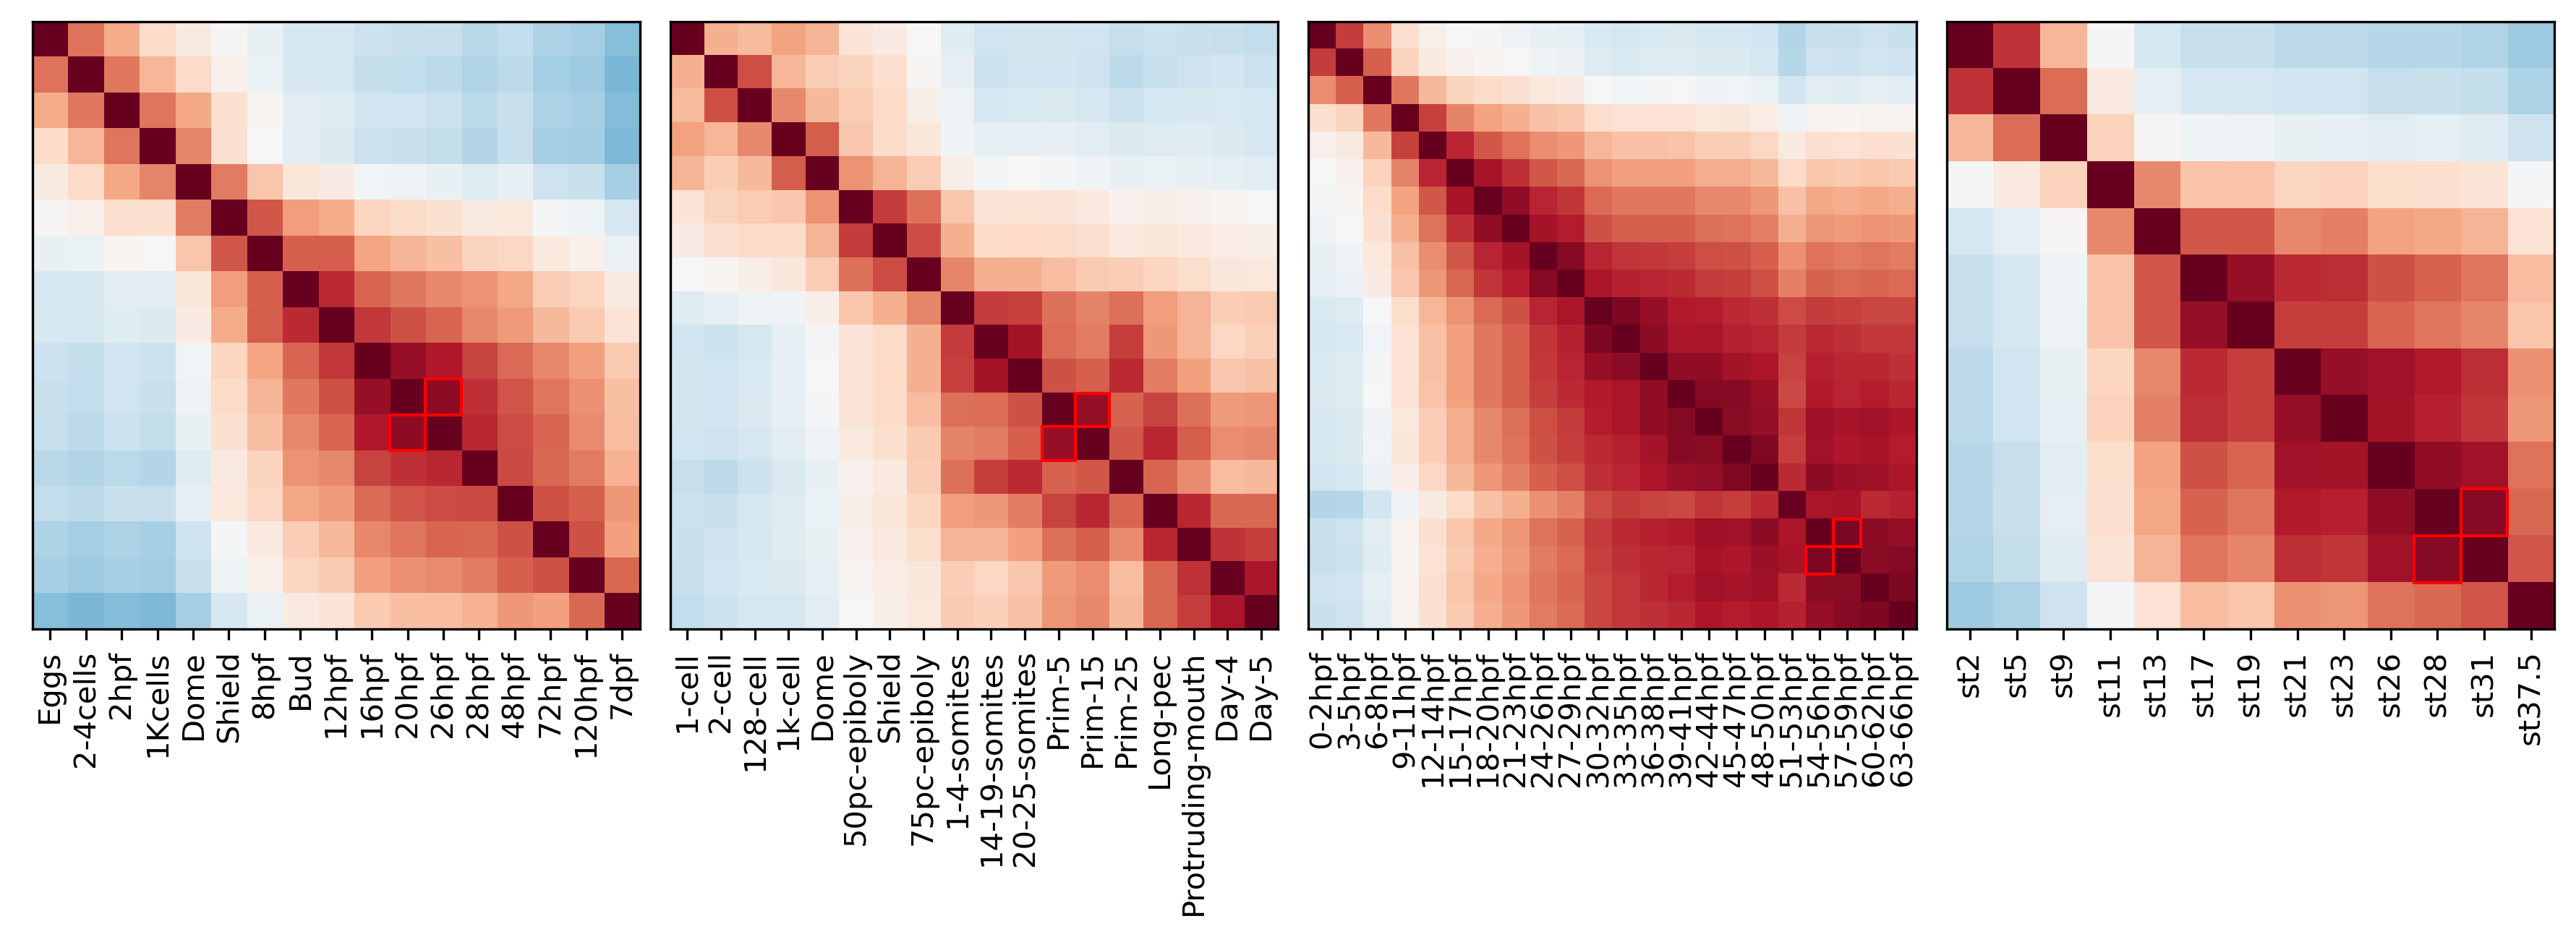
\includegraphics[width=\linewidth]{ch4.hourglass/images/within_species.png}
    \caption{Self-correlation of different}
    \label{fig:withinspecies}
\end{figure}

\begin{figure}[H]
    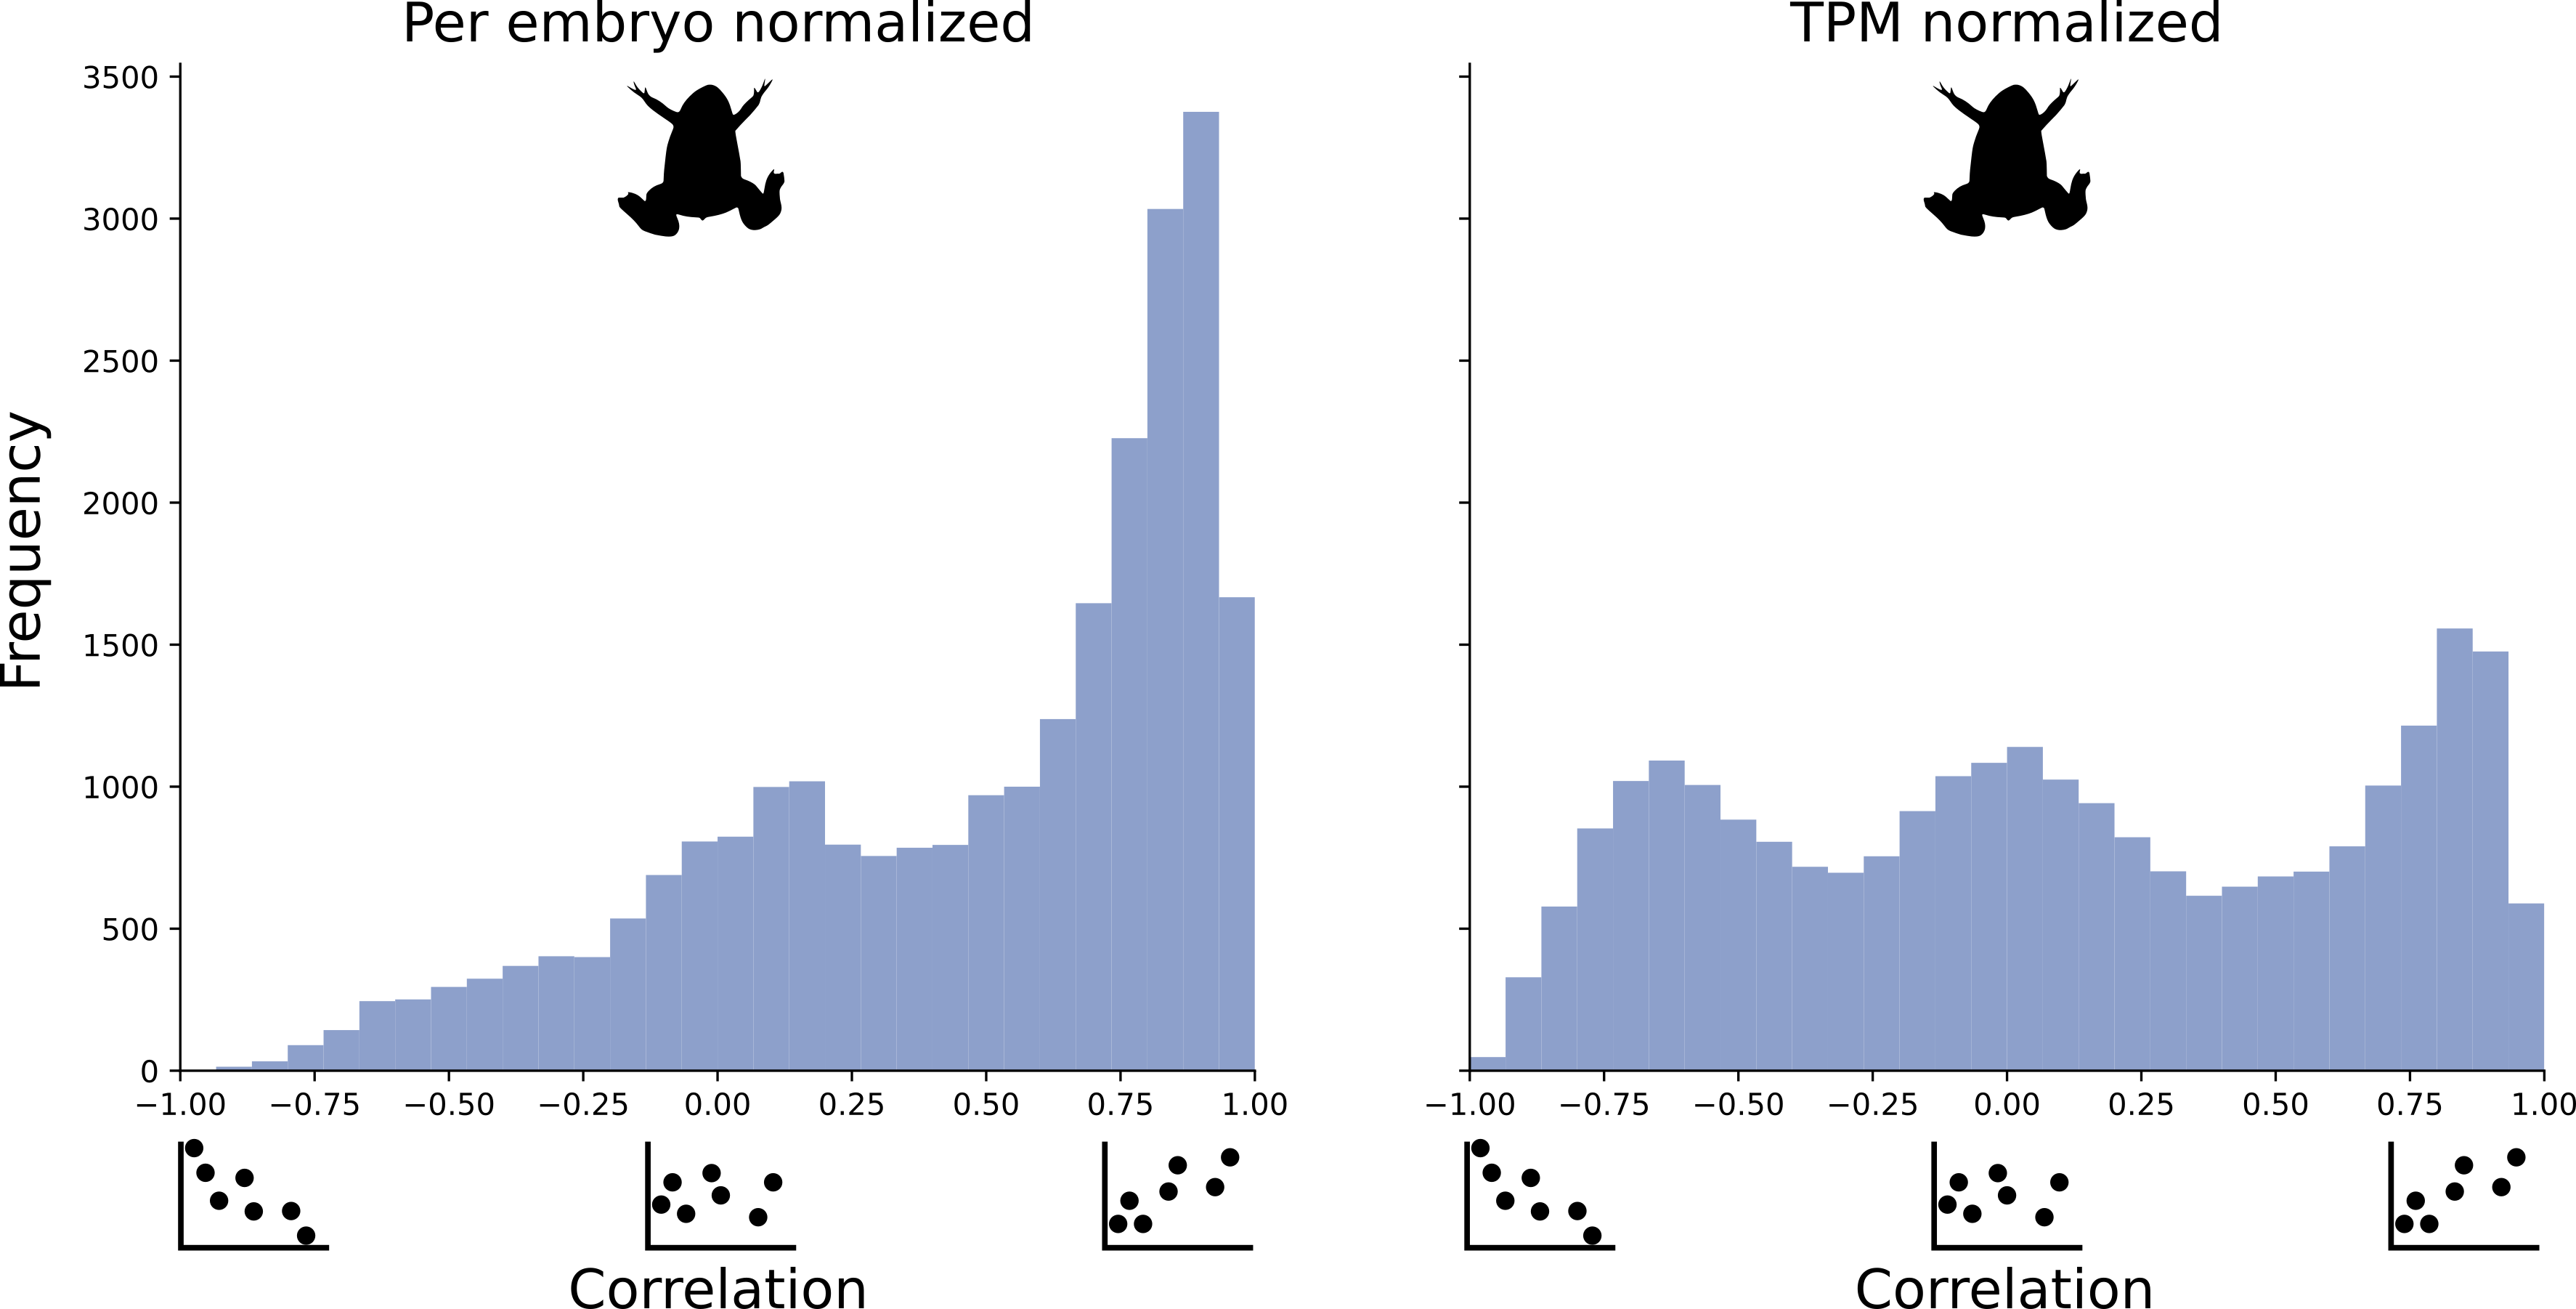
\includegraphics[width=\linewidth]{ch4.hourglass/images/gene_landscape_normalization.png}
    \caption{The difference in gene landscape between per-embryo normalization and TPM normalization of \textit{X. tropicalis}. Figure A shows the gene landscape of per-embryo normalized gene expression. Because the \textit{X. tropicalis} embryo grows practically all genes are upregulated on a per-embryo basis. In panel B the gene landscape of TPM normalized gene expression is visualized. Here we see that there are roughly three groups of gene expression, a down-regulated, a constant, and an up-regulated group. TODO add A and B}
    \label{fig:genelandscapenormalization}
\end{figure}

\begin{figure}[H]
    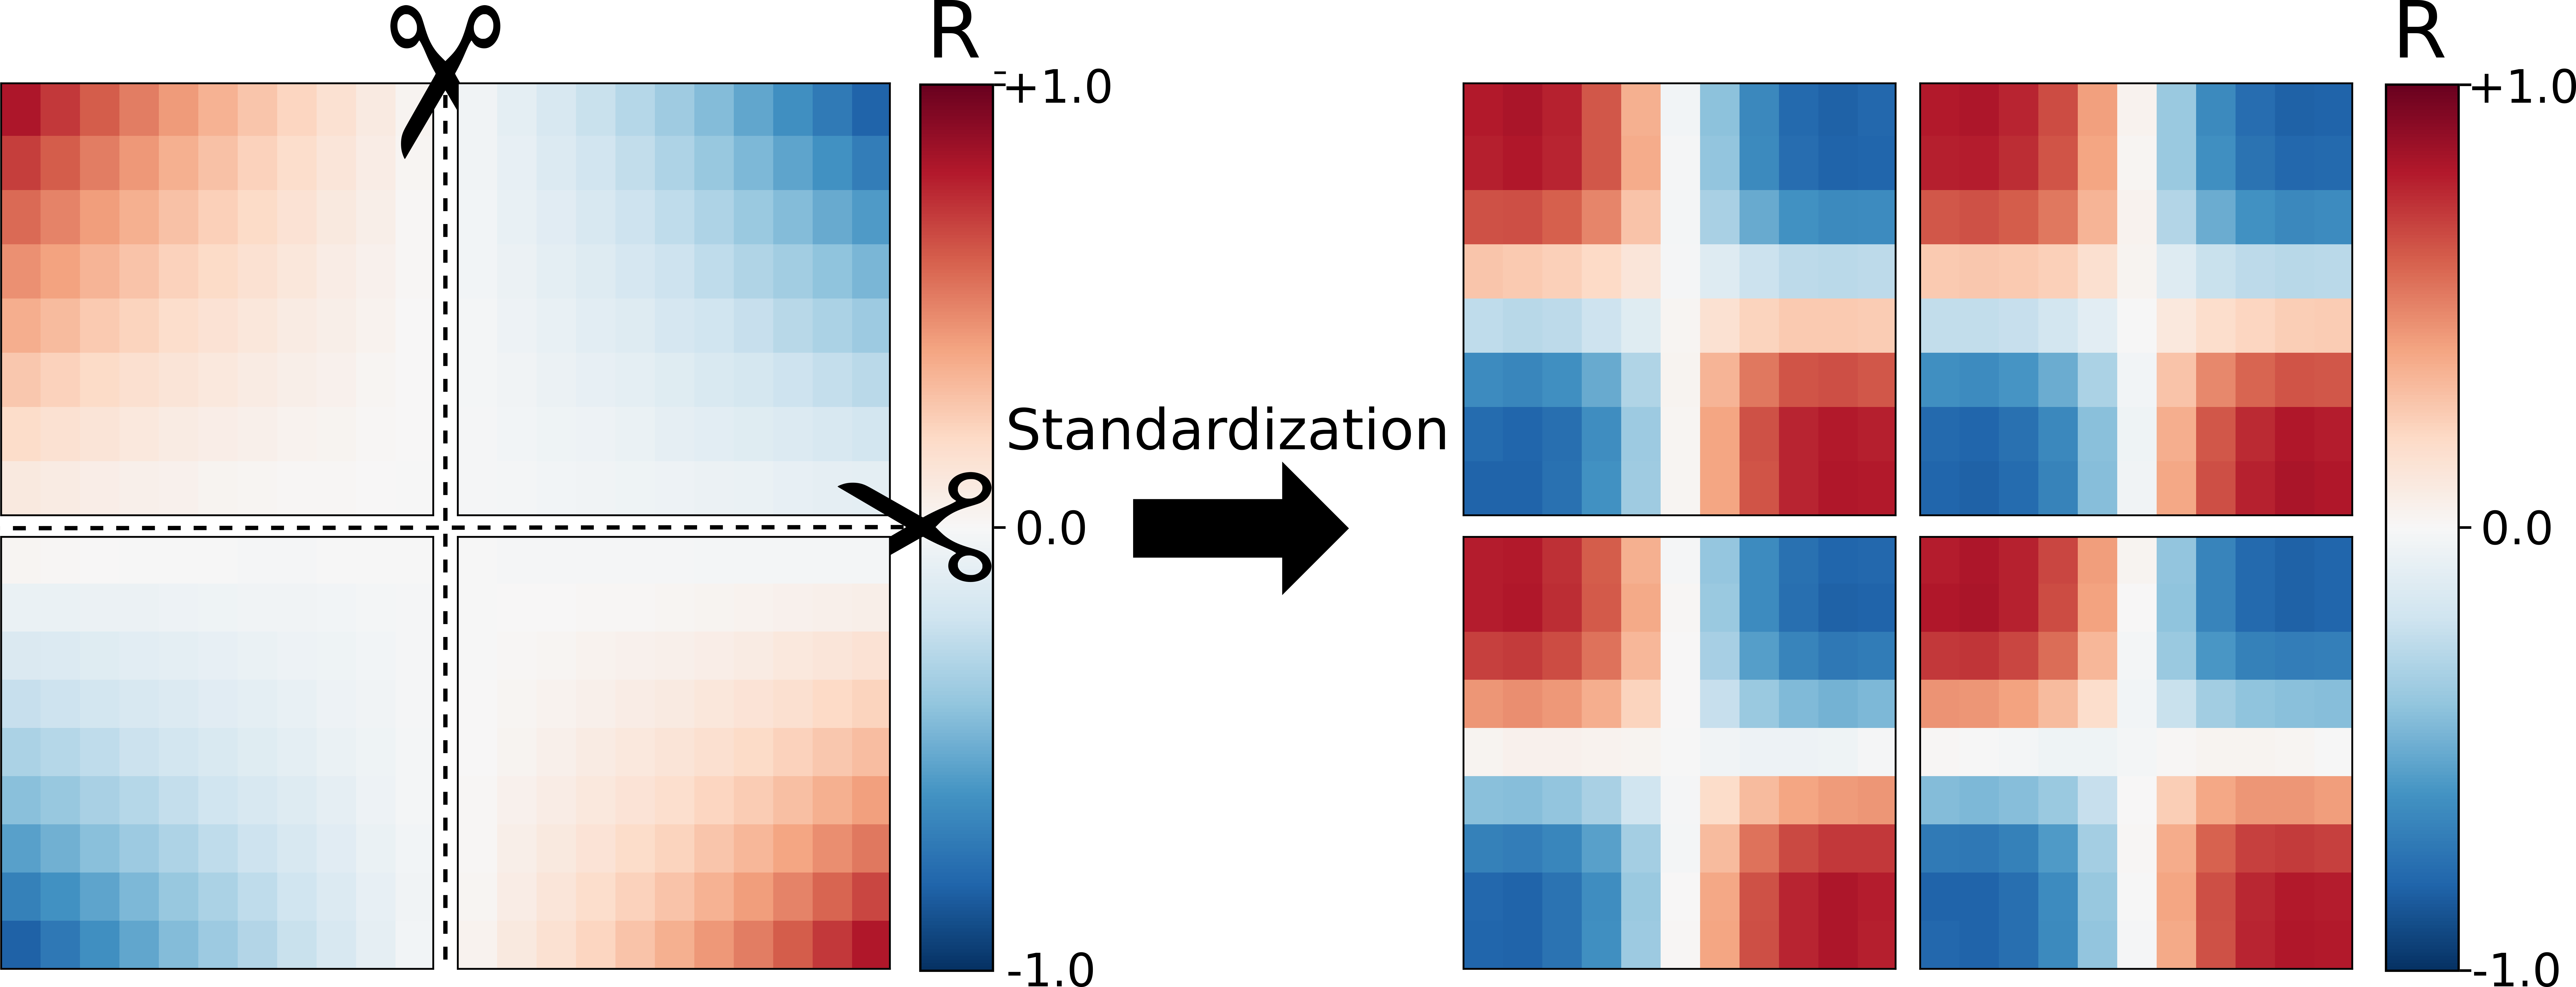
\includegraphics[width=\linewidth]{ch4.hourglass/images/sim_normalisation.png}
    \caption{Cutting the simulated data set into four quarters and applying standardization afterwards results in an inverse hourglass for each quarter.}
    \label{fig:sim_normalisation}
\end{figure}

\begin{figure}[H]
    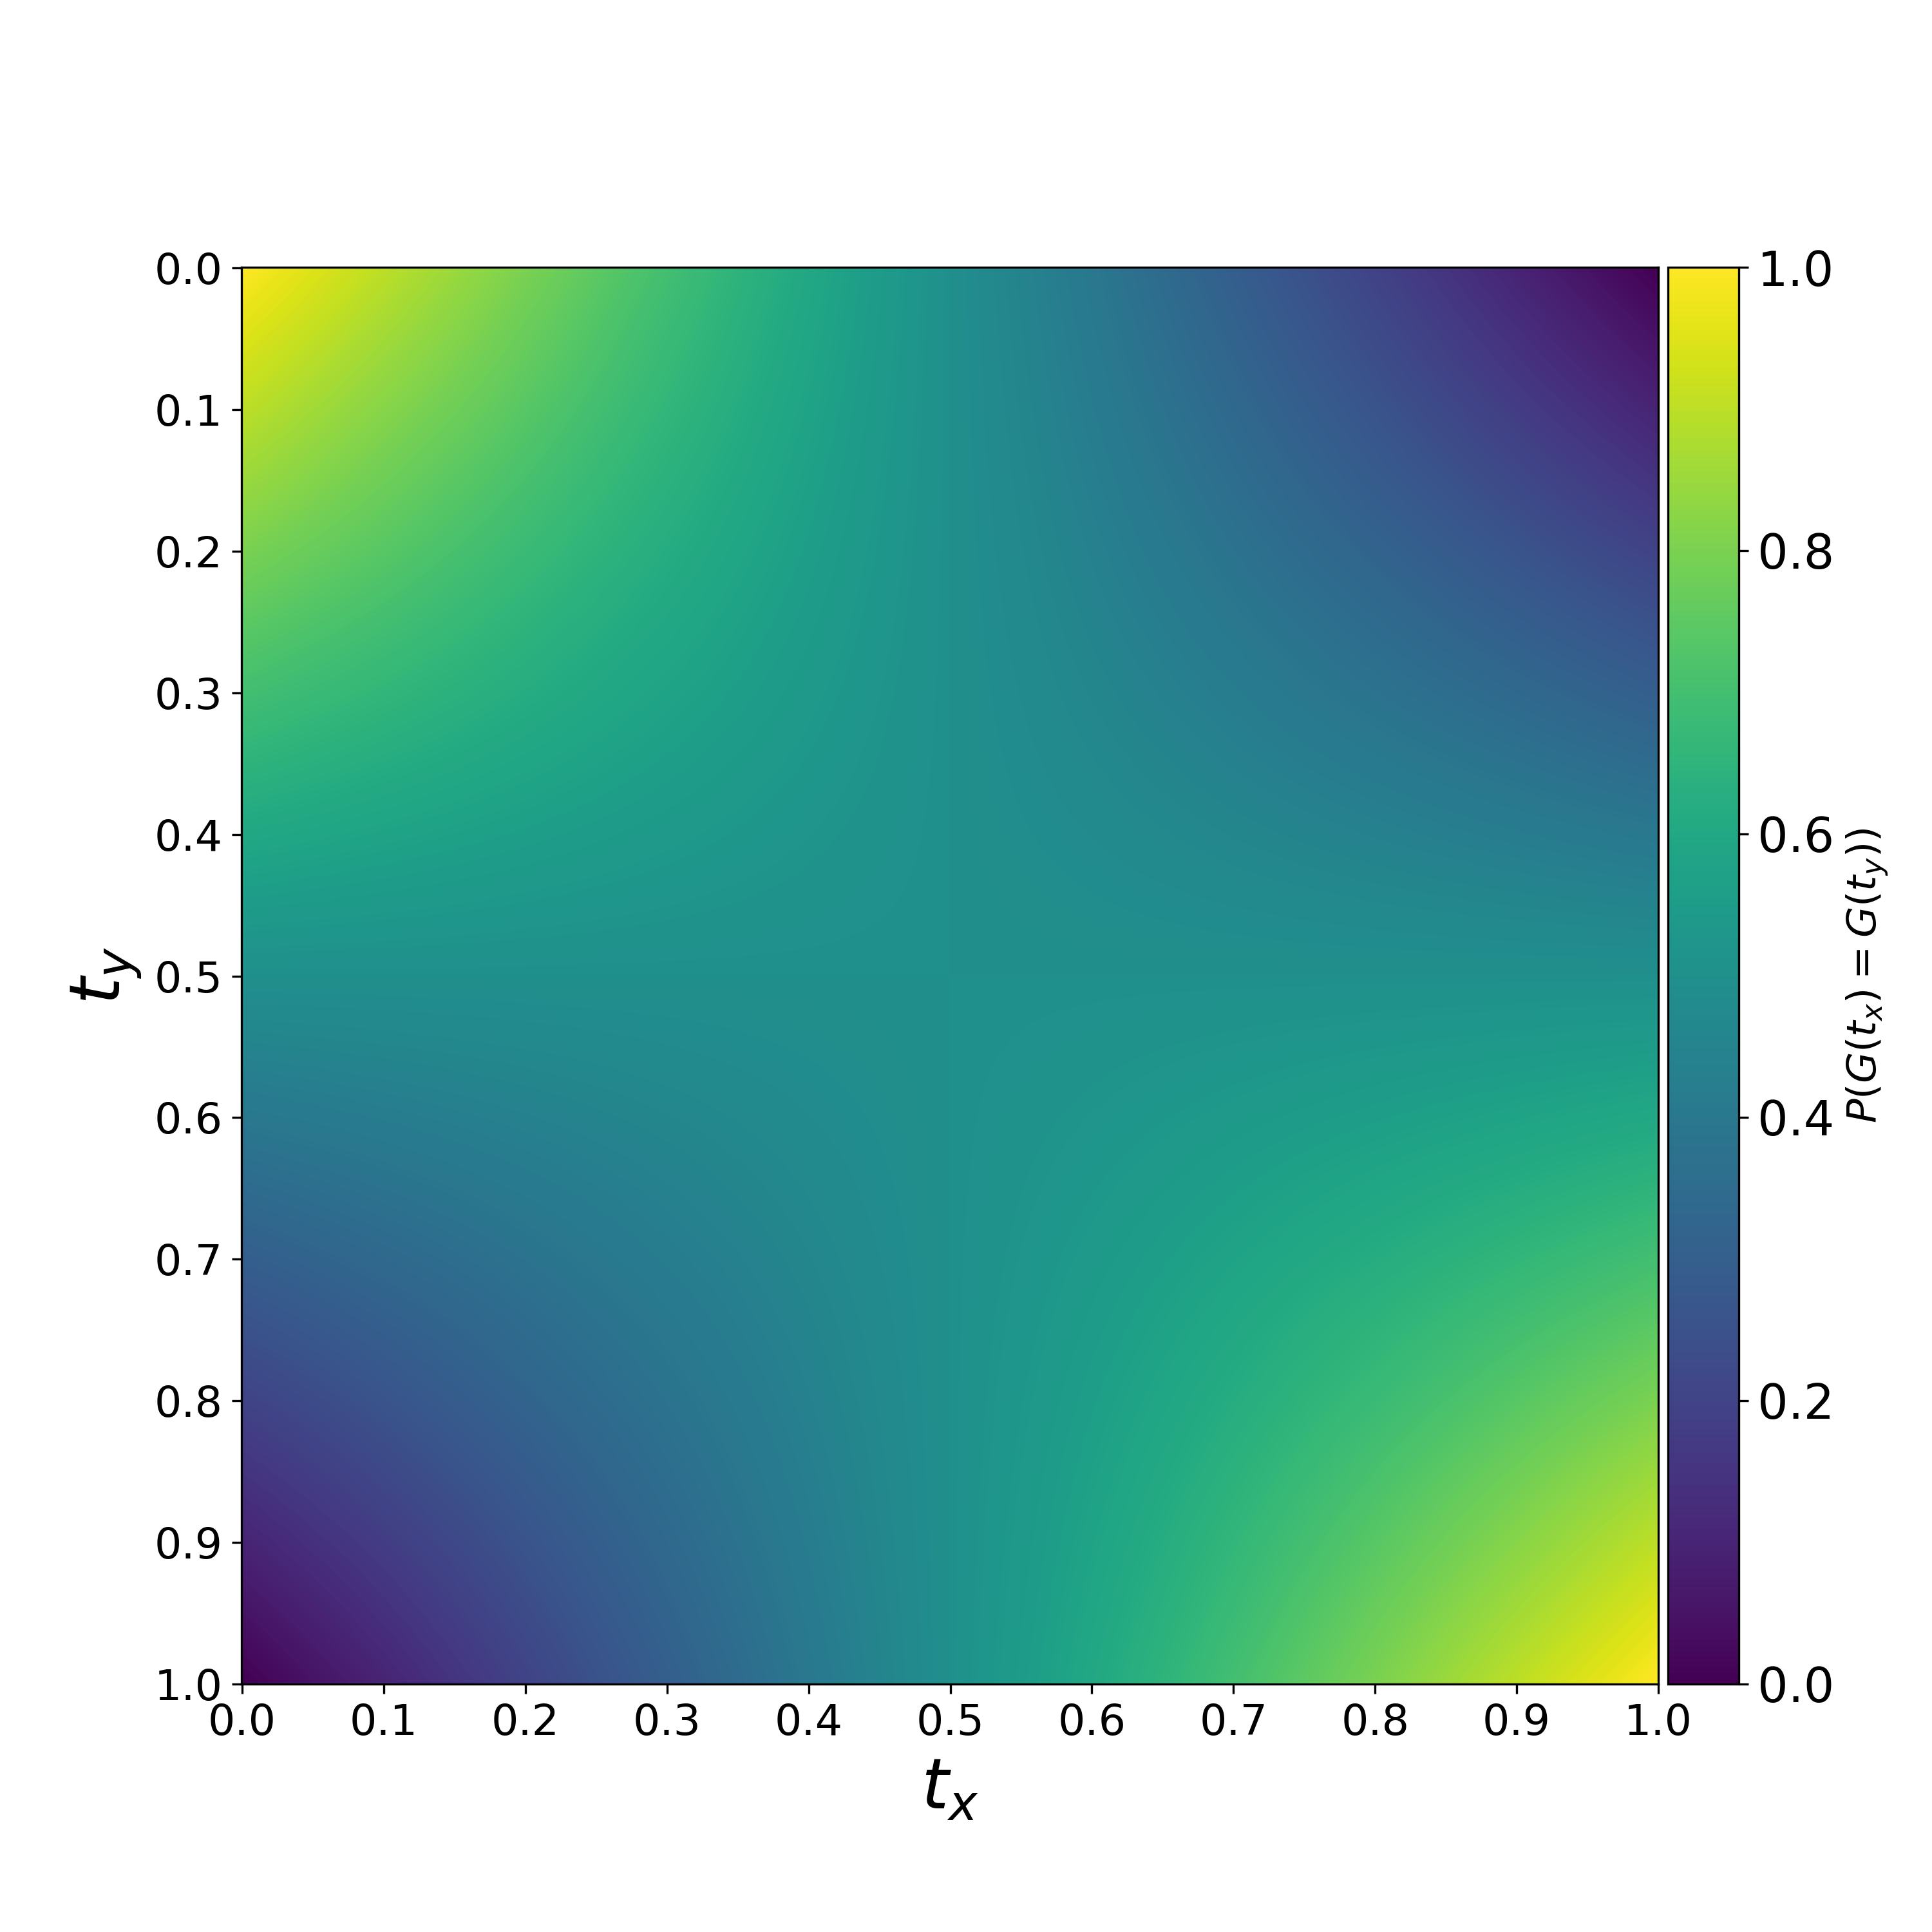
\includegraphics[width=\linewidth]{ch4.hourglass/images/math_inverse.png}
    \caption{The probability that two variables are equal under the assumption that they both start \textit{off} and end \textit{off}, but their moment of switching is random.}
    \label{fig:inverse_math}
\end{figure}

\begin{figure}[H]
    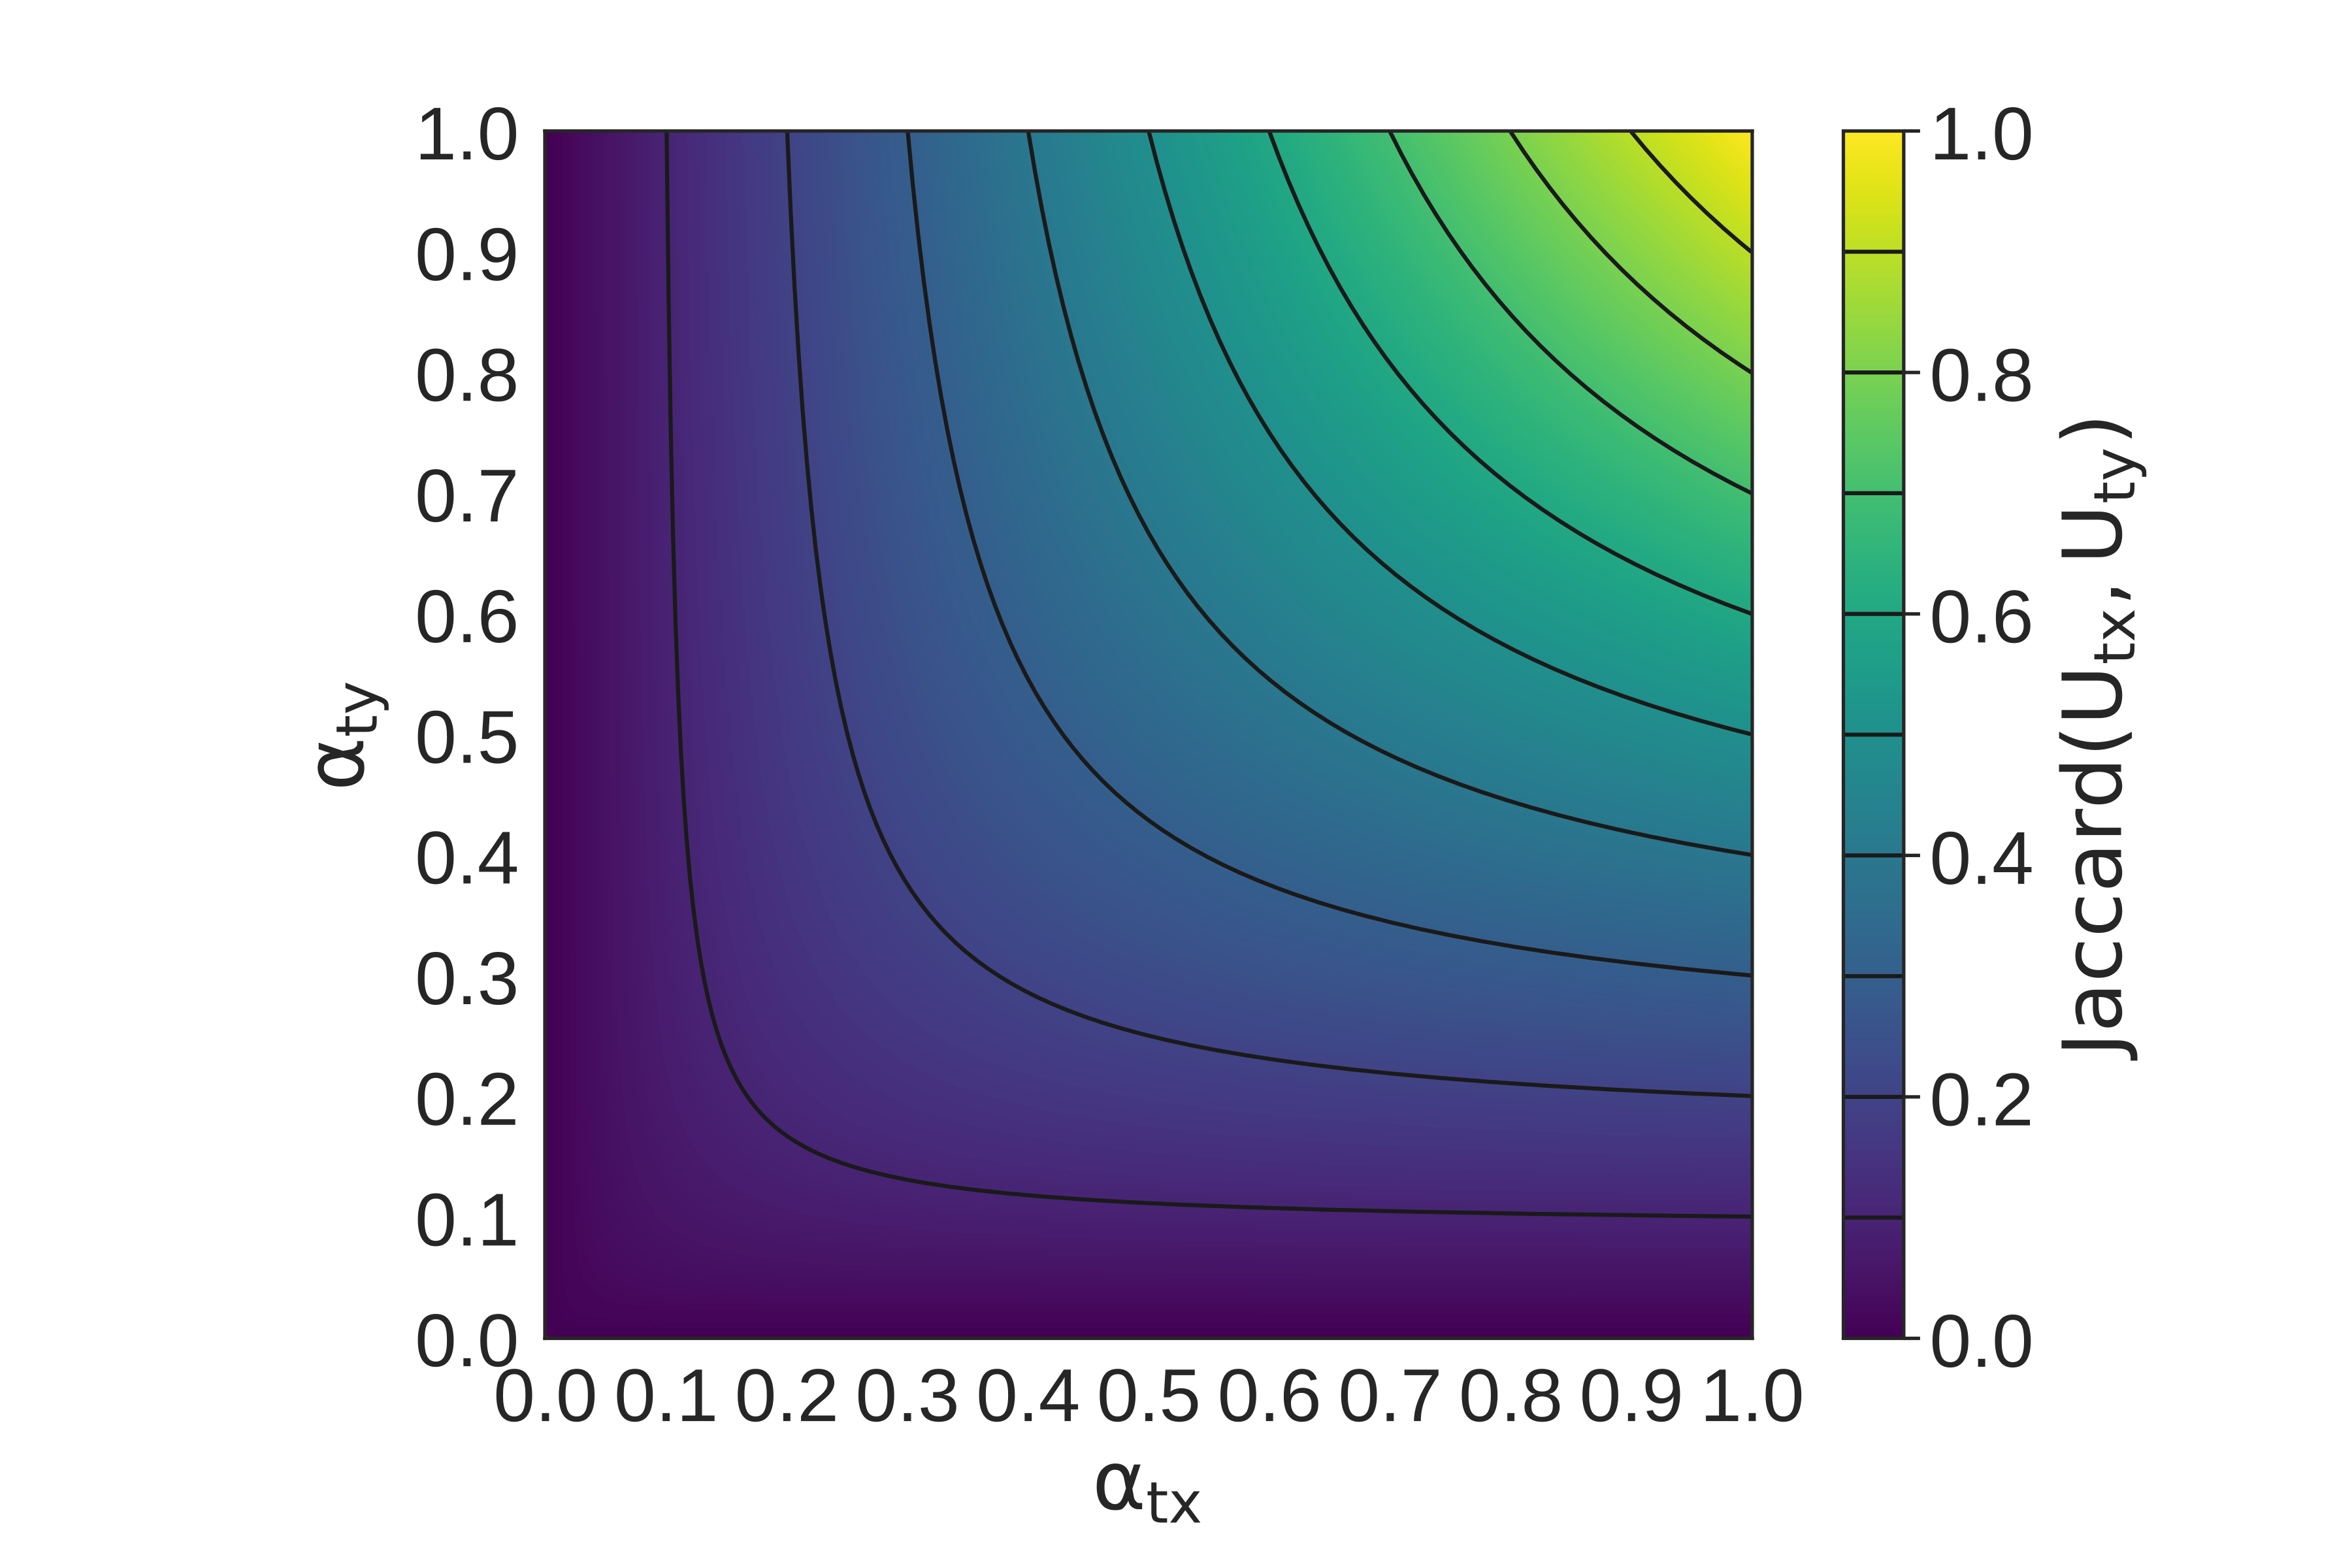
\includegraphics[width=\linewidth]{ch4.hourglass/images/math_flies.png}
    \caption{The Jaccard index landscape.}
    \label{fig:peak_math}
\end{figure}

\begin{figure}[H]
    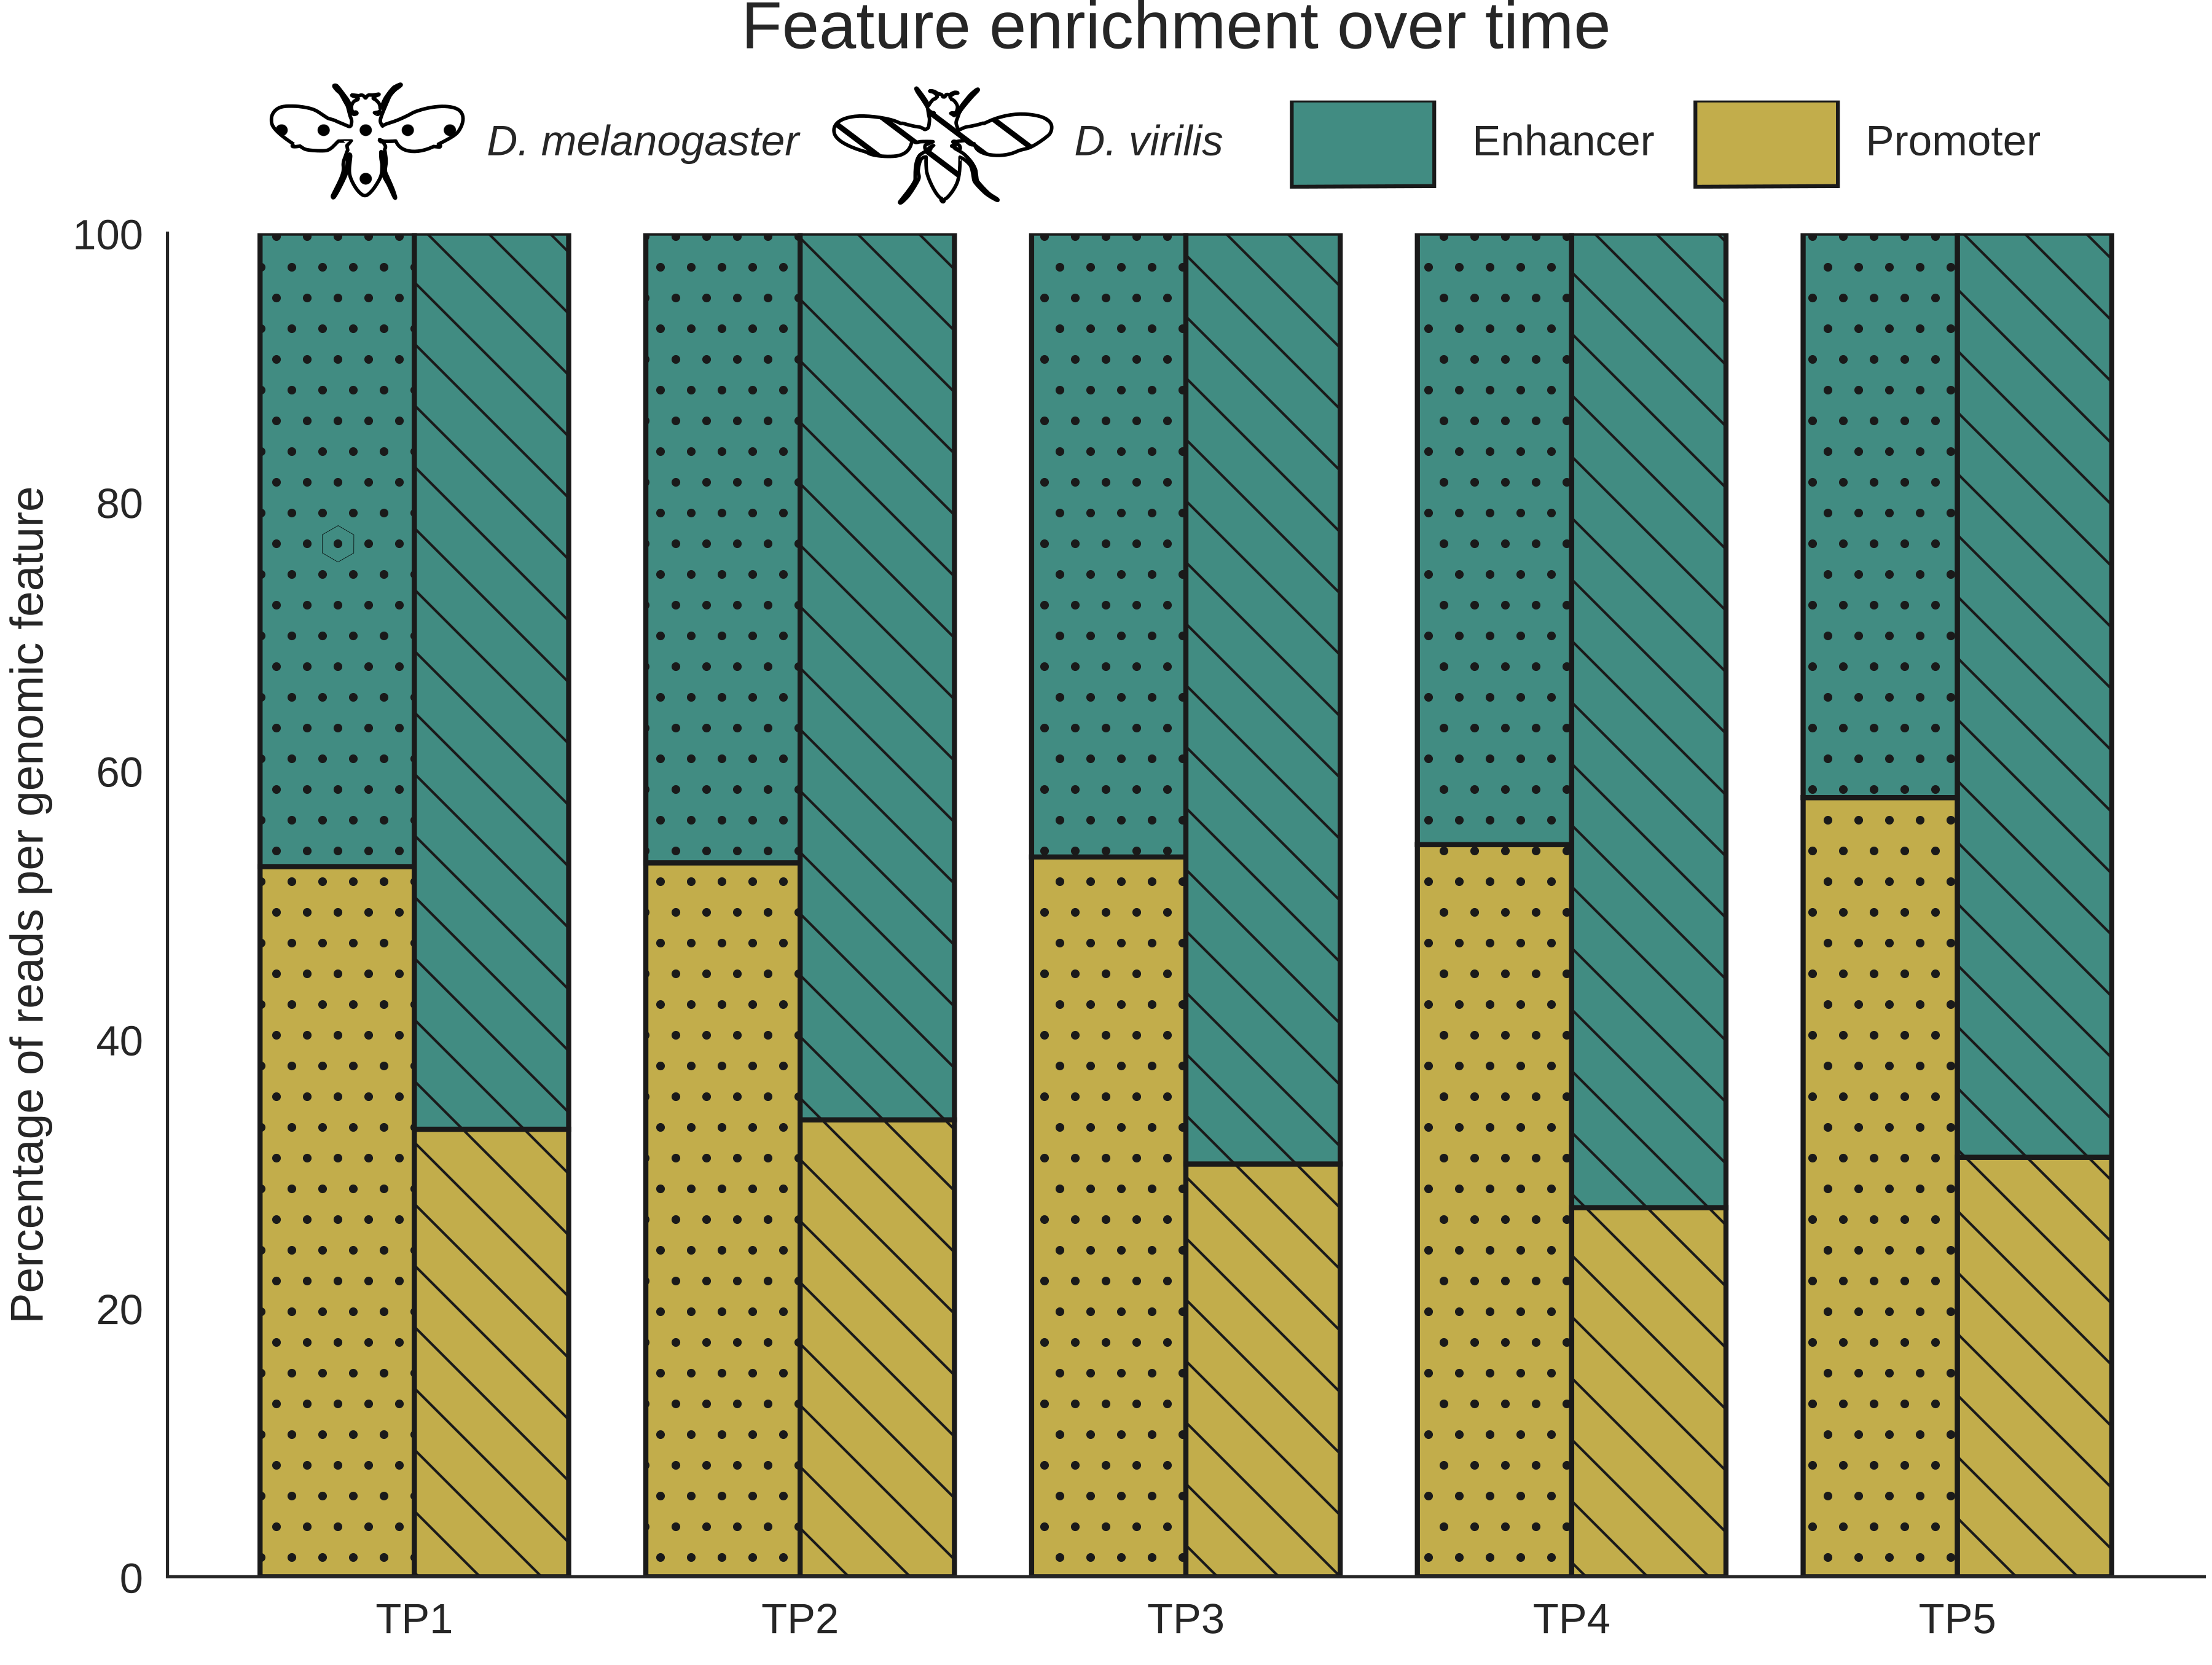
\includegraphics[width=\linewidth]{ch4.hourglass/images/feature_enrichment.png}
    \caption{explain.}
    \label{fig:peak_enrichment}
\end{figure}

\closesupplement


\chapter{Scepia}

\chapter{General discussion}
\section{The (molecular) phylotypic stage}

All models are wrong, but some are useful. 

\section{scepia: gene regulatory networks}

\section{The future of biology}

\subsection{Computational}

\subsection{lack of unified data encode like stuff}

For seq2science paper we tried paper X, Y, Z. DIFFICULT to get similar results. WHAT da fuck?

% No similarity between replicates:
% https://www.nature.com/articles/s41467-019-12687-4
% 

\subsection{Open Science}

\subsection{Too much descriptive, not enough understanding}

\subsection{Move away from mRNA}

mRNA and protein relation

https://www.biorxiv.org/content/10.1101/2023.05.23.541948v1

\subsection{Stop blaming "the incentives"}

incentives: https://www.talyarkoni.org/blog/2018/10/02/no-its-not-the-incentives-its-you/

\subsection{Self-correcting}

e.g. wild growth covid papers

papers keep on being cited after retraction

% Biology is messy, but that does not mean computational biology has to be.


\chapter{Appendix}
\section{Curriculum vitae}

TODO

\section{List of Publications}

% PubPeer comment on \textit{Genomic encoding of transcriptional burst kinetics}. \textbf{Maarten van der Sande}. https://pubpeer.com/publications/1AA141AA501FF528C34DFF944CEF8E\#1, 2023.

Genomepy: genes and genomes at your fingertips. S Frölich, \textbf{M van der Sande}, T Schäfers, SJ van Heeringen. Bioinformatics 39 (3), btad119, 2023.

Computational approaches to understand transcription regulation in development. \textbf{M van der Sande}*, S Frölich*, SJ van Heeringen. Biochemical Society Transactions 51 (1), 1-12, 2023.

Qnorm: fast-ish (and correct!) quantile normalization in Python. \textbf{Maarten van der Sande}, SJ van Heeringen
Retinoic acid signaling drives differentiation toward the absorptive lineage in colorectal cancer. RA Wester, \ldots, \textbf{Maarten van der Sande}, \ldots. Iscience 24 (12), 103444, 2021.

ANANSE: An enhancer network-based computational approach for predicting key transcription factors in cell fate determination. Q Xu, G Georgiou, S Frölich, \textbf{M van der Sande}, ..., SJ van Heeringen.Nucleic Acids Research 49 (14), 7966-7985, 2021.

Combinatorial transcription factor activities on open chromatin induce embryonic heterogeneity in vertebrates. AR Bright, \ldots, M Van der Sande, \ldots, SJ van Heeringen. The EMBO Journal 40 (9), e104913, 2021.

Stronger induction of trained immunity by mucosal BCG or MTBVAC vaccination compared to standard intradermal vaccination. MPM Vierboom, ..., \textbf{Maarten van der Sande}, ..., FAW Verreck. Cell Reports Medicine 2 (1), 100185, 2021.

A cell-based boundary model of gastrulation by unipolar ingression in the hydrozoan cnidarian Clytia hemisphaerica. \textbf{M van Der Sande}, Y Kraus, E Houliston, J Kaandorp. Developmental biology 460 (2), 176-186, 2020.

\section{references}

\renewcommand*{\bibfont}{\scriptsize}
\printbibliography[heading=none]


\end{document}
